\documentclass[a4paper,10pt]{report}
\usepackage{graphicx}
\usepackage{nomencl}
\makenomenclature
\usepackage{epsfig}
\usepackage{wrapfig}
\usepackage{amsmath}
\usepackage{psfrag}
\usepackage{a4wide}
\linespread{1.5}
\renewcommand{\nomname}{List of abbrevations and symbols}
%\pdfpagewidth 8.5in
%\pdfpageheight 11in

%\setlength\topmargin{-0.1in}
%\setlength\headheight{0in}
%\setlength\headsep{0in}
%\setlength\textheight{7.7in}
%\setlength\textwidth{6.5in}
%\setlength\oddsidemargin{0in}
%\setlength\evensidemargin{0in}
%\setlength\paragraph*indent{0.25in}
%\setlength\paragraph*skip{0.25in}

\title{\textbf{Decentralized frame synchronization of a TDMA-based wireless sensor network}}
\author{Fasika A. Assegei}
\date{August 14, 2008}
\begin{document}
\pagestyle{empty}
\begin{titlepage}
\begin{center}
\parbox{27cm}{
  \hspace{1cm}
  \begin{minipage}[c]{.6\textwidth}
    Eindhoven University of Technology\\
    Department of Electrical Engineering\\
    Telecommunications and Electromagnetism
  \end{minipage}
   \begin{minipage}[c]{.4\textwidth}
    
\includegraphics[scale=0.5]{TUElogoCompact2}
  \end{minipage}
}
\end{center}

%\begin{minipage}[c]{15cm}
%%\paragraph*pic[r]{
\epsfig{file=graphics/titlepage/TUElogoCompact2.eps,width=0.45\textwidth,clip=}}
%    Eindhoven University of Technology\\
%    Department of Electrical Engineering\\
%    Telecommunications and Electromagnetism
%\end{minipage}
\begin{center}
\hspace{2cm}
\begin{minipage}[c]{16cm}
    \vspace{2.5cm}
    \centering
    \Large
    \maketitle
    \vspace{4cm}
\end{minipage}
\end{center}
\hspace{1cm}
\begin{minipage}[b]{16cm}
    Master of Science Thesis\\
    Group: Radiocommunications (ECR)\\
    Supervisors:\\
    Frits van der Wateren ( Chess B.V.) \\
    dr.ir. P.F.M. Smulders (TU/e) \\
%    Graduation professor:\\
%    Prof.dr.ir. E.R. Fledderus
\end{minipage}
\end{titlepage}
%\thispagestyle{empty}\pagenumbering{roman}
%\setcounter{page}{-1}\cleardoublepage

%\section*{Abstract}
%Abstract goes here.
%
%\cleardoublepage
%
%\section*{Acknowledgements}
%\cleardoublepage
\pagestyle{plain}
\pagenumbering{roman}
\addcontentsline{toc}{chapter}{Abstract}
\section*{\begin{center}Abstract\end{center}}
Synchronization is a one of the main issues in the design of \textit{Wireless Sensor Networks}(WSNs). Most applications of WSNs make extensive use of synchronization mechanisms like \emph{Time Division Multiple Access} \nomenclature{TDMA}{Time Division Multiple Access} scheduling, accurate time stamping of events, coordinate activities of the network or data fusion. The unique requirements of WSNs in terms of precision, lifetime, energy and scope of the synchronization achieved, make the synchronization methods developed for centralized systems unsuitable for WSNs. This motivates the research of synchronization methods which are aligned to the specific properties of WSN.  Interfering nodes, due to mobility and newly incoming nodes, lead to instability in synchronization.  Median$\cite{median}$ algorithm is implemented currently on the wireless sensor nodes in MyriaNed$\cite{myrianed}$ project. In this research, the flaw in the Median algorithm is explored and three algorithms have been proposed to achieve a decentralized, stable, and energy-efficient synchronization of a WSN. The algorithms achieve synchronization by using the phase error of a node's wakeup time with those of the neighboring nodes, without exchanging the information about the clock time of the sender. So, the methods avoid time keeping on the messages (time stamping) which reduces the overall overload. Stability of the algorithms is simulated in a highly dynamic network. Results from simulation of the models are presented and discussed. The algorithms can be integrated with the slot allocation algorithm to form the MAC\nomenclature{MAC}{Media Access Protocol} layer protocol for a better throughput. The research is concluded with the comparison of three algorithms in terms of energy consumption and performance. A low energy-consumption or a better convergence as well as the length of the guard time can be used as a metric for selecting the algorithm.
\newpage
\addcontentsline{toc}{chapter}{Acknowledgment}
\section*{\begin{center}Acknowledgment\end{center}}
I would like to express my sincere gratitude to my supervisor, Frits van der Wateren from Chess Innovation Team, for all the support he has given me during the project. I am greatly indebted to him for all the insight and support that he showed in every phase of the project. I am grateful to dr.ir.Peter Smulders and prof.dr.ir. Peter Baltus for providing guidance during the project. \newline \newline I am greatly indebted to prof.dr.ir. Erik Fledderus for providing me the opportunity to work on such an interesting topic for my Master's thesis. He has been extremely helpful, and was always availble whenever I needed help. \newline \newline I like to express my appreciation to prof.dr.ir. Peter Baltus and prof.dr.ir. Jean-Paul Linnartz for taking time to serve on my thesis panel.\newline \newline  I want to say thanks for everyone in Chess Innovation team (Pieter, Wouter, Bert, Roland) for the wonderful time that I had working at Chess. They are exremely helpful and make the environment lively. It has been a pleasure working with them. \newline \newline Special thanks to my friends, Simon and Aman, and the all-in gang in Eindhvoen (Yenu, Teme, Esae and Frew). I want to thank all my friends at TU/e, for their help and encouragement and for making my stay in the Netherlands unforgettable.\newline \newline  Finally, I want to extend my gratitude to my family. No words can describe how grateful I am to my mohter, Etye and my sister, Hanna, and my brother, Teddy who showed immense faith in me. Thanks.
\newpage
\addcontentsline{toc}{chapter}{Contents}
\tableofcontents
\addcontentsline{toc}{chapter}{List of figures}
\listoffigures
\addcontentsline{toc}{chapter}{List of Abbrevations and symbols}
\printnomenclature[3.5cm]
\chapter{\textbf{Introduction}}
\pagenumbering{arabic}
\section{\textbf{Wireless sensor networks}}\par
Technological advances have led to the development of low-cost sensors, which are capable of wireless communication and
data processing. WSNs\nomenclature{WSN}{Wireless Sensor Network} are distributed networks of such sensors, dedicated to closely observing real-world phenomena. Such sensors can be embedded in the environment or enabled with mobility. They can be deployed in
inaccessible, dangerous or hostile environments. The sensors need to configure themselves in a communication network in order to collect information that has to be pieced together to have a broader picture of the environment than what each sensor individually
senses. Various applications are realized using sensor networks$\cite{10}$. As the WSNs become an integral part of the modern era, addressing issues in designing such networks becomes necessary.
\paragraph*{} One of the design issues in WSN technology is synchronization, which is a critical piece of infrastructure in any
distributed system. In sensor networks, a number of factors makes flexible and robust time synchronization particularly important and
more difficult to achieve than in centralized networks. Collaboration among nodes is often required for different purposes$\cite{11}$. A common view of physical time is a basic requirement for nodes to reason about events that occur in the physical world. In addition to these domain-specific requirements, sensor network applications often rely on synchronization as typical distributed systems do. These applications include proper \textit{Time Division Multiple Access} (TDMA) scheduling, coordination of future action and interaction with users$\cite{1}$.
\section{\textbf{Existing work on WSN synchronization}}\par
Several algorithms have been proposed and researched for synchronization in WSNs. The \textit{Reference Broadcast
Synchronization} (RBS)\nomenclature{RBS}{Reference Broadcast
Synchronization} stated in $\cite{2}$ is an important scheme in the
area of WSN synchronization. It achieves a Receiver-Receiver
pairwise synchronization to remove sender nondeterminism and results
in a precision of a few microseconds. It also provides clock
frequency estimates between two receivers using a linear regression
technique. But a central node is needed for broadcasting reference
signals in order to achieve synchronization. Another method for
achieving a network-wide synchronization is suggested by
$\cite{texas}$. This approach establishes a time conversion table
between clocks of two nodes using different estimation techniques.
This method has a higher overload as it involves the transfer of
sender's clock time and a central node is needed for the
synchronization.
\paragraph*{}
Another approach to a decentralized slot synchronization for
TDMA-based networks is presented in $\cite{3}$. It uses the topology
of the nodes as a means to weigh the phase error of the sender with
the receiver.In this case, higher message overhead is observed in
sending the degree of connection (topology information) as a method
of synchronization. A different approach to weight-based
synchronization for interference elimination for a TDMA based ad-hoc
networks is presented in $\cite{6}$. The algorithm achieves
synchronization in a decentralized manner using the nodes offset
with its neighbors with a goal of eliminating the interference. The
algorithm achieves synchronization by eliminating the impact of
interference nodes. But this method directly eliminates nodes which
are newly joining or interfering nodes. Correlation method is used
in $\cite{correlation}$ in order to decode the message and learn
about the status of the sender node which is used for
synchronization. High message overhead is the setback of the
algorithm. A decentralized method is introduced in $\cite{median}$
which uses the average of the phase errors to adjust the wakeup time
of the node. Even though this method is simple, the method is highly
vulnerable in dynamic networks.
\section{\textbf{Objective and overview of the research}}
Upon the literature survey performed, it is observed that some of
the synchronization schemes use a central (master) node in order to
achieve a synchronization with the nodes. Upon the methods which
uses the decentralized methods, interference and mobility are the
least addressed issues. Since nodes are subjected to severe changes
in environmental conditions, the accuracy of these synchronization
schemes might suffer a lot due to the dynamics of the network. As
part of the MyriaNed project, Median is used in the synchronization
of the wireless sensor nodes implemented in the project.
\paragraph*{}
The primary objective of this research is to address the problems in the Median and develop an algorithm to achieve a decentralized and stable synchronization of a WSN in an energy-efficient method. The algorithm is aimed to replace the currently implemented Median algorithm.  Hence, three algorithms are proposed and compared with Median algorithm in terms of performance and energy consumption. The methods use the phase errors between the receiver and its neighbors, without estimating the neighbor's clock as a way of achieving long-term synchronization. Through integration with the MAC layer protocol, a better throughput can be obtained. The algorithms developed have the following characteristics: provides higher precision, adaptive to environmental effects, energy-efficient and achieve long-term synchronization.
\paragraph*{} The remainder of the report is organized as follows:  Chapter 2 presents a general overview of synchronization in WSN and the need for a synchronized time. Chapter 3 discusses the synchronization error and discusses the problem associated with the Median algorithm. Chapter 4 presents the mathematical models of the proposed algorithms for the synchronization of the network. In Chapter 5, simulation results are presented. Analysis of the results in addition to the comparison of the methods with respect to energy consumption are discussed. Finally, Chapter 6 draws the conclusions from the research and suggests future work.
\chapter{\textbf{Synchronization in wireless sensor networks}}
\section{\textbf{Introduction}}
Chess$\cite{chess}$ created a MAC protocol for gossip communication, gMAC, for the wireless sensor network project, MyriaNed, with the gossiping technique in mind. Being a wireless sensor network, the duty cycle of the network is small, around 1$\%$. Looking back at the 1$\%$ active time versus the $99\%$ nonactive time ratio, it is a non-trivial matter to keep the network synchronized.
\paragraph*{}
A number of approaches have been introduced for different multiple access techniques, of which CSMA \nomenclature{CSMA}{Carrier Sense Multiple Access} and TDMA are the most common. One problem with CSMA is the time that passes when the radio is busy with idle listening time. Nodes need to listen to the radio for periods of time before they can actually send data.
\paragraph*{}
In TDMA, time is divided into discrete slots. Nodes transmit in rapid succession in one slot and listen in the others. In theory, there will not be any idle listening. There are some pitfalls to this approach. Firstly, the clocks of the nodes are less than perfect; they will never run at exactly the same clock-speed. To keep the nodes synchronized and
thus to let them share the same schedule, the small timing error needs to be compensated. Second, there has to be a certain algorithm
to allocate the slots among the nodes. They cannot simply all start broadcasting in the first slot, since that would cause nothing but
collisions. The research on slot allocation algorithms is being conducted alongside this research$\cite{pieter}$.
\section{\textbf{Synchronization in centralized networks}}
In a centralized system, the solution to clock drift is trivial. The centralized server will dictate the system time because time is unambiguous. With the centralized concept in mind, different protocols have been proposed and implemented to achieve synchronization in those networks, \textit{Network Time Protocol} (NTP)\nomenclature{NTP}{Network Time Protocol} being the most popular$\cite{5}$.
\paragraph*{}
Due to the infrastructure advantage, NTP is one of the most accurate
and flexible means of sending time over the Internet. The protocol
is designed to compensate for some, but not all, network time delays
between the server and the client. NTP is most successful across
local area networks and can give accuracy as good as a few
milliseconds. On the world wide web, however, time transfer delays
are at the mercy of server traffic and network bottlenecks, and
accuracy figures cannot be quoted as easily. NTP uses a round time
delay to a universal time reference so that it can adjust the clock
of the networked component. It measures delays within the network
and within the algorithms on the machine on which it is running.
Using  these tools and techniques, it is able to synchronize clocks
to within milliseconds of each other when connected on a Local Area
Network and within hundreds of milliseconds of each other when
connected to a \textit{Wide Area Network}
(WAN)\nomenclature{WAN}{Wide Area Network}. Figure $\ref{ntp}$ shows
the simplified structure of how the NTP protocol works to
synchronize client computers.
\begin{figure}
\centering
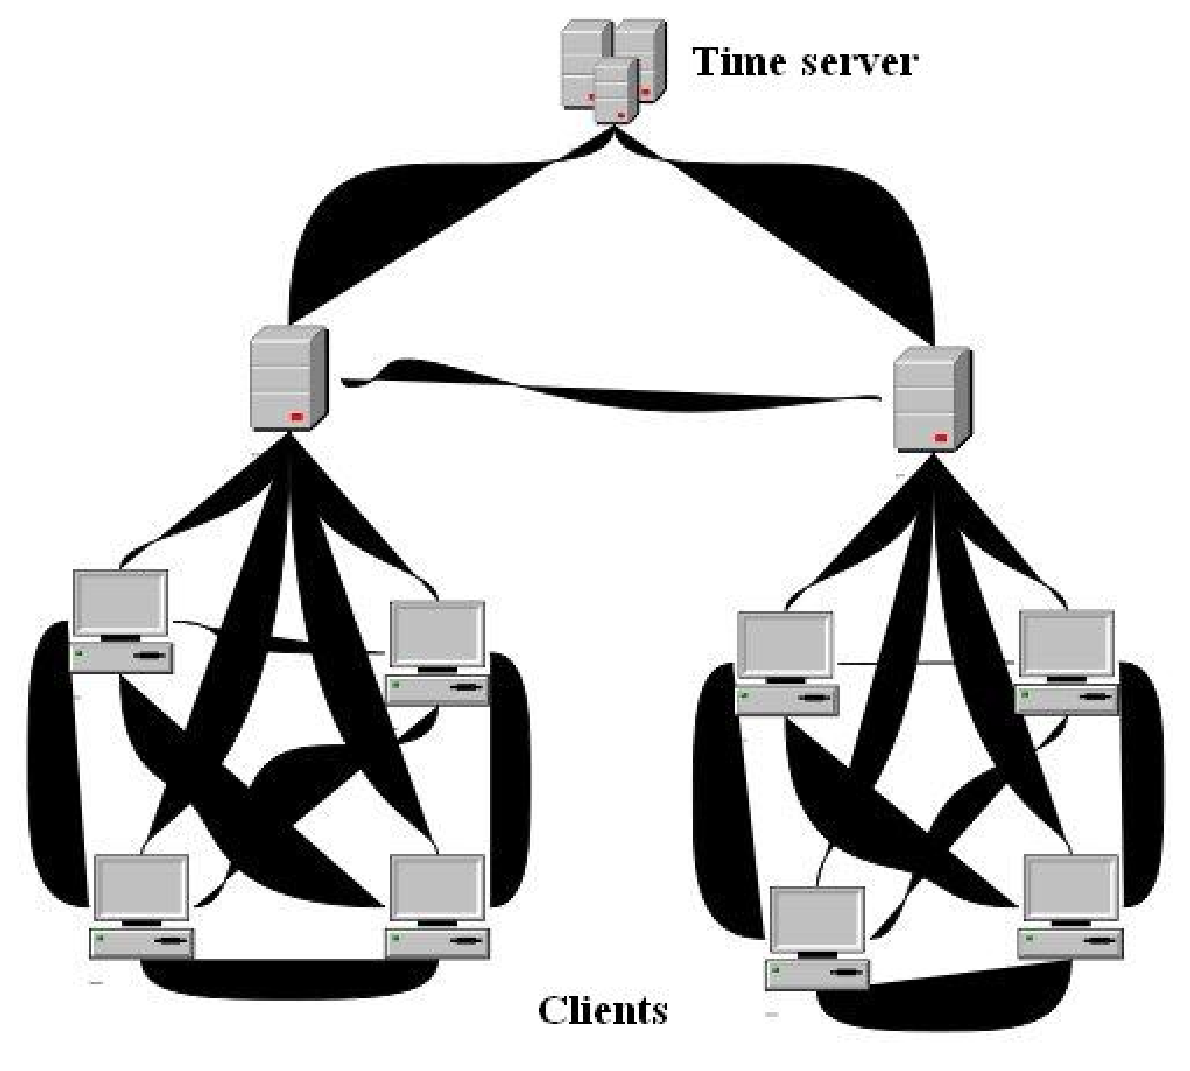
\includegraphics[width= 0.5 \textwidth]{ntp}
\caption{A simple NTP diagram} \label{ntp}
\end{figure}
The tiered nature of the NTP time distribution tree enables a user to choose the accuracy needed by selecting a level (stratum) within
the tree for machine placement. A time server placed higher in the tree (lower stratum number), provides a higher likelihood of
agreement with the \textit{UTC}\nomenclature{UTC}{Coordinated Universal Time} standard.
\paragraph*{}
Synchronization in distributed systems takes a different kind of
approach since there is no central authority to be referred in case
of time requests. Central nodes can be assigned as to play the role
of a server as in the case of the centralized system. But, most of
the time, distributed systems, due to their unique properties, have
no central command. Development of a synchronization scheme that
satisfies such requirements is challenging. The task becomes
particularly daunting in WSNs, in light of their additional domain
requirements. Before exploring the specific requirements of WSN, a
discussion about the need of a synchronized time is presented.
\section{\textbf{The need for a synchronized time}}
There are many reasons why a synchronized time is needed in a WSN. Some of them include data integration, TDMA scheduling, target
tracking and localization. Two of the most common areas where synchronization is a necessity are described below.
\subsubsection{Data Integration}
Data collection is the main task of the sensor nodes, hence data gathering and integration is a crucial component. The signal processing literature sometimes refers to this as array processing; with heterogeneous sensors, it is often called \textit{data fusion}.
\begin{figure}
\centering
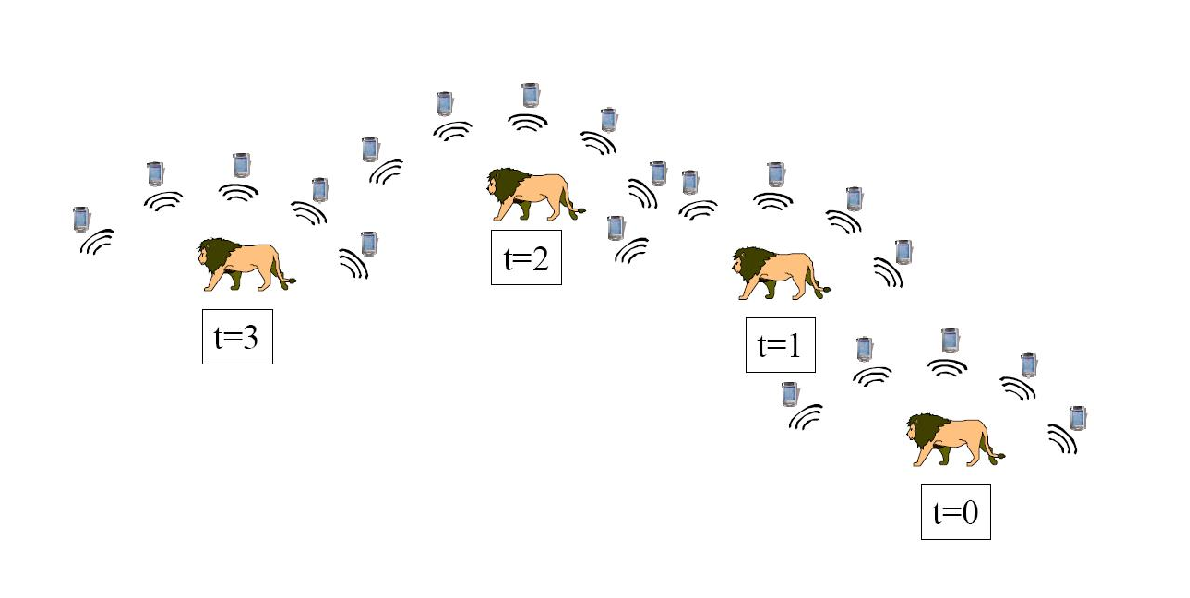
\includegraphics[width= 0.6\textwidth]{lions}
\caption{Tracking the movement of an object}
\label{lions}
\end{figure}
There are many applications which need data fusion such as signal enhancement (noise reduction) and source localization. It would seem to be a natural match to implement such algorithms in distributed sensor networks, and there has been great interest in doing so. However, much of the extensive prior art in the field assumes centralized sensor fusion. That is, even if the sensors gathering data are distributed, they are often assumed to be wired into a single processor. Centralized processing makes use of implicit time synchronization. Sensor channels sampled by the same processor also share a common time base. Figure $\ref{lions}$ shows one example of data fusion application. In order to locate the moving object, in this case the lion, nodes have to have a common notion of time. Upon integration, not only the location of the lion but also the time when the lion was spotted is necessary. So, having the same notion of time is important.
\subsubsection{TDMA slot alignment}
As it is implemented in WSN, the duty cycle is of prime importance due to the energy requirement of the nodes. A duty cycle is the fraction of time that a system is in an "active" state. Major benefits can be achieved by using this scheduled communication/sleeping protocol:
\begin{itemize}
\item Low duty cycles - a node can operate in low duty cycles, hence reducing the energy consumption of the nodes.
\item Efficiency in transmission - a sender can efficiently transmit a message to its neighbors by just waking up and sending exactly when a receiver is listening.
\item Efficiency in receiving - a receiver can schedule its own time intervals to receive a particular neighboring transmitter.
\end{itemize}
\begin{figure}
\centering
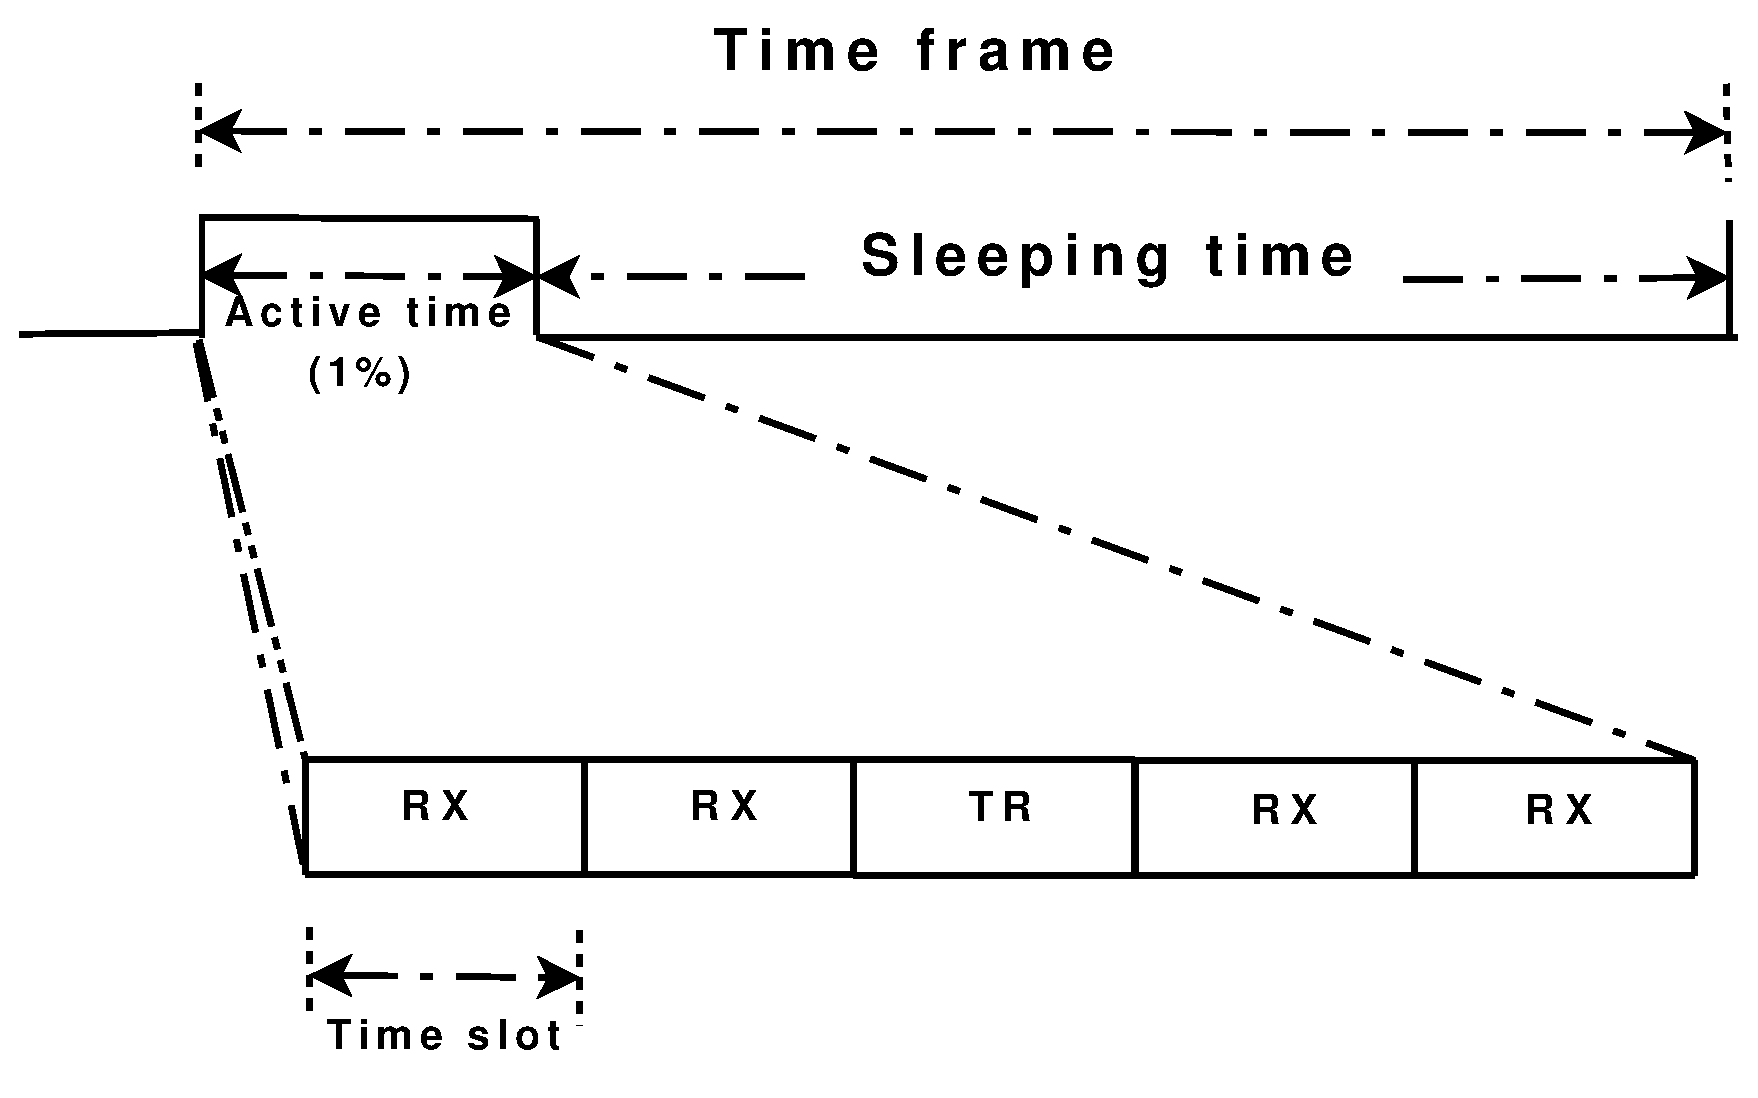
\includegraphics[width=0.5 \textwidth]{tdmaframe}
\caption{TDMA frame} \label{tdmaframe}
\end{figure}
The scheduled communication/sleeping protocol, the multihop scheme and the rippling of the message through the network are best implemented using a TDMA scheme. Usually, this medium access scheme is best suited for the infrastructure mode where the base stations schedule the TDMA slots for each node. However, such structure is not used in WSN. The scheduling of the TDMA slots is made locally by reaching an agreement between direct neighbors. As previously stated, the WSN being developed at Chess uses a TDMA protocol for channel access, hence the reason for synchronization. TDMA is a channel access method for shared medium networks. It allows several users to share the same frequency
channel by dividing the signal into different time slots. The users transmit in rapid succession, one after the other, each using its
own time slot. This allows multiple stations to share the same transmission medium while using only the part of the bandwidth they
require. Figure $\ref{tdmaframe}$ shows how a time frame is divided into receiving and transmitting slots. In the time frame, the active slot is divided into one transmitting slot and many receiving slots.
\paragraph*{}
In this approach, nodes use time slots in order to communicate with each other. It is considered that two nodes have
their TDMA schedule synchronized when the numbers of the current time slot of any of the TDMA schedules involved are the same for any
given moment in time. The types of the slot may be different, TX or RX. To successfully initiate a network, the nodes has to be
synchronized and capable to send and receive messages. To establish a link between neighboring nodes, a particular node needs to know
the schedule of all its neighbors, which is the purpose of the slot allocation algorithm. The MAC protocol used in MyriaNed is the gMAC$\cite{pieter}$. The g in gMAC comes from Gossiping, which represents the gossip protocol implemented in the network layer$\cite{gossip}$.
\paragraph*{}
Each neighbor has a different transmitting slot so that there will
be no collision. As shown in Figure $\ref{tdmasch}$, the
transmission slots of the nodes are at different times. Thus, a
message transmitted should be received in the receiving slot of the
neighboring nodes. In order to have a seamless communication between
the nodes, the synchronization of the frames is a necessary part.
The processing element and other functions on a WSN operate on a
local clock. Due to physical factors, the frequency of the
oscillator has drift. When no provisions are taken, it causes the
nodes to run out of sync. Given that there is a certain error, the
node has to adjust it's wakeup time at the end of the last receiver
slot in order to synchronize with the neighbors.
\begin{figure}
\centering
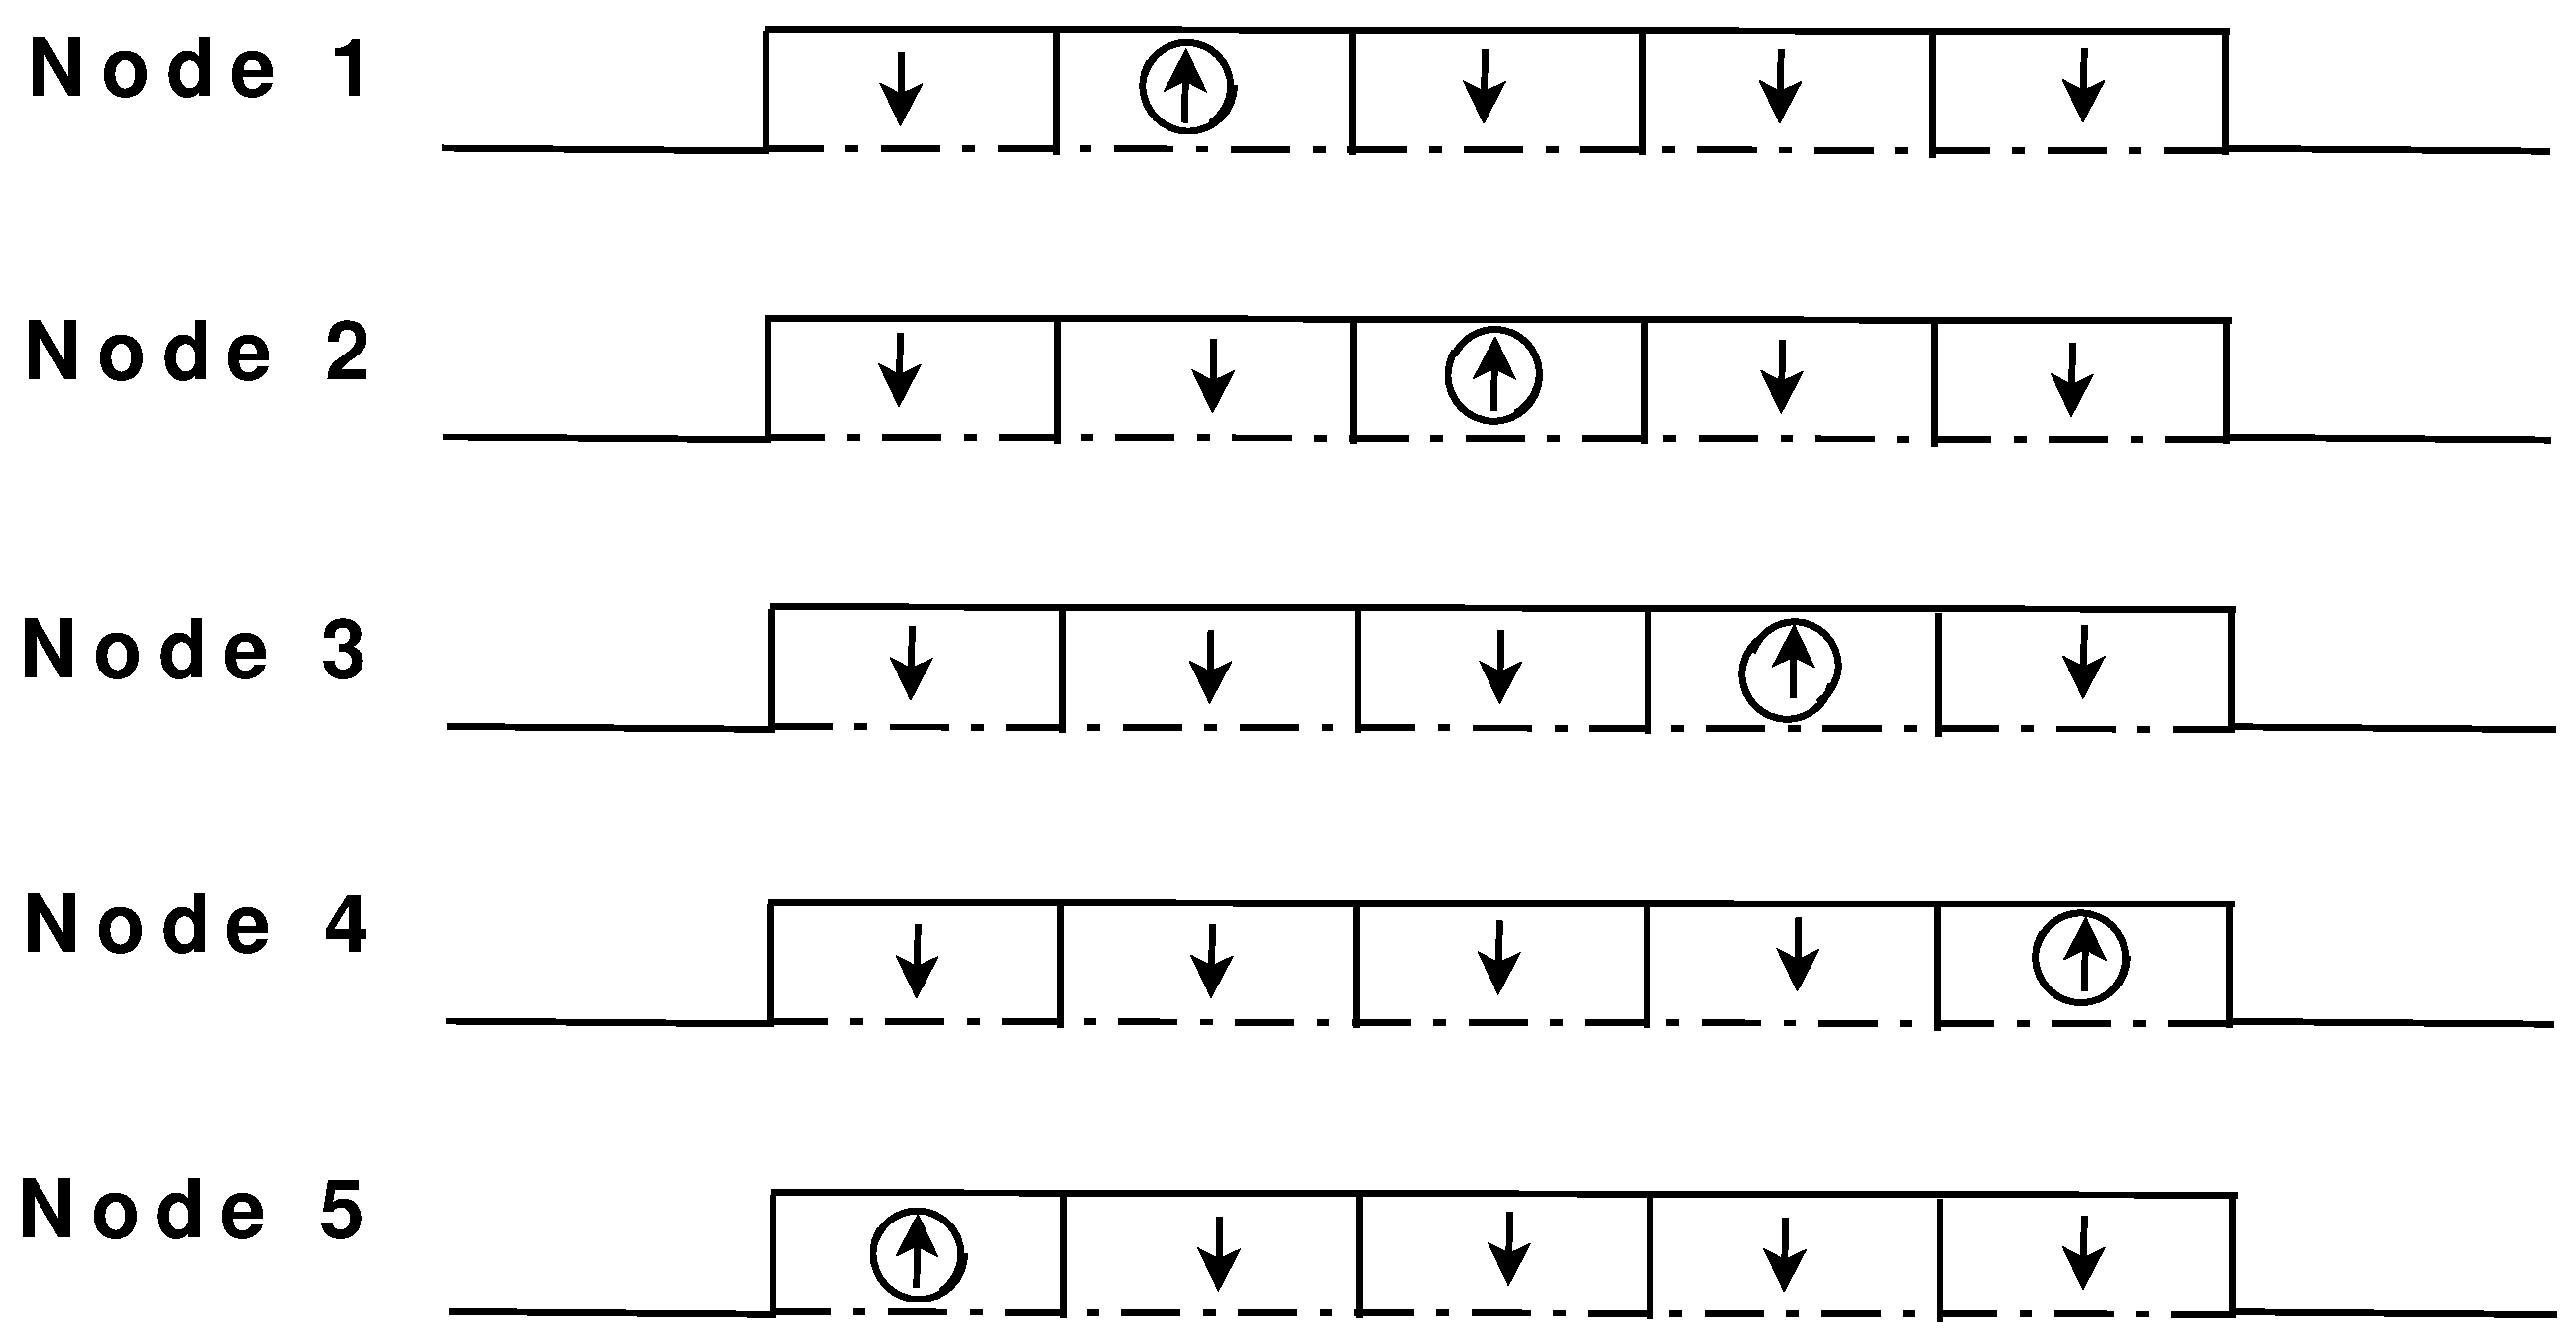
\includegraphics[width=0.5\textwidth]{tdmaschedule}
\caption{TDMA channel access} \label{tdmasch}
\end{figure}
\paragraph*{}
The drift in the node's clock causes the TDMA slot boundaries to drift when we compare two nodes with the same schedule. Hence, the need for synchronization is vital for the seamless communication of the nodes. But synchronization in WSNs is more challenging, which is explained in the next section.
\section{\textbf{Wireless sensor networks: Why different ?}}
Are synchronization methods developed for centralized systems applicable in the case of WSNs? Many assumptions in the centralized schemes do not hold in the case of WSNs. Some of these factors can be described as follows:
\begin{itemize}
\item \textbf{Energy limitation}: Due to their small size and nature of applications which they are designed for, energy consumption is a major concern in a WSN. Nodes are mostly battery-powered and are expected to run for a long time before they run out of power. An energy efficient method is a requirement for WSNs synchronization.
\item \textbf{Dynamic nature of the network}: In a centralized system, the topology remains more or less static even if there are physical
dynamics involved  in some centralized systems like \textit{GSM} \nomenclature{GSM}{Global System for Mobile communications}. In a WSN, network dynamics results from various factors like mobility of nodes, node failures and environmental obstructions, which prevents simple static configurations. Hierarchical structures might get nodes poorly synchronized, and nodes might not be connected when they need
synchronization the most.
\item \textbf{Diverse applications}: WSNs are used for a variety of applications, which can have totally different needs as far as synchronization is concerned. For example, localization applications need a short-lived but highly
precise synchronization, while target tracking applications can tolerate a little lower precision, but want the synchronization to
last longer. Some applications might need a global timescale while some others can work with a local timescale.
\item \textbf{Cost of the nodes}: Sensor nodes are very small in size and must be cheap cost wise since they are implemented in large
numbers. Now, a very good synchronization with \textit{GPS}\nomenclature{GPS}{Global Positioning System} receivers can be obtained, but it will be unreasonable to put an expensive and energy-hungry GPS receivers on a sensor node.
\end{itemize}
All of the factors mentioned above make the problem of time synchronization more challenging in case of WSNs. Keeping this in mind, we can formulate some design requirements for WSN frame synchronization.
\section{\textbf{Requirements of the algorithm for MyriaNed}}
\subsubsection{\textbf{Precise synchronization}}
Synchronization cab be of two types: Course and Precise synchronization. Course synchronization is implemented when a node is joining in the network. After a newly joining node listened the synchronization information sent by the other nodes in the network, it adjusts its time slot reference to the time when it detects the synchronization information, which includes the propagation delay. Precise synchronization is implemented when a node has already joined the network, which repeatedly adjusts the diversion of its time slot reference caused by propagation delay and clock drift. In this research, we focus on precise synchronization.
\subsubsection{\textbf{Lifetime}} Lifetime is the interval that clocks remain synchronized, or the interval over which a particular
timescale is defined. Sensor networks need synchronization over a wide range of lifetimes, ranging from less than a second to a longer period. In our implementation, the length of lifetime required for synchronization is throughout the life time of the network since
the primary reason for the synchronization of the MyriaNed network is for TDMA frame synchronization.
\subsubsection{\textbf{Scope}} The scope is the size of the region in which a timescale is defined. In some cases, the scope may be purely geographic (e.g., distance in meters). In other contexts, it is more useful to think about the logical distance, such as the number of hops through a network. Naturally, these two forms are correlated in a sensor network, scaled by its radio's nominal range. A node moving across the field, should be synchronized to the remaining nodes, which it might join again after some periods. A disruption of communication can also result in the disappearance of a node where after some periods of out-of-sight,
a communication link can be established again. During the
'come-back', the node should be able to adapt its clock to the
remaining nodes in the neighborhood.
\subsubsection{\textbf{Internal vs. External Synchronization}}
In many distributed systems, synchronization simply means adjusting the clock to a correct time from an outside source. This
definition implies that a notion of the correct time, such as UTC, exists. However, in sensor networks, UTC is not always needed. There are situations where distributed nodes need to be synchronized, but not necessarily with the absolute time.
In many cases, the exact time at which the action is executed is far less important than ensuring that all nodes act simultaneously. This includes TDMA frame alignment. This function requires internal or relative synchronization: the network must be internally consistent, but its relationship to outside time standards is not needed or known.
\subsubsection{\textbf{Energy budget}} The need for energy efficiency permeates virtually in all aspects of sensor networks design. The exact energy constraints are difficult to quantify because there is a wide range of hardware found across the spectrum of network
implementations, and often within a single network. Some nodes have high power batteries and run all the time; others are so constrained that they only wake up occasionally, take a single sensor reading, transmit it and then immediately returning to sleep.
%\subsubsection{\textbf{Convergence Time}} The importance of convergence time as a metric is directly tied to the need for energy efficiency. If energy would not be a concern, the chosen form of synchronization could simply be left running continuously. Though convergence time might be important due to its effect on network start-up, it would make no difference in the steady-state. However, in this energy-constrained world, systems are often forced to power down as many services as possible for as long as possible. This makes convergence time important to consider.
\subsubsection{\textbf{Simplicity}} Extra overhead in the adds up to more computational cost. This in turn has a disadvantage in the energy-constraint WSN. A simple message is preferable although it passes most of the burden to the synchronization algorithm to determine the next wakeup time of the node.
%\paragraph*{}These complications are startling to look for a new arena for the synchronization of WSNs.
\chapter{\textbf{Problem formulation}}
\section{\textbf{Sources of synchronization error}}
The first step in designing any time-synchronization algorithm would be to understand why and where it is required. The different factors which give rise to errors between the clocks of two nodes can be divided into two main categories$\cite{texas}$:
\begin{enumerate}
\item \textbf{Oscillator Characteristics}: The sensor nodes' clocks run on very cheap oscillators. The following two properties are prone to error.
         \begin{description}
         \item \emph{\textbf{Accuracy}}: This is a measure of difference between oscillator's expected (ideal) frequency and actual frequency.
         \item \emph{\textbf{Stability}}: This is the oscillator's tendency to stay at the same frequency over time. There can be short-term instability due to environmental effects, supply voltage, long-term instability due to temperature effects and crystal aging.
      \end{description}
\item \textbf{Hardware and environmental factors}: The non-determinism in the message delivery latency is a major source of error in any synchronization algorithm, when applied into real sensor networks. This can be categorized in four type of delays:
      \begin{description}
         \item \emph{\textbf{Send time}}: The time spent at the sender to build the message, i.e. the time duration between generating the message and injecting it into the network.
         \item \emph{\textbf{Access time}}: Delay occurred while waiting for access to the transmit channel.
         \item \emph{\textbf{Propagation time}}: Time required for the message to travel from sender to receiver.
         \item \emph{\textbf{Receive time}}: Time needed for processing at the receiver's network interface.
      \end{description}
\end{enumerate}
Even if two clocks are assumed to have the same frequency and no drift, the above mentioned delays in the network result in phase
error between two clocks. This is because when the message from the sender reaches a receiver, the receiver adjusts its clock according to the received message. But the sender's clock changes in the mean time due to network delays. For a network of nodes, delays give rise to errors in accuracy from an ideal clocks. \paragraph*{} \noindent
     Below are presented definitions which are used throughout the report.
\begin{description}
\item \textbf{Phase error}: The oscillators of any two nodes can be out of phase at any given time, resulting in different time on both clocks. There can be some initial difference between nodes' clocks at the start of a synchronization procedure. It describes how far apart are the clocks at a given time.
\item \textbf{Frequency error}: Frequency error measures the difference in the clock rates. This metric is important because it predicts the growth of phase error over time. That is, if clocks are perfectly synchronized now, at what rate are they drifting apart? How well will they be synchronized in 60 seconds?
\item \textbf{Clock drift}: It is not just that the clocks are running at different rates, but even the frequency of each clock does not stay constant over a period of time. Clock drift arises from the instability of oscillators. For instance, if each clock drifts at a rate of $\theta$ msec/sec, then maximum relative drift between two clocks can be 2$\theta$ msec/sec.
\item \textbf{Wakeup time}: Wakeup time \nomenclature{\textit{wakeup time}}{Time that the node starts listening.} is the time that the node starts to listen to the channel.
\item \textbf{Clock cycle (\textit{clk})}: A clock cycle \nomenclature{\textit{clk}}{A clock cycle} is the time between two adjacent pulses of the oscillator. The number of these pulses per second is the clock speed, measured in kHz, MHz.
\end{description}
\section{\textbf{Clock and frequency standards}}\par
The quality of a clock usually amounts to its frequency stability which is the ability of its frequency standard to emit
events at a constant frequency over time. The absolute value of the frequency compared to the desired value or, its frequency accuracy
is also important. Calibration can easily compensate for an inaccurate but stable clock.
\paragraph*{} As per our motive to a synchronized clock, clocks are very important in this research. The error bound achieved by a clock synchronization method is linked to both the error inherent in the method itself, and the stability of the clock's frequency. In fact, to some extent, the two are interchangeable. Stable clocks can compensate for a synchronization channel between them that is prone to large but unbiased errors. Many synchronization events can be averaged over a long time. Similarly, a precise synchronization
channel can compensate for a poor-stability crystal oscillator whereas frequent synchronization minimizes the time in-between when the
clock is left to fend for itself.
\paragraph*{}
Many types of frequency standards exist. In general, as the stability and accuracy of the clocks increase, so do their power requirements, size, and cost, all of which are important in WSNs. Most commonly found in computer clocks are quartz crystal oscillators, characterized by $\cite{6}$. Quartz crystals are attractive because they are inexpensive, small, use little power, and perform surprisingly well despite their low resource requirements. The frequency generated by a quartz oscillator is affected by a number of environmental factors: the voltage applied, the ambient temperature, acceleration in space (e.g., shock or altitude
changes), magnetic fields, and so forth. More subtle effects as the oscillator ages also cause longer-term frequency changes. The
inexpensive oscillators commonly found in computers have a nominal frequency accuracy on the order of between $10^4$ to $10^6$ that is, two similar but uncalibrated oscillators will drift apart between 1 and 100 microseconds every second, or, between about 0.1 and 10 seconds per day $\cite{6},\cite{7}$. However, their frequency stability is significantly better with a change in frequency of one
part in $10^9$ to $10^{11}$ when averaged over several seconds or more. In our implementation, a 32 kHz crystal clock $\cite{18},\cite{19}$  is used in the MyriaNode$\footnote{MyriaNode is the sensor node which is built for the project MyriaNed.}$.
\subsection{\textbf{Clock time}}
In this section, we will see the clock time and its expression. From the definition of frequency:
\begin{equation}
f = d\phi/dt \label{freq_defn} ,
\end{equation}
and integrating both sides over time,
 \begin{equation}
\phi =\int f(t)dt ,
 \end{equation}
where $f$ is frequency, $\phi$ is phase, and $t$ is time.\paragraph*{} \noindent
Thus, the clock time is described as
\begin{equation}
C(t) = \dfrac{1}{f_o}\int_{t_o}^{t} {f(\tau)d\tau} + C(t_o) ,
\label{clock}
\end{equation}
where $f(\tau)$ is the frequency of the clock, $f_o$ is the nominal frequency of the crystal oscillator and $t_o$ is the start time of
the node. The exact clock drift is hard to predict because it depends on environmental influences (such as temperature, pressure
and power). One can usually assume that the clock drift of a crystal clock doesn't exceed a maximum value $\rho$ where $\rho$\nomenclature{$\rho$}{Maximum clock drift} represents the maximum clock drift. Figure $\ref{clocktime}$ shows the relationship between clock time and absolute time for different drift rate $\rho$.
\begin{figure}
\centering
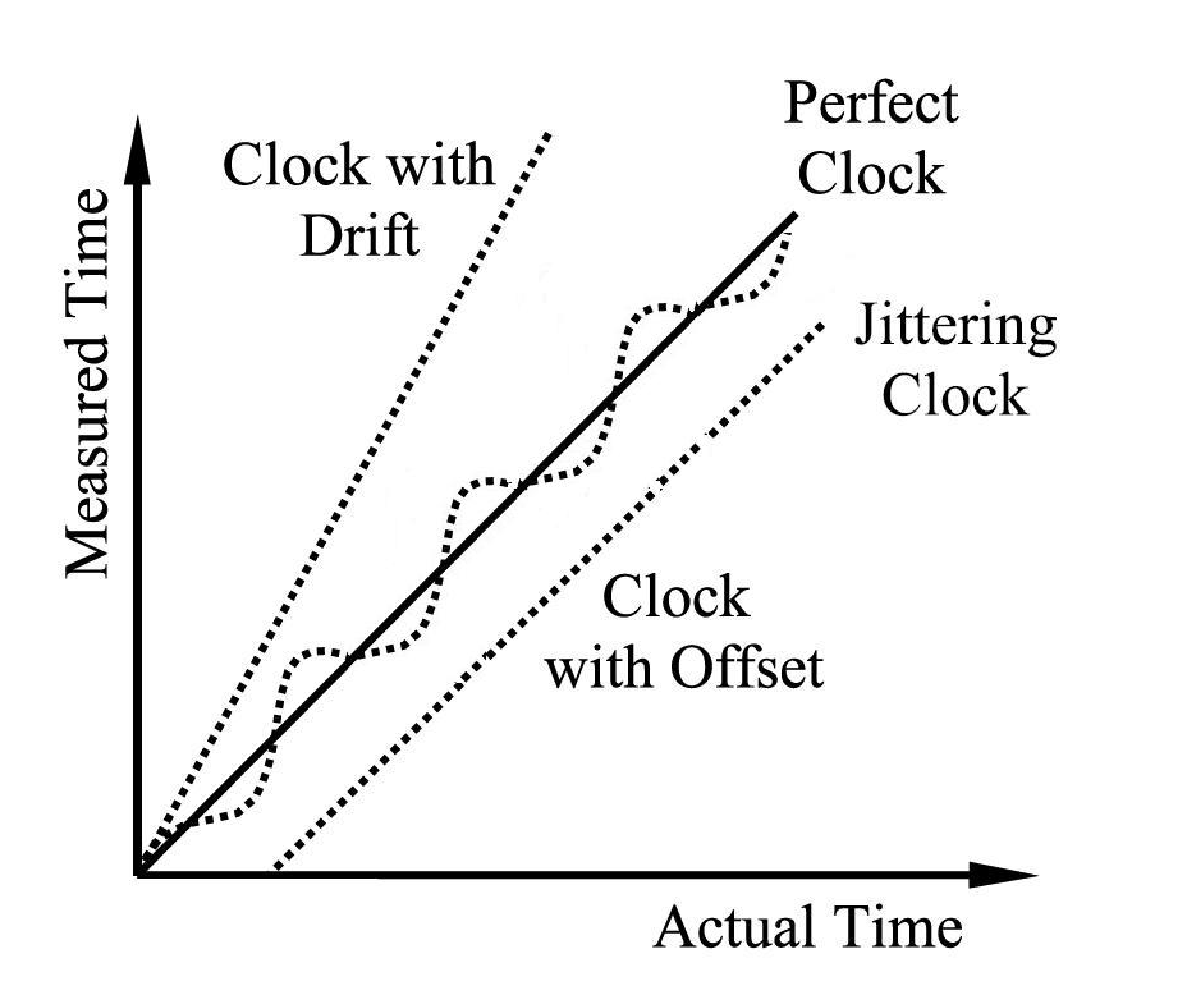
\includegraphics[width=0.5 \textwidth]{actualvsmeasuredtime}
\caption{Measured time versus absolute time} \label{clocktime}
\end{figure}
Note that different clocks have different maximum clock drift values
$\rho$. The frequency of the clock is dependent on many factors and is given$\cite{clockwhite}$ as
\begin{equation}
f_i(t) = f_o + \Delta f + a(t-t_o) + \Delta f_e(t) + \Delta f_n(t)
\label{frequency}
\end{equation}
where \newline $t_o$ = the start time of the clock, \newline $a$ = aging factor, \newline $f_o$ = nominal frequency, \newline $\Delta
f$ = calibration error, \newline $\Delta f_n(t)$ = frequency instability (noise) term,\newline $\Delta f_e$ = frequency error which occurs
due to outside factors such as temperature and voltage instability.\newline
The nominal frequency is the ideal frequency at which the oscillator is supposed to run. Hence, all the above factors affect the value of $\rho$. From ($\ref{clock}$) and ($\ref{frequency}$), we get
\begin{equation}
C_i(t) - C_i(t_o) = \dfrac{1}{f_o} \int^{t}_{t_o}f_i(\tau)d\tau ,
\end{equation}
\begin{equation}
C_i(t) - C_i(t_o) = \dfrac{1}{f_o} \int^{t}_{t_o}{[f_o + \Delta f + a(\tau-t_o)  } + \Delta f_e(\tau) + \Delta f_r(\tau)]d\tau ,
\label{fasika}
\end{equation}
\begin{equation}
C_i(t) =  C_i(t_o) + (t-t_o) +\dfrac{\Delta f}{f_o}(t-t_o) + \dfrac{a}{2f_o}(t-t_o)^2 + \dfrac{1}{f_o}\int^{t}_{t_o}{f_e(\tau)d\tau} +
\dfrac{1}{f_o}\int^{t}_{t_o}{\Delta f_n(\tau)d\tau} .
\label{freqmodel}
\end{equation}
\paragraph*{}
Here are some notes to be considered in the model.
\begin{itemize}
\item The amplitude of the short term variations due to noise $\Delta f_n(t)$ is small enough that they do not cause the clock to accelerate or decelerate in a large amount in the long run.
\item Individual clock properties are uncorrelated.
\item Clock parameters are normally distributed. The variances of the constants in the clock drift equation (initial time error,
initial frequency error, aging rate) are all inputs to the model.
\item The spread in clock time grows almost linearly as a function of time, due to the dominance of the linear term in the clock drift equation.
\end{itemize}
The resulting expression in ($\ref{freqmodel}$) is used to model the clock drift of an oscillator.
\section{\textbf{Building blocks of a synchronization protocol}}
The synchronization protocols can be decomposed into four conceptual building blocks$\cite{taxonomy}$. It is shown in Figure
$\ref{block}$.
\begin{figure}
 \centering
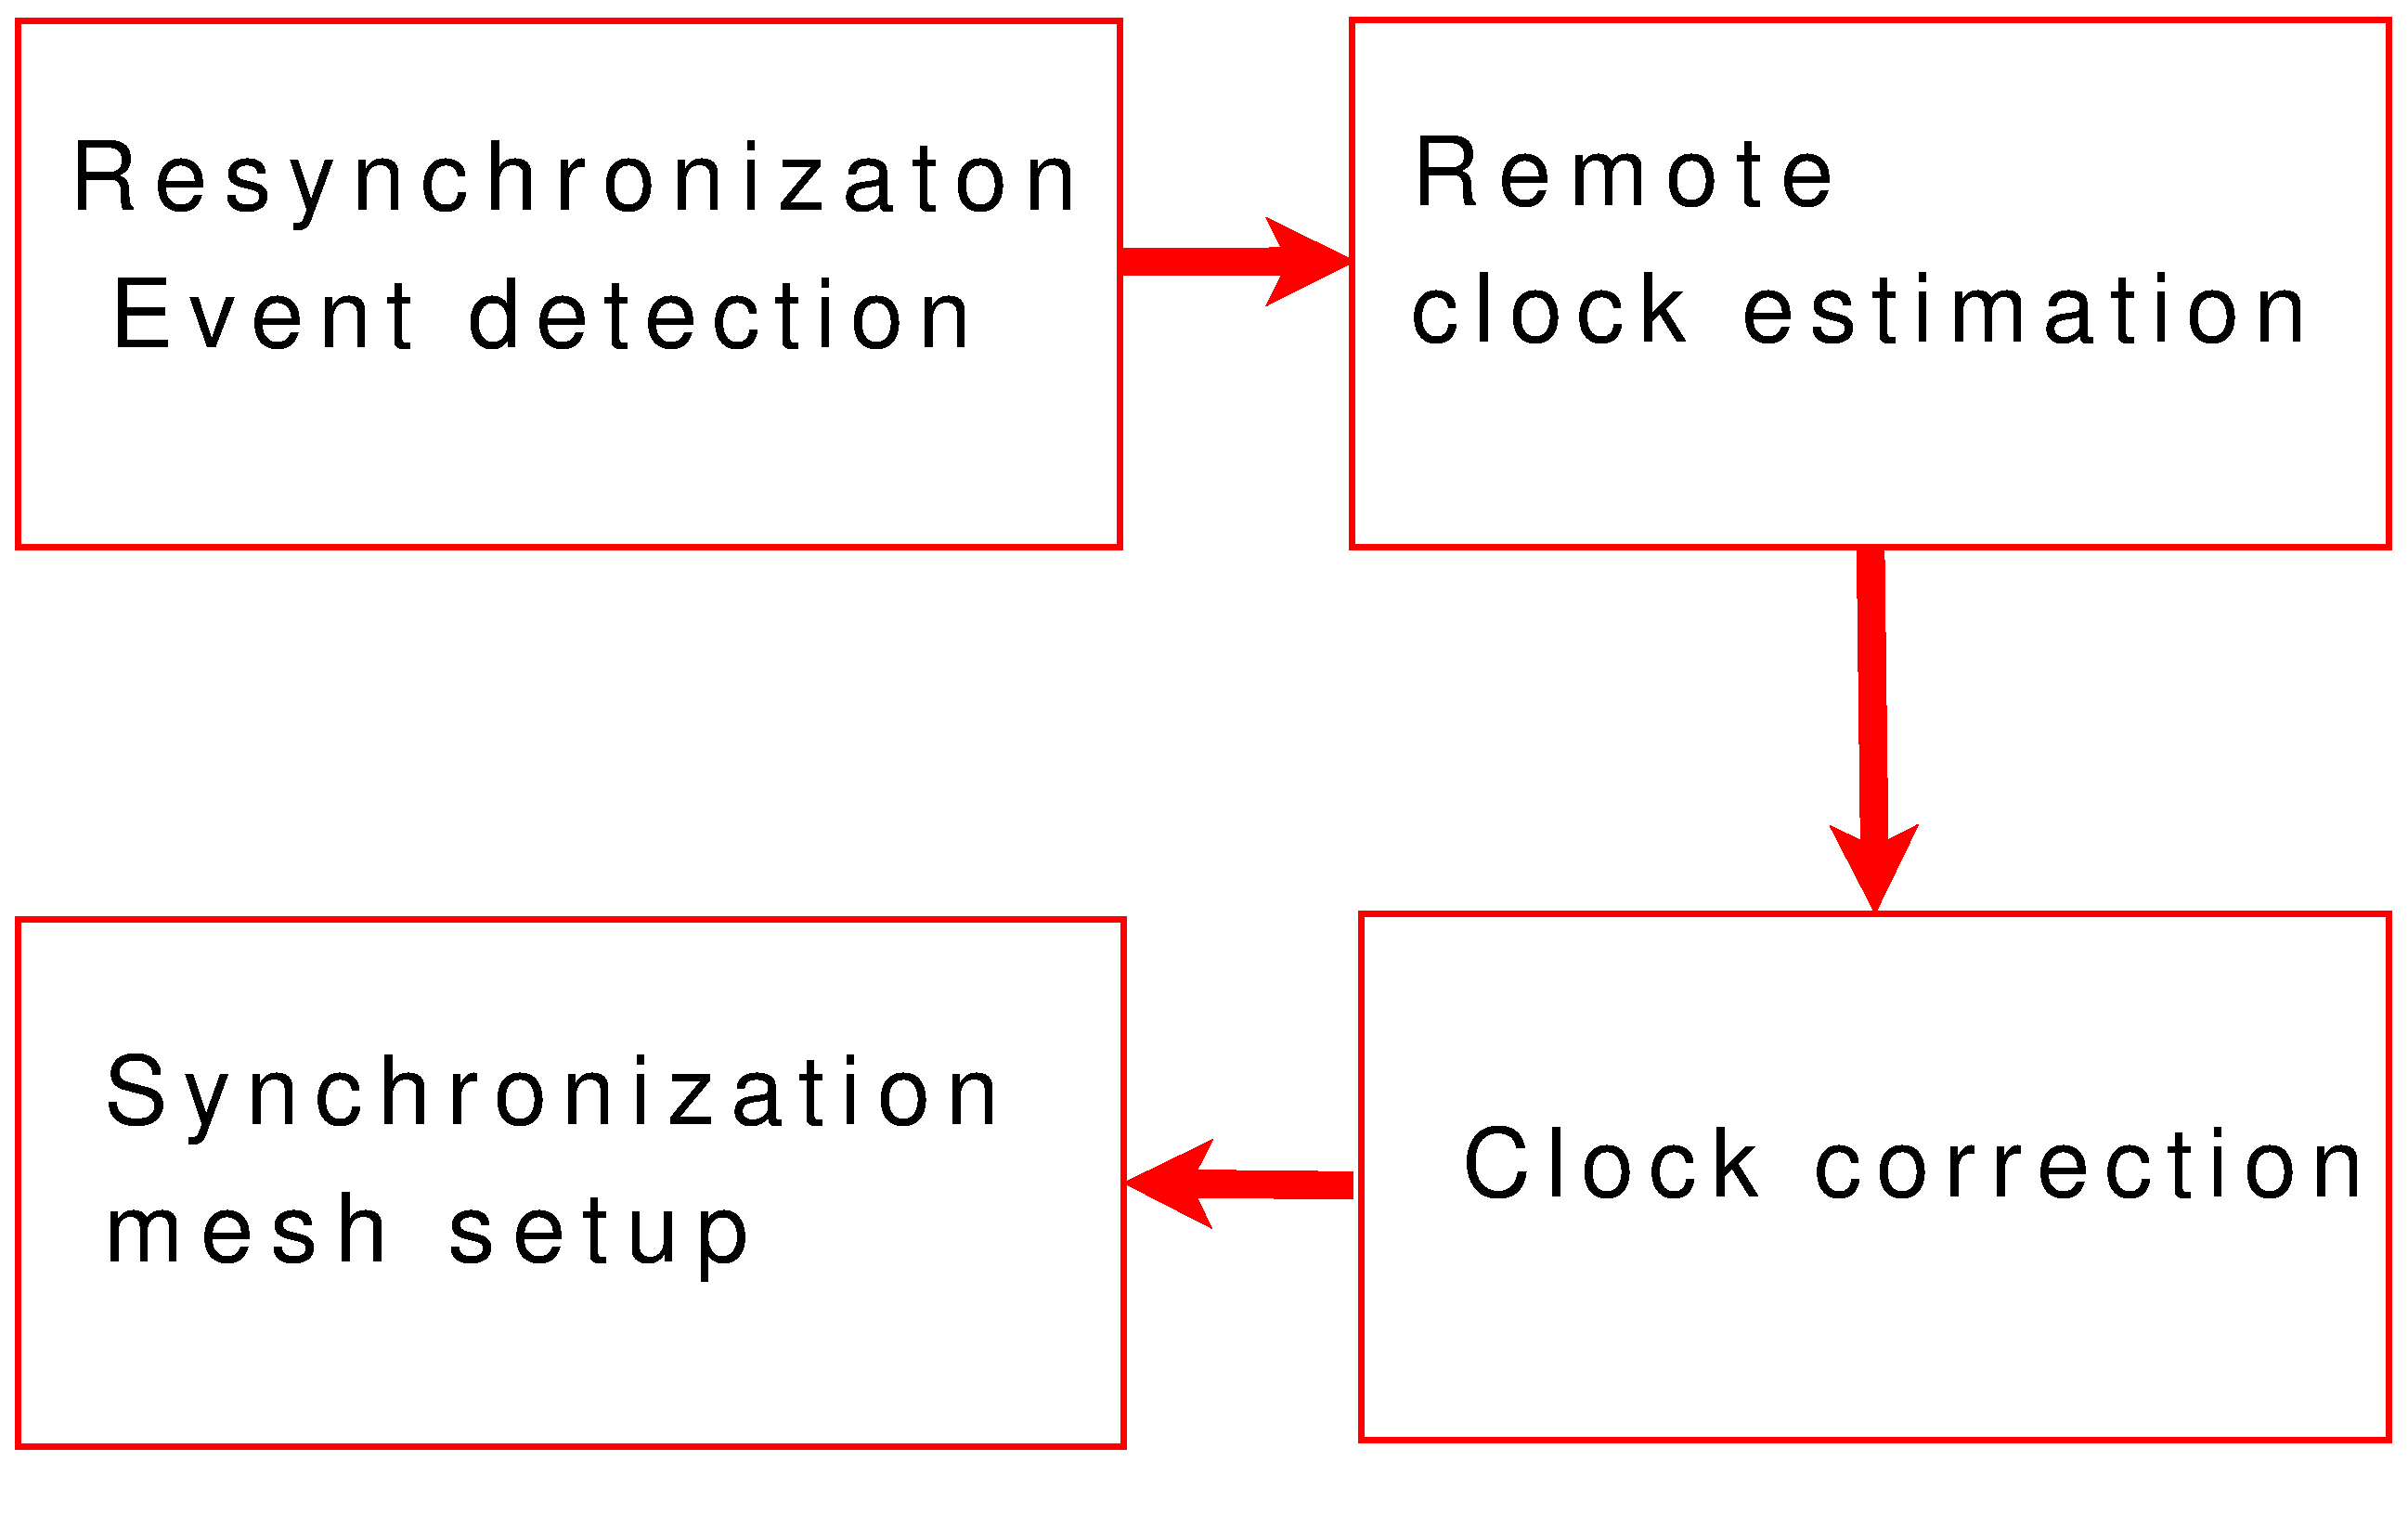
\includegraphics[width= 0.5 \textwidth]{buildingblock}
\caption{Building blocks of a synchronization algorithm}
\label{block}
\end{figure}
\begin{itemize}
\item The resynchronization event detection block identifies the points in time where resynchronization is triggered. A single synchronization process is called a round. If rounds can overlap in time, sequence numbers are needed to distinguish them and to let a node ignore all but the newest resynchronization rounds.
\item The remote clock estimation block acquires clock values from remote nodes/remote clocks.
\item The clock correction block computes adjustments of the local clock based on the results of the remote clock estimating block.
\item The synchronization mesh setup block determines which nodes synchronize with each other in a multihop network. In fully connected networks, this block is trivial.
\end{itemize}
\section{\textbf{Performance metrics of a synchronization protocol}}
There are different metrics in which a synchronization algorithm can be measured. Some of the parameters are discussed below.
\subsubsection{\textbf{Precision}}
Deterministic algorithms guarantee absolute upper bounds on the synchronization error between the nodes or with respect to external time source. In this case, the maximum synchronization error between a node and real time or between two nodes is interesting. For stochastic algorithms (which can only give stochastic bounds in the sense that synchronization error is with some probability smaller than a prescribed bound), the mean error, the error variance or some other quantity is relevant.
\subsubsection{\textbf{Energy costs}}
The energy costs of a time synchronization protocol depend on several factors: the number of packets exchanged in one round of the algorithm, the amount of computation needed to process the packets, and the required synchronization frequency.
\subsubsection{\textbf{Memory requirement}}
To estimate drift rates, a history of previous time synchronization packets is needed. In general, a longer history allows for more accurate estimates at the cost of increased memory consumption.
\subsubsection{\textbf{Fault tolerance}}
How well can the algorithm cope with failing nodes, with error-prone and time-variable communication links, or even with network partitions? Can the algorithm handle mobility?
\section{\textbf{Synchronization frequency}}\paragraph*{}
Decreasing the timing of the synchronization and do periodic execution of the synchronization algorithm greatly reduces
the energy consumption of the wireless sensor network. Thus, a synchronization period, $T_{sync}$, is defined here as the period in which the network can stay synchronized without the application of the synchronization algorithm.
\paragraph*{}
With a synchronization period $T_{sync}$\nomenclature{$T_{sync}$}{Synchronization frequency} and the maximum clock drift of a clock $\rho$ , the maximum time difference between a sender and a receiver is
\begin{equation}
t_{diff} = 2\dfrac{T_{sync}}{T}\rho ,
\end{equation}
where the factor of $2$ reflects the worst case scenario where each node drifts in the opposite direction.
\paragraph*{}
In the implementation of TDMA for communication, a time interval, called guard time $t_{guard}$, is usually left vacant in the beginning and end of a slot during which no data is sent. This time can be used for synchronization and compensating for a signal distortion, as shown in Figure $\ref{guardtime}$. The guard time provides a safety margin against symbol interference in the time between sequential operations such as transmission, encoding, decoding or switching. As the guard time increases, the probability that the message is received in the time slot increases. But in its downturn, it consumes energy as the node is listening throughout this time.
\begin{figure}
\centering
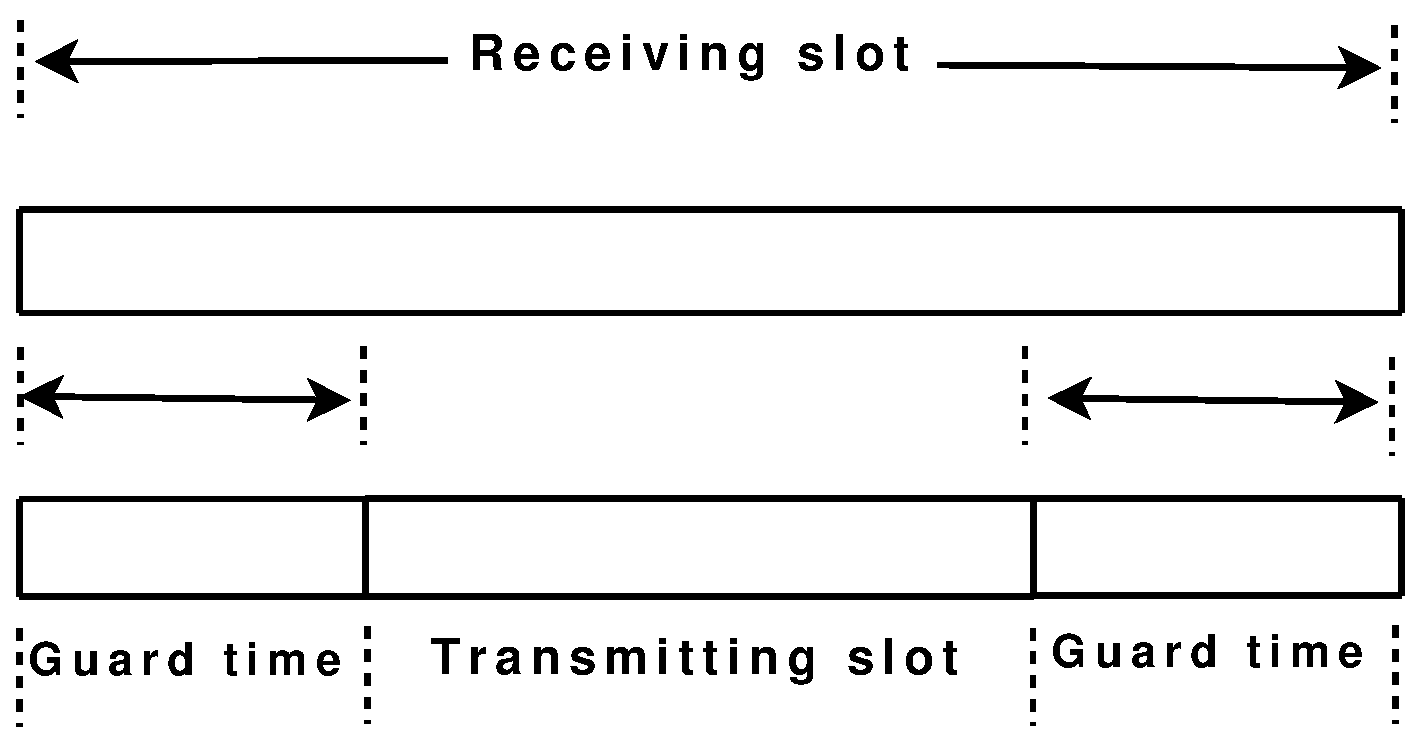
\includegraphics[width=0.5 \textwidth]{guardtime}
\caption{Guard time for drift compensation} \label{guardtime}
\end{figure}
Since the relative time difference between two nodes can be in two direction, the guard time, $t_{guard}$\nomenclature{$t_{guard}$}{Length of the guard time}, needs to be twice $t_{diff}$,
\begin{equation}
t_{guard}= 2t_{diff} = 4\dfrac{T_{sync}}{T}\rho.
\end{equation}
At this end, the minimum duration for a time slot $t_{slot}$\nomenclature{$t_{slot}$}{Time duration of a slot} is
\begin{equation}
t_{slot} \geq t_{guard} + T_{tx},
\end{equation}
where $T_{tx}$ is a system constant and it represents the required time to send a packet from one node to other. Two nodes have a good communication link when they synchronize their clocks at least once every $T_{sync}$ that gives the following
relation,
\begin{equation}
\dfrac{T_{sync}}{T}\geq 1.
\end{equation}
It is a good practice to design systems having a $T_{sync}$ greater than the time frame. It increases the battery life of a node. However,
this has a negative impact on the performance of the network.
\paragraph*{}
To obtain the value of $T_{sync}$ for a particular system with a given duty cycle, the following are considered
\begin{equation}
t_{guard} \geq 4\rho \dfrac{T_{sync}}{T}
\end{equation}
\begin{equation}
t_{slot} \geq t_{guard} + T_{tx}
\end{equation}
\begin{equation}
\dfrac{T_{sync}}{T} \geq 1
\end{equation}
Hence, there is a trade-off in determining $T_{sync}$: increasing $T_{sync}$ reduces the energy costs of synchronization, but decreases the network perfromance. This is because the synchronization done less frequently so than nodes might drift out of synchronization in the mean time.
\section{\textbf{Median algorithm and the flaw}} As stated earlier, the Median algorithm is currently implemented in the MyriaNode. With the simplicity concerning the computational need, the Median algorithm is the best fit for the energy requirment. The algorithm is described as follows:
\begin{enumerate}
\item Nodes broadcast packets.
\item Each receiver records the time that the packet is received according to the local clock.
\item Each receiver $i$ computes its phase error to any other node $j$ in the neighborhood,
\begin{equation}
\Delta t_{ij}^{(n)} = t_i^{(n)} - t_j^{(n)} , \label{pha}
\end{equation}
where $t_i$ is the wakeup time of node $i$ and $t_j$ is the wakeup
time of node $j$ at the $n^{th}$ period.
\item Receivers compute the offset, $\xi_i$, to be the median of the phase errors,
\begin{equation}
\xi_i^{(n)} = median(\Delta t_{ij}^{(n)}) , \forall j
\end{equation}
\item Receivers adjust their wakeup time by the computed offset value,
\begin{equation}
t_{i}^{(n+1)} = t_i^{(n)} + T_i^{(n)} - G\xi_i^{(n)},
\end{equation}
\end{enumerate}
\begin{figure}
\centering
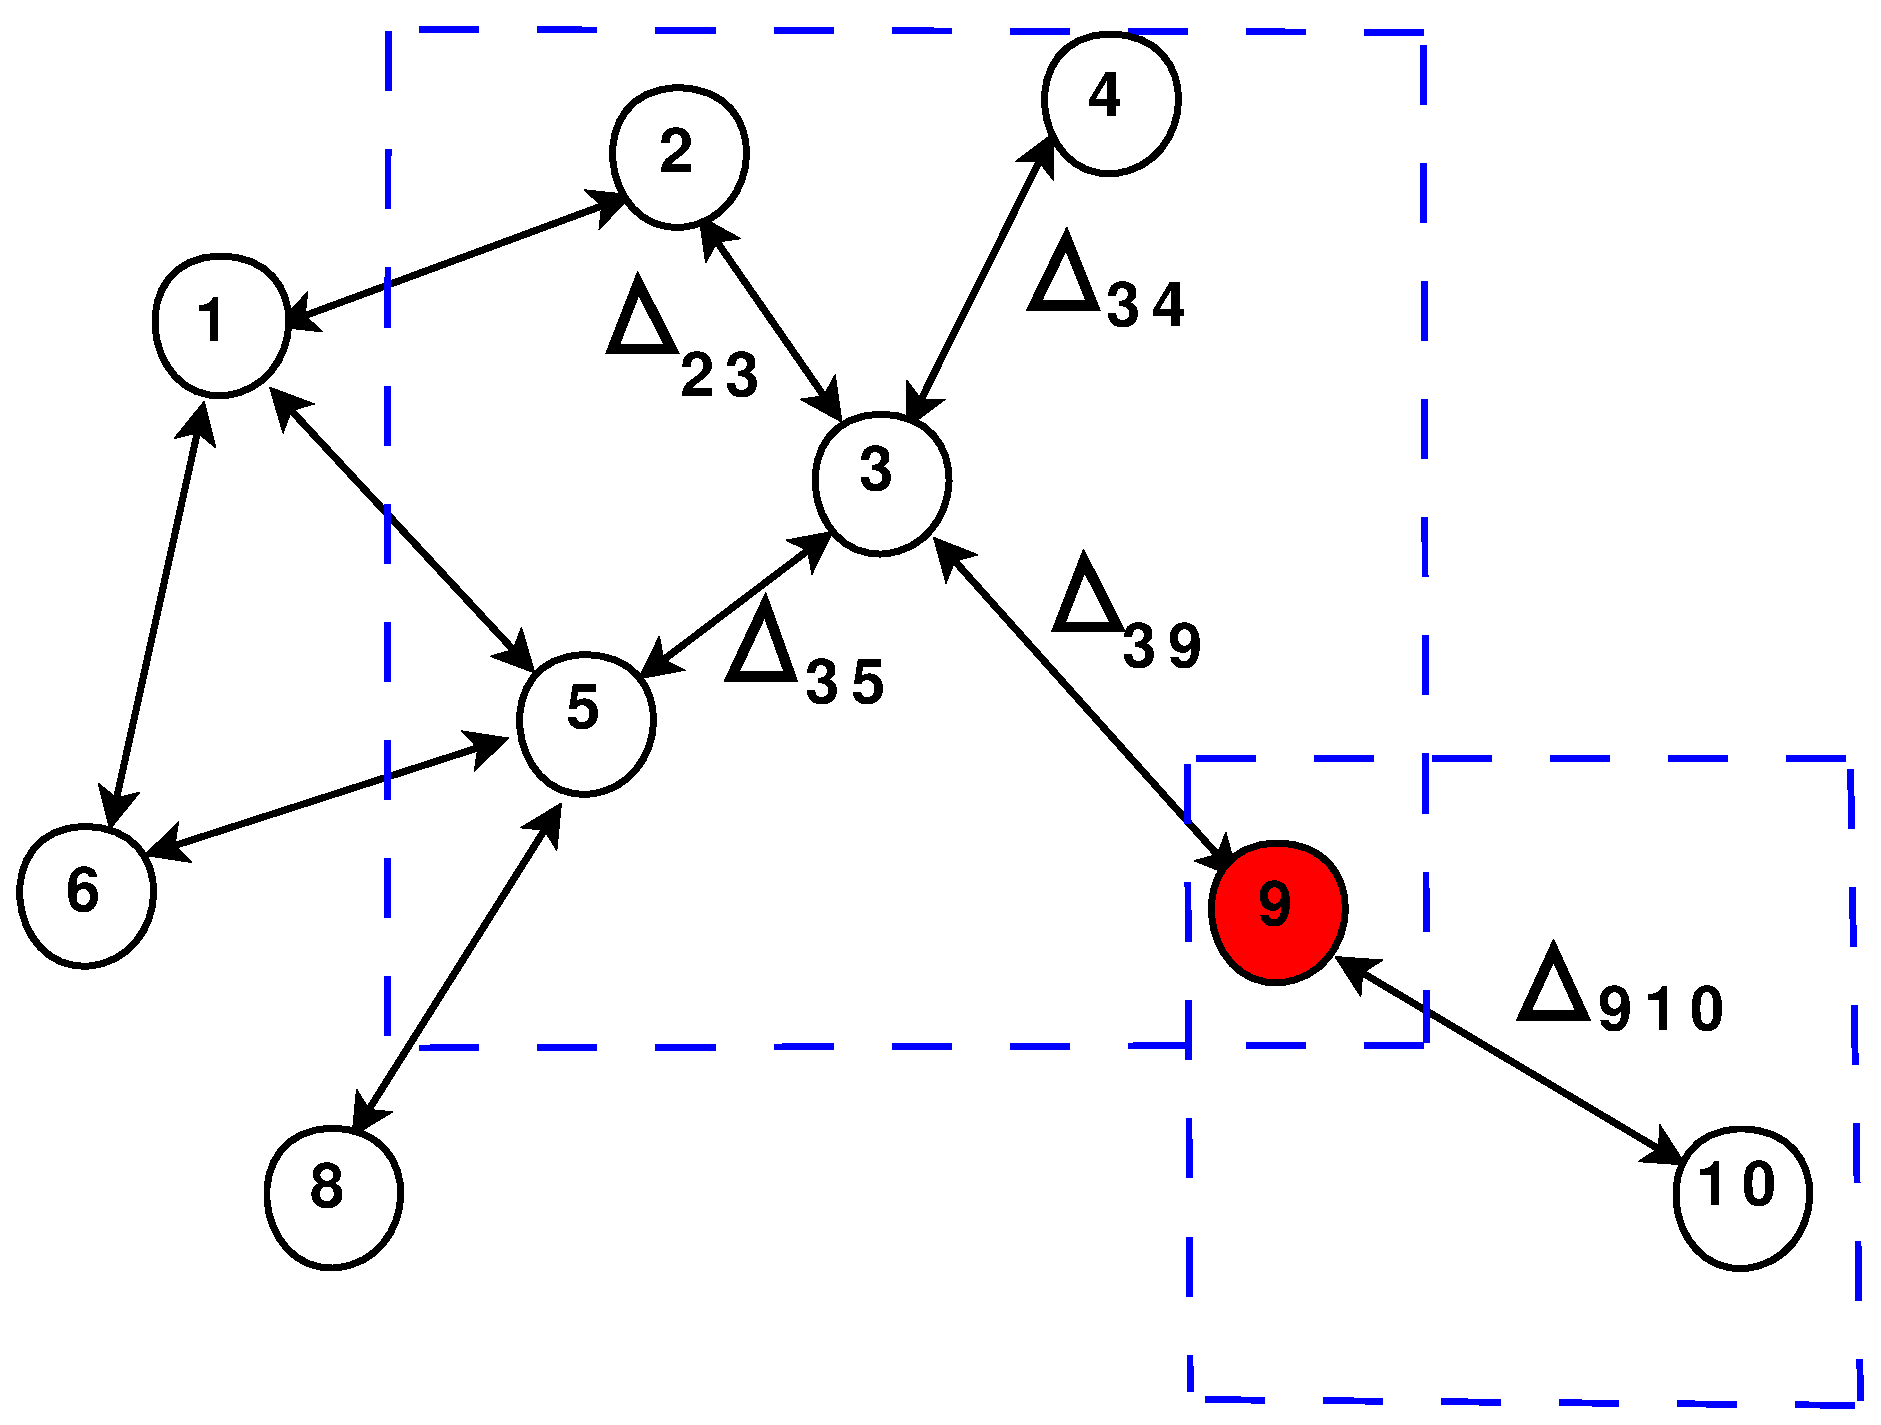
\includegraphics[width=0.5 \textwidth]{node_field}
\caption{A WSN scenario} \label{wsn}
\end{figure}
where $G$ is the \textit{gain factor}. By multiplying the median with a gain factor, i.e. $G\xi_i^{(n)}$, the output can be adjusted for better performance. Hence a gain factor is added to ensure better precision of the synchronization error.
\newline
As per the application of Median, there are flaws on its implementation. In some test-cases, the algorithm fails to converge or stays unsynchronized for a certain period of time. This results in a  communication disruption in places where synchronization is essential.
\paragraph*{} A typical scenario is presented where the Median algorithm takes a longer time to achieve synchronization. In Figure
$\ref{wsn}$, a distribution of wireless sensor nodes is shown. Node 10 joins the stable network communication through Node 9. Assume Node 9 belongs to two broadcast domains, Node 3's and Node 10's. Thus, upon the application of the median algorithm, the node tends to
adjust its wakeup time with the median of the offsets from its neighbors, Node 3 and Node 10. Adjusting the wakeup time, the offset to be is
\begin{equation}
\xi_9 = median(\Delta t_{9,10} , \Delta t_{9,3}).
\end{equation}
With Node 10 being isolated from the well established network, it has a major drift from the other nodes. Being in synchronization
with the other nodes, Node 9 will drift away from the network after its adjustment with Node 10. Due to the adjustment, tt will take Node 9 more time to synchronize with the network again. Therefore, the performance of the median algorithm decreases with the increase in the dynamic nature of the network. Figure $\ref{fasik}$ shows the state of the network after the synchronization using the Median. Node 9 has drifted away from the networks in order to incorporate the effect of the new neighbor Node 10.
\begin{figure}
\centering
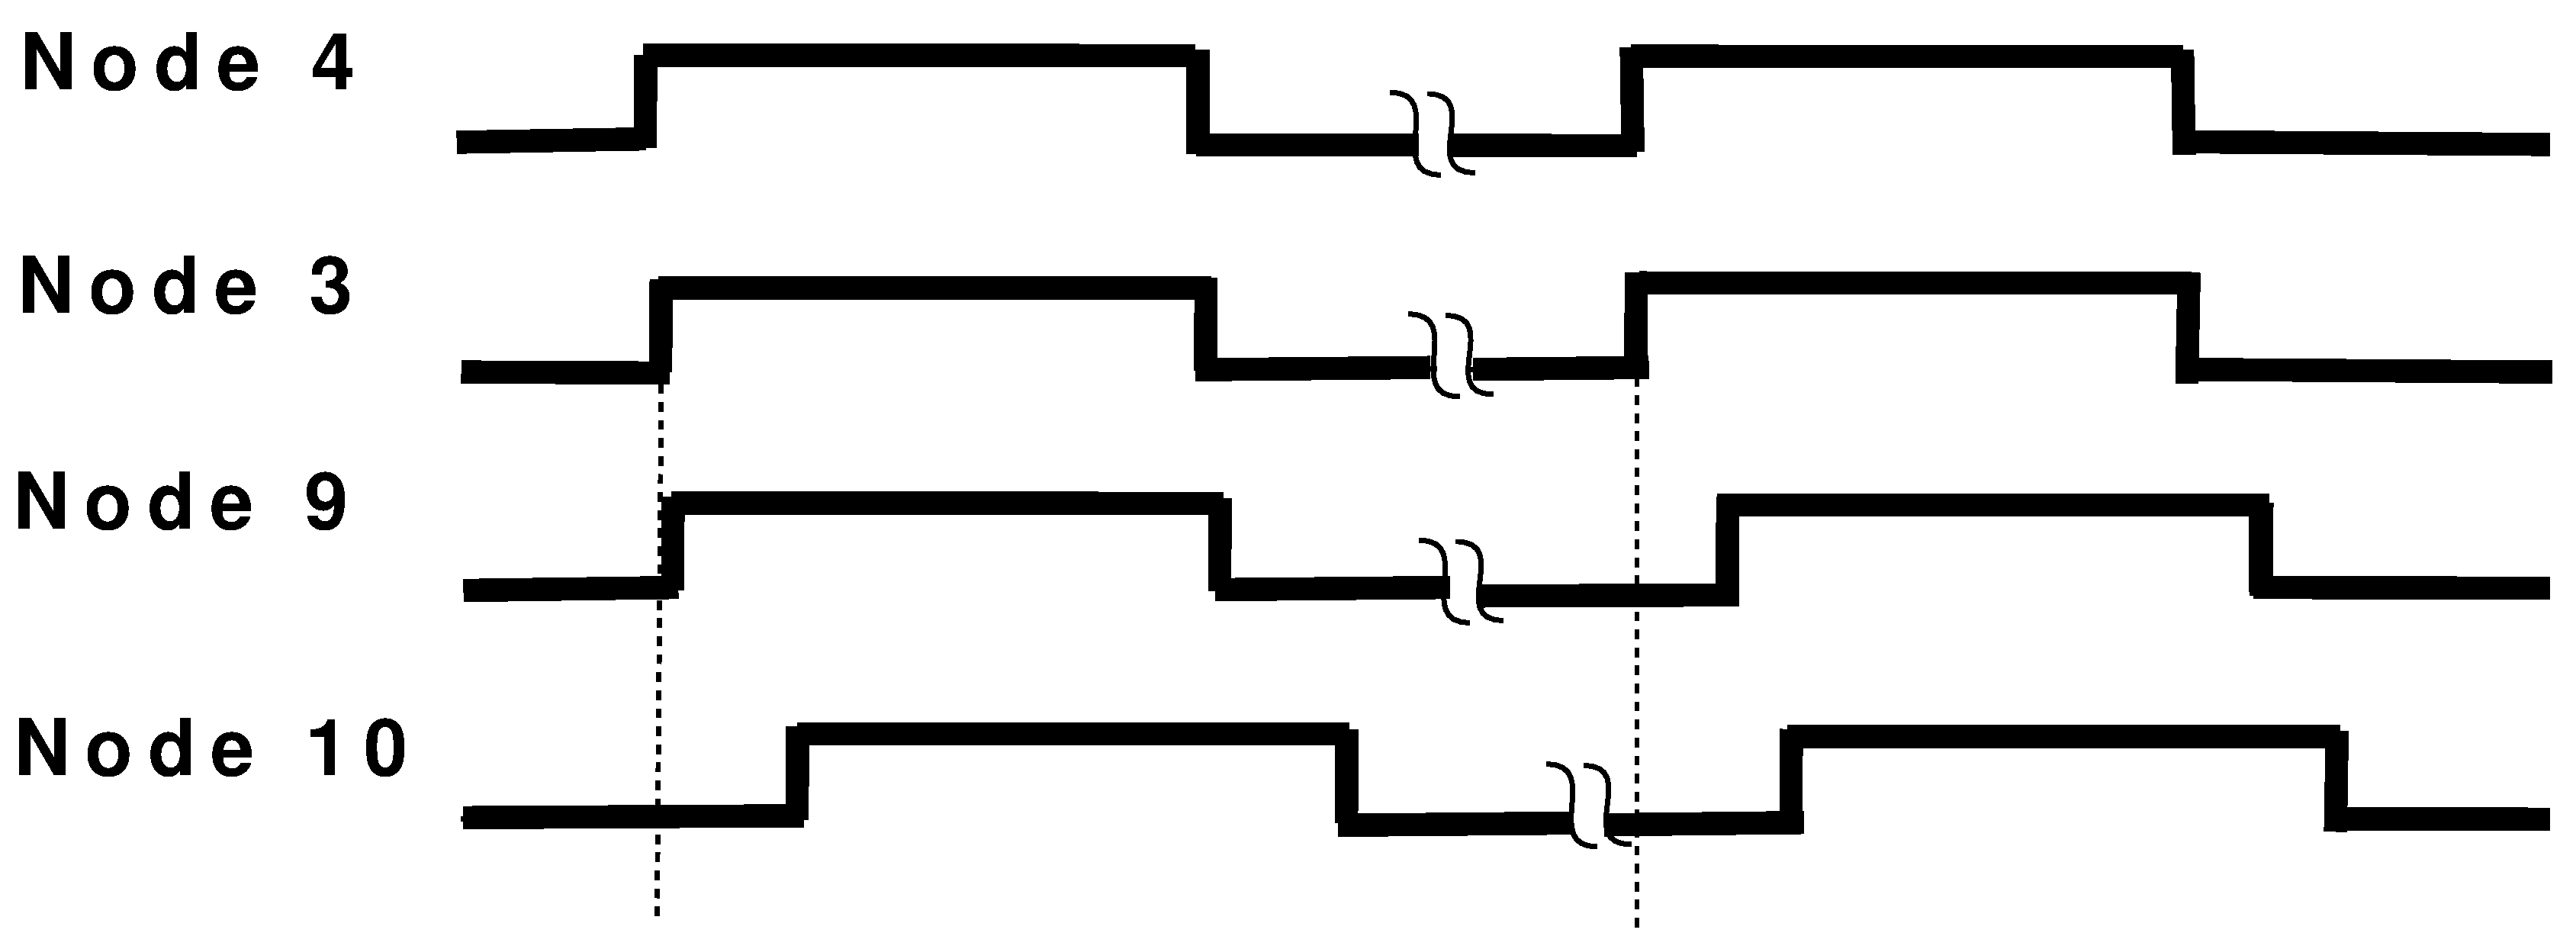
\includegraphics[width= 0.5\textwidth]{offsetpic}
\caption{Using median for phase error correction} \label{fasik}
\end{figure}
\paragraph*{}
So, in order to address this problem, three algorithms are proposed to realize an energy-efficient, more precise and simple frame synchronization. The algorithms are explained in the next chapter.
\chapter{\textbf{Synchronicity protocol}}
\section{\textbf{Mathematical model}}
As part of the message, the nodes send the slot number which they are transmitting to the neighbours. This information is used in determining the time that the message is sent. This information is used in determining the time that the message is sent. Each message that is sent withtin a slot is received by a neighbor at a known clock tick number, $tick_{rx}$, as
\begin{equation}
tick_{rx} = T_{tx}+ \dfrac{t_{guard}}{2}, \label{tick}
\end{equation}
where $t_{guard}$ is the guard time and $T_{tx}$ is the transmission time of a packet. \newline
Whenever ($\ref{tick}$) is not satisfied, a phase error is observed. The wakeup time of a node at a random time after $n$ periods of firings since it is turned on is
\begin{equation}
t_i^{(n)} = \sum_{n} T_i^{(n)} + t_{io},\label{newphase}
\end{equation}
where  $T_i^{(n)}$ is the period of the crystal clock at the $n^{th}$ period since it changes with time according to
($\ref{frequency}$) and $t_{io}$ is the initial start-up time of the node. The frequency of the node varies due to the different factors mentioned in ($\ref{frequency}$). \paragraph*{}
Substituting ($\ref{newphase}$) in ($\ref{pha}$), the difference in the wakeup time of the nodes will be
\begin{eqnarray}
\Delta t_{ij} & = & \sum_{n}T_i^{(n)} + t_{io}- (\sum_{n}T_j^{(n)} +
t_{jo}) \\ &=& (\sum_{n}T_i^{(n)} - \sum_{n}T_j^{(n)}) +
(t_{io}-t_{jo}).
\end{eqnarray}
The offset being applied should be able to compensate for the phase error introduced by the drift as well as the frequency changes. This can be done by adjusting the next wakeup time depending on the difference between the current wakeup time of the node and its neighbors. Application of offset compensating using prediction of the next wake up time is the promising approach to be implemented on the MyriaNode. The next wakeup time of the node is dependent on the current wakeup time of its neighbors in relation to its previous wakeup time,
\begin{equation}
t_i^{(n+1)} = t_i^{(n)} + T_i^{(n)} - \xi_i^{(n)} ,
\end{equation}
where $T_i$ is the period of the node's clock and $\xi_i$\nomenclature{$\xi_i$}{Offset to be added to Node $i$'s wakeup time} is given by
\begin{equation}
\xi_i = f(\Delta t_{ij}).
\end{equation}
The function $f$ is based on an algorithm which takes the wakeup time differences between the node and its neighbors and determines
the optimal offset to be added to the next wakeup time of the node.
\newline Different algorithms are presented here and discussed with the simulation results presented in the next chapter of the report.
\subsection{\textbf{Weighted measurements}}
One form of approach to tackle the dynamic behavior of a WSN is a Weighted Measurements (WM) approach. Using this approach, different weights are given to the different phase errors. A weight is added to increase the influence of the close by neighbors and ensure faster synchronization. In addition to that, a new joining neighbor can get synchronized with out disturbing the existing neighbors, adjusting its time to the big swarm of nodes. \paragraph*{}
The offset, $\xi_i$, is calculted as
\begin{equation}
\xi_i^{(n)} = \sum{w_{ij}^{(n)}\Delta t_{ij}^{(n)}} ,
\end{equation}
where $\sum{w_{ij}^{(n)}= 1}$ and $w_{ij}$ is the weight factor for the phase error $\Delta t_{ij}$ and $n$ is the number of periods that passed since the node is turned on.
\paragraph*{}
The weighted adjustment is used to modify the next wakeup time of the node,
\begin{eqnarray*}
t_i^{(n+1)} &=& t_i^{(n)} + T_i^{(n)} - \xi_i^{(n)} \\ &=& t_i^{(n)}
+ T_i^{(n)} - \sum_{j=0}^N{w_{ij}^{(n)}\Delta t_{ij}^{(n)}} \\ &=&
t_i^{(n)}+ T_i^{(n)} -
\sum_{j=0}^N{w_{ij}^{(n)}(t_i^{(n)}-t_j^{(n)})} \\ &=& T_i^{(n)} + \sum_{j=0}^N{w_{ij}^{(n)}t_j^{(n)}}.
\end{eqnarray*}
The main task in this algorithm is how to choose the weight factors so that the stability of the network (timewise) is achieved faster. In the selection of the weight factor, two steps are taken. \paragraph*{} \noindent
Firstly, each phase error $\Delta t_{ij}$ is associated with a pre-weight factor, $\delta_{ij}$. $\delta_{ij}$ is used to weigh how far the neighbor nodes has drifted. The $\delta$ values are calculated as:
\begin{equation}
\delta_{ij} = ae^{-b\Delta t_{ij}}.
\end{equation}
\begin{figure}[t]
\centering
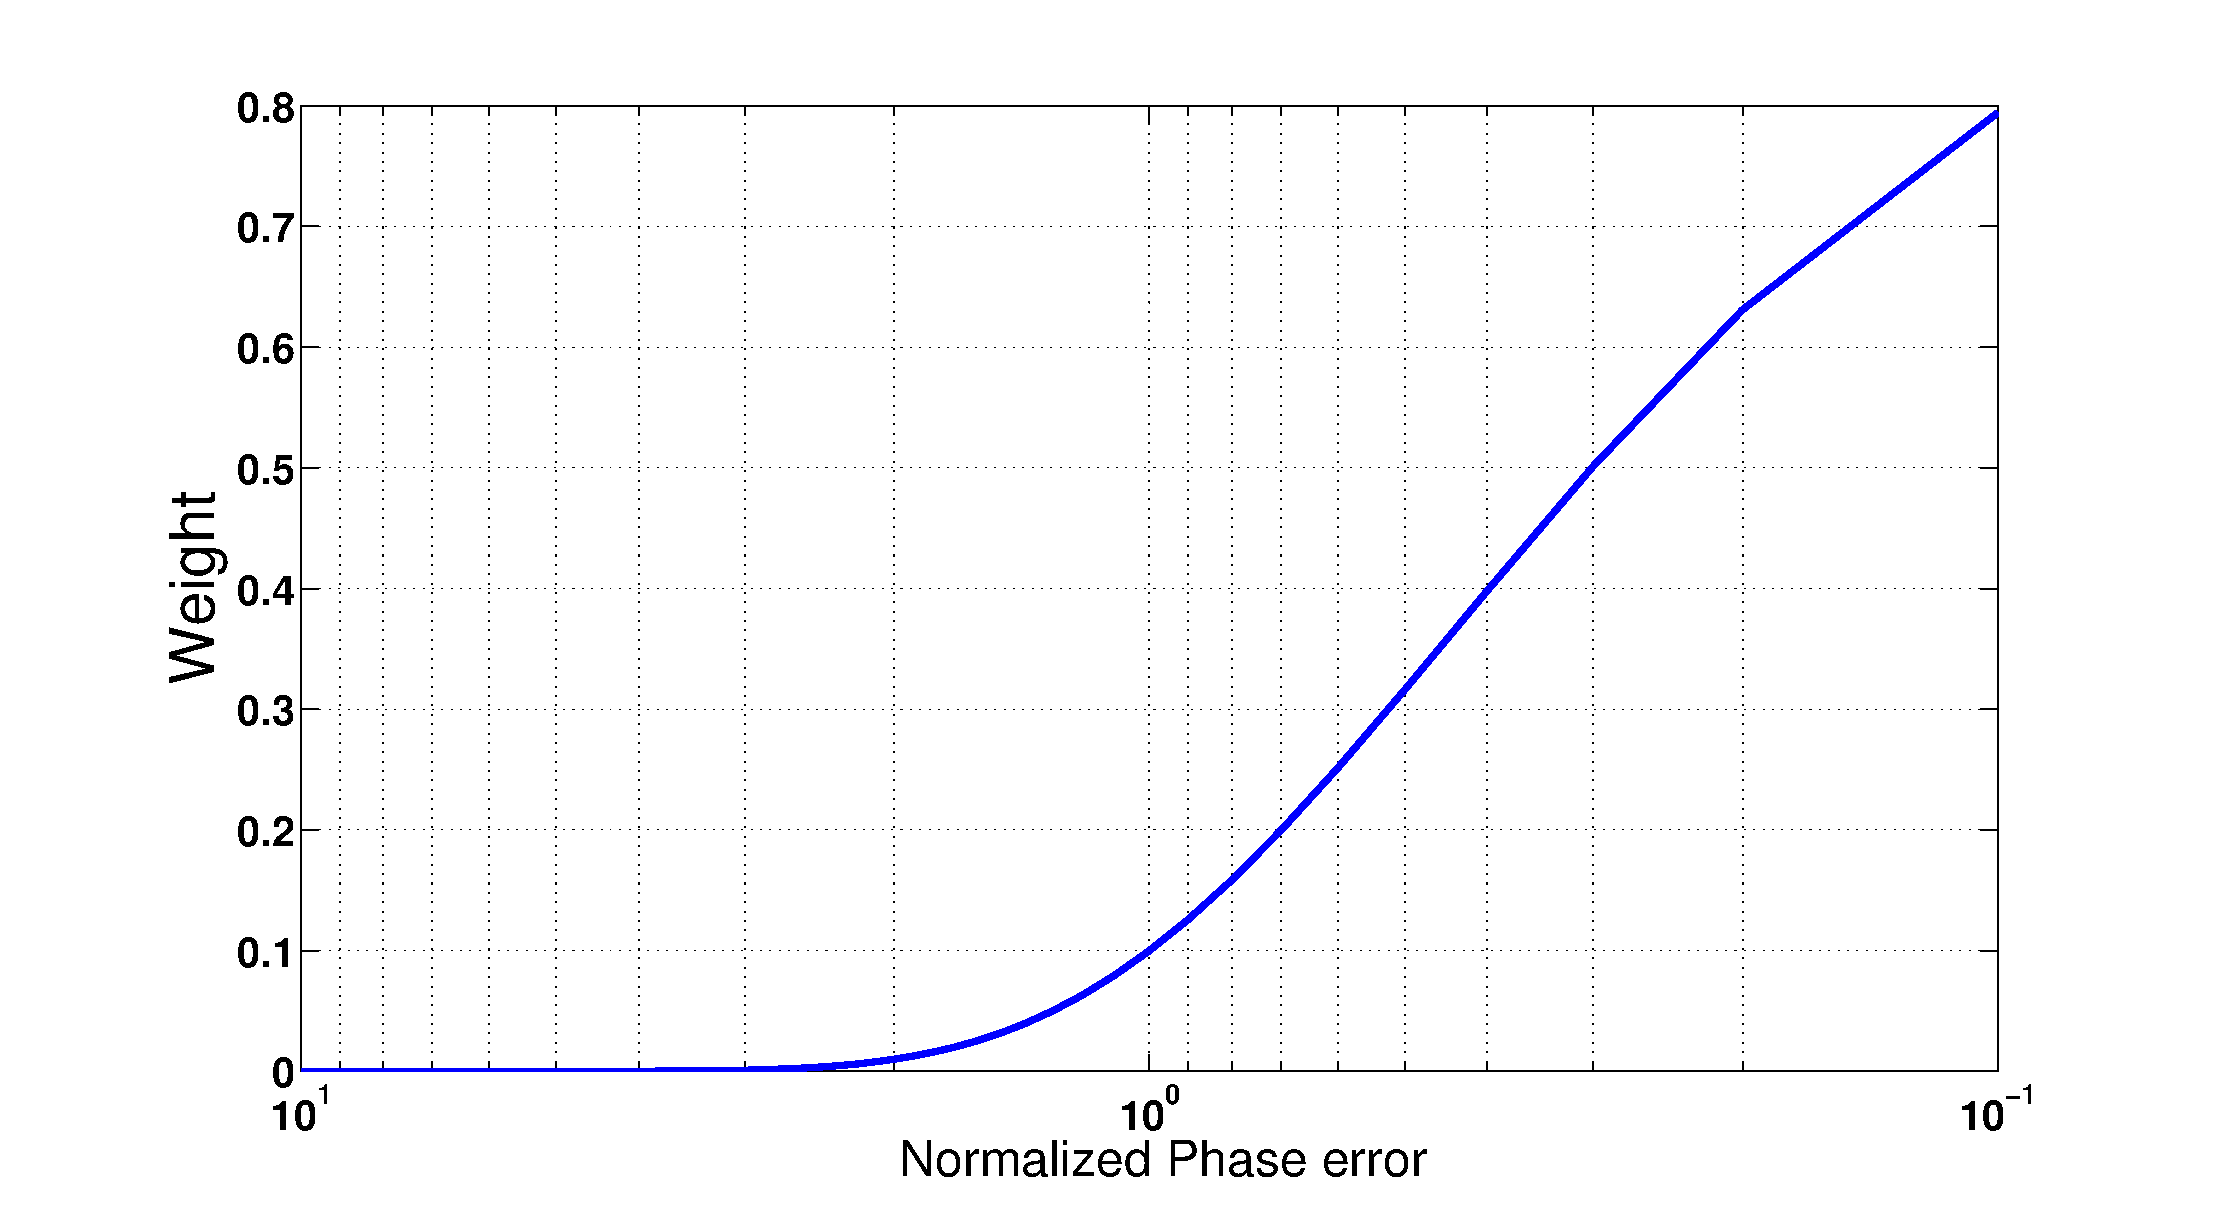
\includegraphics[width= 0.6\textwidth]{weightphase}
\caption{pre-Weight factors for the phase error distribution}
\label{weight}
\end{figure}
The parameters $a$ and $b$ are selected using the initial conditions, $\delta_{ij}=0.1$ for $\Delta t_{ij}$ = $\dfrac{t_{guard}}{2}$ and $\delta_{ij}=1$ for $\Delta t_{ij}$ = 0. As shown in Figure $\ref{weight}$, the closer the phase error is to zero, the higher value of pre-weight $\delta$ is given to the phase error. The assignment of high values to small phase errors will decrease the time it takes to synchronize the node with the closby neighbours than the rest.
\paragraph*{} \noindent
Secondly, the weight factor is calculated based on the distribution of the assigned pre-weight factors $\delta$ for each phase error. If all or most of the phase errors are small, this corresponds to the fact that the node has drifted away from most of the neighbours. Hence, the synchroniztion is made to adjust the nodes wakeup time towards the neghbours. \paragraph*{} \noindent
Hence, the weight factor is
\[w_{ij} = \left\{
\begin{array}{l l}
  1 - \delta_{ij},& \quad \mbox{if $mean(\delta_{ij}$) $<$ 0.5}\\
 \delta_{ij}, & \quad \mbox{if $mean(\delta_{ij}$) $>$ 0.5}\\ \end{array} \right. \]
where $mean$ is the average function.
The weight then moves towards the large phase errors if the node is a new-comer that wants to join the "already established" network.
\paragraph*{}
Therefore, in WM approach, the first step describes how the node has drifted away from its neighbors whereas the second one describes how the node is positioned in the time topology which surrounds it. Using the WM approach, a series of measurements will be used to estimate the next wakeup time of the node, giving less value/emphasis to the nodes which are out of reach from the neighboring nodes. The simulation result is shown in the next section to see the effect of the algorithm in comparison to the other proposed algorithms.\paragraph*{}
\begin{tabular}{  l }Algorithm for WM \\\hline \hline
1. Nodes broadcast packets. \\  2. Each receiver records the time that the packet is received with respect to the local clock. \\
3. Each receiver i computes its phase error to any other node j in the neighborhood. \\
4. Each receiver i computes the pre-weight factors for the corresponding phase errors. \\
5. Each receiver i computes the weight factor for each pre-weight factors. \\
6. Each receiver i computes the offset using the weight factor method. \\
7. Each receiver adjusts its wakeup time using the offset calculated.\\
\hline \hline
\end{tabular}
\subsection{\textbf{Non linear least squares method}}
\subsubsection{Non linear Least squares}
Non Linear Least Squares (NLLS) is a method to fit a set of $n$ observations with a model that is non-linear in $m$ unknown parameters by minimizing the sum of the squares of the errors ("the residuals"). It uses a set of $n$ data points which are ($x_1$, $y_1$), ($x_2$, $y_2$),$\dots$,($x_n$, $y_n$), and a curve (model function) $y= f(x, \beta)$, that in addition to the variable $x$ also depends on $m$ parameters($\beta_1,\beta_2,...,\beta_m$).
It is desired to find the vector $\beta$ of parameters such that the curve best fits the given data in the least squares, that is, the sum of squares
\begin{equation}
    S=\sum_{i=1}^{n}r_i^2 ,
\end{equation}
is minimized, where the residuals $r_i$ are given by
\begin{equation}
    r_i = y_i - f(x_i,\beta),
\end{equation}
for i=1,2,$\dots$, $n$.
\paragraph*{}
The minimum value of $S$ occurs when the gradient is zero. Hence, there are $m$ gradient equations to be solved:
\begin{equation}
    \dfrac{\partial S}{\partial \beta_j}=2\sum_i r_i\dfrac{\partial r_i}{\partial \beta_j}=0 \ \quad for \quad j=1,2...,m.
\end{equation}
In a non-linear system, the derivatives $\dfrac{\partial r_i}{\partial \beta_j}$ are functions of both the independent variable and the parameters. These gradient equations do not have a closed solution. Instead, initial values must be chosen for the
parameters. Then, the parameters are refined iteratively, that is, the values are obtained by successive approximation,
\begin{equation}
    \beta_j^{p+1}=\beta^p_j+\Delta \beta_j,
\end{equation}
for $j=1,2...,m.$. Here, $p$ is an iteration number and the vector of increments, $\Delta \beta_j$, is known as the shift vector. At each iteration, the model is linearized by approximation to a first-order Taylor series expansion about $\beta^p$.
\begin{equation}
    f(x_i,\beta)\approx f(x_i,\beta^p) +\sum_j \dfrac{\partial f(x_i, \beta^p)}{\partial \beta_j} \left(\beta^p_j -\beta_j \right)
\end{equation}
\begin{equation}
 f(x_i,\beta) =f(x_i, \beta^p)+\sum_j J_{ij} \Delta\beta_j.
\end{equation}
The Jacobian, $J$, is a function of constants, the independent variable and the parameters. So it changes from one iteration to the
next. Thus, in terms of the linearized model,
\begin{equation}
\dfrac{\partial r_i}{\partial \beta_j}=-J_{ij}
\end{equation}
and the residuals are given by
\begin{equation}
    r_i=\Delta y_i- \sum_{j=1}^{m} J_{ij}\Delta\beta_j,
\end{equation}
where
\begin{equation}
 \Delta y_i=y_i- f(x_i, \beta^p).
\end{equation}
Substituting these expressions into the gradient equations and equating to $0$, the resulting system of equations can be represented as a matrix notation as
\begin{equation}
    \left(J^TJ\right)\Delta  \beta=J^T\Delta y.
\end{equation}
\subsubsection{Model design}
As the algorithm is decentralized, the next wakeup time of the node depends on the current phase errors that it has with the other nodes. The distribution of the phase error is the crucial factor in deciding the type of curve to fit in. The phase errors shows how many time units that the neighbor node is out of touch with the node in focus. The larger the phase error is, the more out-of-sync the node is.\paragraph*{}
The set of data are the measured phase errors of the node with its neighbors. In order to meet the demand of adjusting the time offset and stabilize the network, the logarithmic curve with the model
\begin{equation}
 f(x_i,\beta)= \beta _1 + \beta_2log(x_i),
\end{equation}
is chosen. \paragraph*{}
A logarithmic function can be used to represent the distribution of the offsets in the neighborhood, as shown in Figure $\ref{curvefit}$. As shown in the figure, the phase errors are distributed (in an increasing order) so that the maximum phase error will be $\dfrac{t_{guard}}{2}$. Normalized phase error values tend to be small and follow a curve in such away that the maximum value of the phase error should not be greater than guard time.
\begin{figure}
\centering
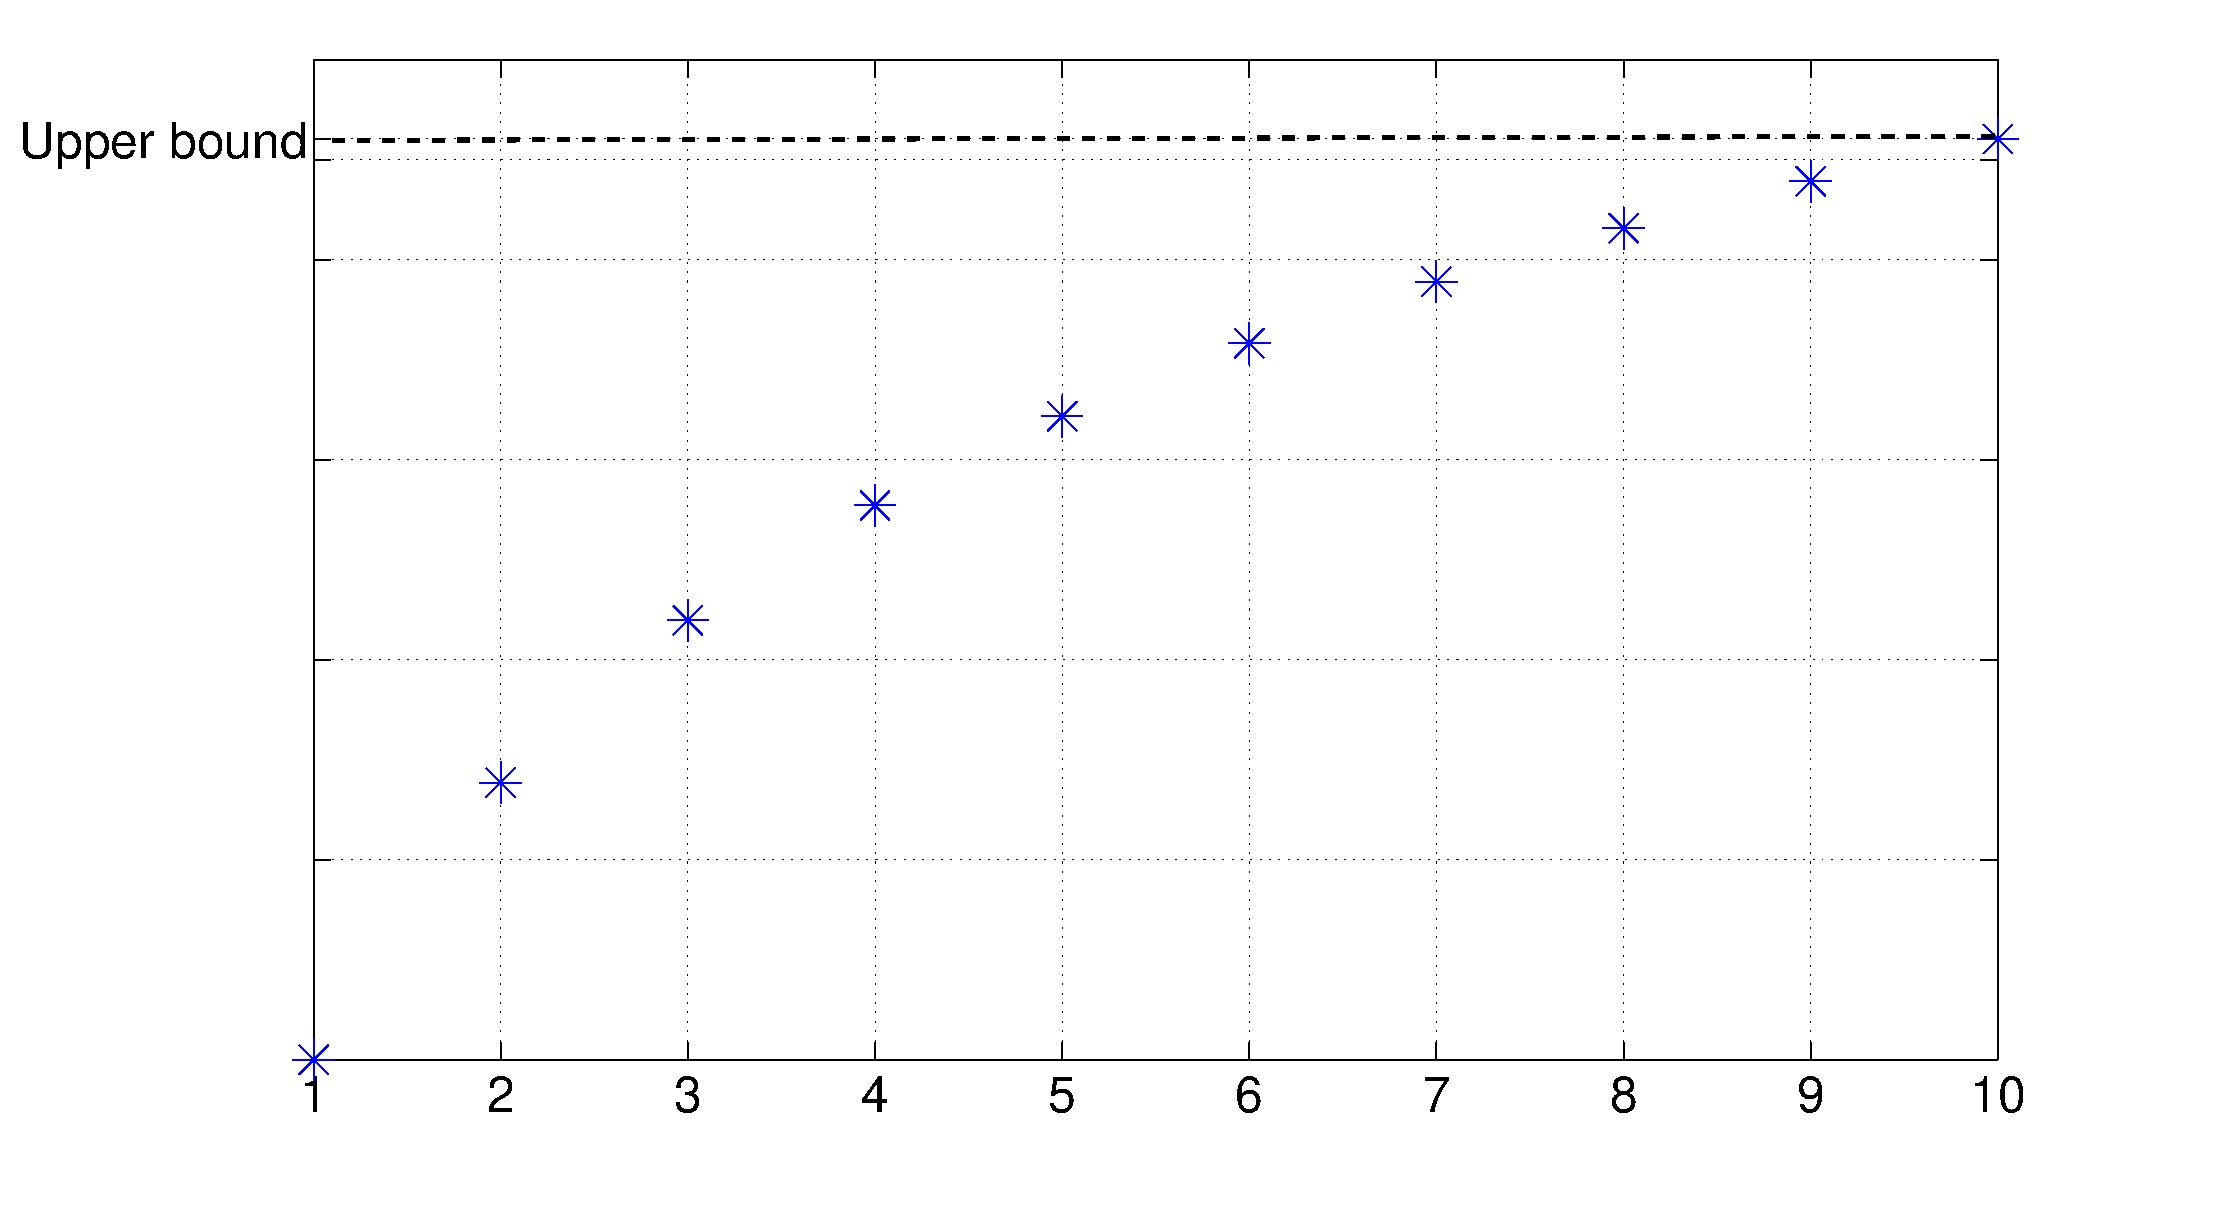
\includegraphics[width= 0.6 \textwidth]{curvefit}
\caption{Curve fitting using logarithmic function} \label{curvefit}
\end{figure}
\paragraph*{}
The initial values of the parameters $\beta_1$ and $\beta_2$ is estimated taking into account the state of a synchronized network, which means $f(0)=0$ and $f(n-1)=\dfrac{t_{guard}}{2}$ where $n$ is the number of slots. \newline
As each measurement arrives from the neighbors, the parameters are calculated in such a way that the measurement error from a pre-determined offset value is reduced. This ensures that the offset to be added in the next wakeup time doesn't diverge in a large amount from the predicted value.
\paragraph*{}
\begin{tabular}{  l }Algorithm for NLLS \\\hline \hline
1. Nodes broadcast packets. \\  2. Each receiver records the time that the packet is received with respect to the local clock. \\
3. Each receiver i computes its phase error to any other node j in the neighborhood. \\
4. Each receiver i computes the optimal curve fit for the corresponding phase errors. \\
5. Each receiver i computes the offset using the function parameters obtained in Step 4. \\
6. Each receiver adjusts its wakeup time using the offset.\\
\hline \hline
\end{tabular}
\subsection{\textbf{Discrete time kalman filter for synchronization}}
\subsubsection{Discrete time kalman filter}
The kalman filter$\cite{kalm}$ estimates a process by using a form of feedback
control. It estimates the process state at some time and
then obtains feedback in the form of (noisy) measurements. As such,
the equations for the Kalman filter fall into two groups: time
update equations and measurement update equations. The time update
equations are responsible for projecting forward (in time) the
current state and error covariance estimates to obtain apriori
estimates for the next time step.
\par
The kalman filter addresses the general problem of trying to
estimate the state $x \in R$ of a discrete-time controlled process that is
governed by the linear stochastic difference equation
\begin{equation}
 x_k = Ax_{k-1} + Bu_k + w_{k-1} , \label{mainkal}
\end{equation}
with a measurement $z \in R$ that is
\begin{equation}
 z_k = Hx_k + v_k. \label{meakal}
\end{equation}
The random variables $w_k$ and $v_k$ represent the process and
measurement noise respectively. They are assumed to be
independent of each other, white, and with normal probability
distributions
\begin{equation}
 p(w) \approx N(0,Q),
\end{equation}
\begin{equation}
 p(v) \approx N(0,R).
\end{equation}
The $n\ x\ n$ matrix $A$ in ($\ref{mainkal}$) relates the state at the previous time step $k-1$ to the state at the current step $k$, in the absence of either a driving function or process noise. Note that in practice $A$ might change with each time step, but
here we assume it is constant. The n × l matrix $B$ relates the optional control input $u \in R$ to the state $x$. The $m\ x\ n$ matrix $H$ in $\ref{meakal}$ the relates the state to the measurement $z_k$. In practice, $H$ might change with each time step or
measurement, but here we assume it is constant.
\par
We define $\tilde x_k^- \in R$ to be our a priori state estimate at step k given knowledge of the process prior to step $k$, and $\tilde x_k \in R$ to be our a posteriori state estimate at step $k$ given measurement $z_k$. Hence, a priori and a posteriori estimate errors are defined as
\begin{equation}
e_k^- = x_k – \tilde x_k^- ,
\end{equation}
\begin{equation}
e_k =  x_k – \tilde x_k.
\end{equation}
The a priori estimate error covariance is then
\begin{equation}
P_k^- = E[ e_k^- e_k^{-T} ],
\end{equation}
and the a posteriori estimate error covariance is
\begin{equation}
P_k = E[e_k e_k^T].
\end{equation}
With the initial estimates of $x_{k-1}$ and $P_{k-1}$, the predictor equations are
\begin{equation}
x_k = Hx_{k-1} + Bu_k,
\end{equation}
\begin{equation}
P_k = HP_{k-1}H^T + Q.
\end{equation}
The measurement update equations are responsible for the feedbacks
i.e. for incorporating a new measurement into the a priori estimate
to obtain an improved a posteriori estimate.
\begin{equation}
K_k = P_kH^T(HP_kH^T + R)^{-1} \label{kalmangain}
\end{equation}
\begin{equation}
x_k = x_k + K_k(z_k - Hx_x)
\end{equation}
\begin{equation}
P_k = (I-K_kH)P_k.
\end{equation}
The matrix K in ($\ref{kalmangain}$) is
chosen to be the gain or blending factor that minimizes the
posteriori error covariance. Taking the derivative of the trace of
the resulting derivative with respect to K, setting that result equal to zero, and
then solving for K provides
\begin{equation}
K_k = P_kH^{T}(HP_kH^{T} + R)^{-1}
\end{equation}
\begin{equation}
K_k = \dfrac{P_kH^T}{HP_kH^T + R}. \label{gain}
\end{equation}
Looking at ($\ref{gain}$), it is seen that as the measurement error
covariance $R$ approaches zero, the gain K weights the residual more
heavily. Specifically,
\begin{equation}
\mathop {\lim }\limits_{R_k \to 0 } {K_k} = H^{-1}.
\end{equation}
On the other hand, as the a priori estimate error covariance $P_k$
approaches zero, the gain K weights the residual less heavily.
Specifically,
\begin{equation}
\mathop {\lim }\limits_{P_k \to 0 } {K_k} = 0.
\end{equation}
The time update equations can also be thought of as predictor
equations, while the measurement update equations can be thought of
as corrector equations.
\par
The update equation is
\begin{equation}
\tilde x_k = \tilde x_k + K(z_k-H\tilde x_k).
\label{updatekalman}
\end{equation}
The difference $z_k - H\tilde x_k$ in ($\ref{updatekalman}$) is the residual. The residual reflects the discrepancy between the predicted measurement $H\tilde x_k$ and the actual measurement $z_k$. A residual of zero means that the two are in complete agreement.
\subsubsection{Filter design}
The transition matrix $A$ plays an important role in achieving the proper synchronization. It indicates how fast/slow the next wakeup time should be compared to it's previous value and/or neighbors. The initial estimates of $x$ and $P$ are selected from the previous firing time of the node, one period earlier. This ensures that the nodes are on the same track as the previous time, since the neighbors remain the same with some exception of mobility and interference. $H$ is used to compare the predicted value with the observed value. \paragraph*{}
In the filter design, the covariance matrices $R$ and $Q$ have a significant role in the overall implementation of the algorithm. $R$ represents how the measurments are valued to affect the outcome and $Q$ sends a signal as to how the estimated value is weighed. By chosing the value of $R$ and $Q$, the direction of focus can be adjusted.
\paragraph*{}
\begin{tabular}{  l }Algorithm for Kalman Filter \\ \hline \hline
1. Nodes broadcast packets. \\  2. Each receiver records the time that the packet is received. \\
3. Each receiver i computes its phase errors to any other node j in the neighborhood. \\
4. Each receiver i computes the optimum kalman update value for each phase error recursively. \\
5. Each receiver adjusts its wakeup time using the offset calculated.\\
\hline \hline
\end{tabular}
\section{\textbf{Reducing the guard time}}
Three algorithms are proposed in the previous section. As the performance of the algorithms increases, the guard time can also be reduced to conserve energy. This inturn reduces the duty cycle.
\begin{figure}[b]
\centering
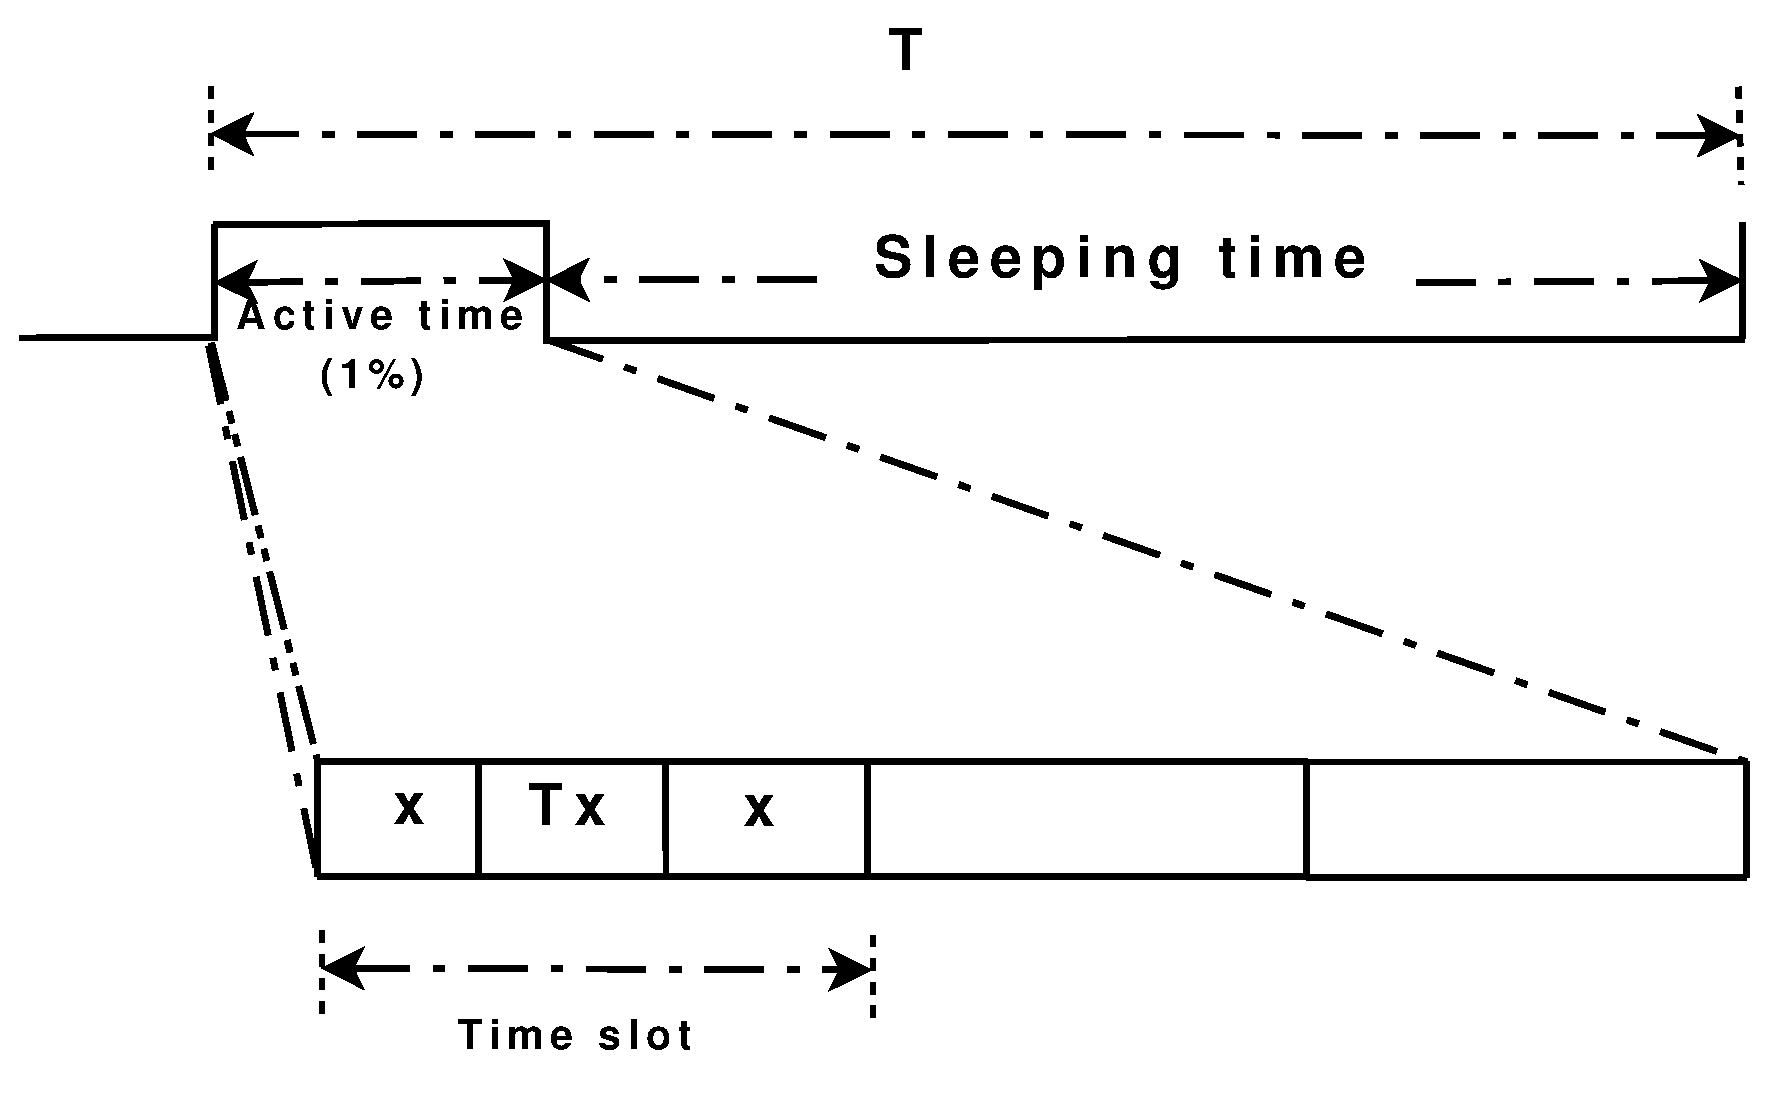
\includegraphics[width=0.5\textwidth]{guardtimesaving}
\caption{Guard time and reducing duty cycle} \label{guardtimesaving}
\end{figure}
\paragraph*{}
Let $x$ denote the guard time when the median algorithm is implemented (Figure $\ref{guardtimesaving}$). Thus, the slot
duration will be
\begin{equation}
T_{slot}=2x + T_x ,
\label{slot}
\end{equation}
where $T_x$ is the transmit time of the node.
\paragraph*{}
With $N$ slots, the duty cycle is then
\begin{equation}
D = \dfrac{NT_{slot}}{T}, \label{duty}
\end{equation}
where $T$ is the period of a time frame. \paragraph*{} Substituting ($\ref{slot}$) in ($\ref{duty}$) equation, the duty cycle becomes
\begin{equation}
D= \dfrac{N(2x+T_{slot}}{T}.
\end{equation}
With the better performance achievement with the other algorithms, the guard time can be reduced depending on the precision of the
algorithm. Let $\epsilon$ be the guard time reduction in clock cycles. Hence, the new guard time will be $2(x-\epsilon)$.
\paragraph*{} The new duty cycle becomes
\begin{equation}
D_n=\dfrac{(2(x-\epsilon)+T_x)N}{T}.
\end{equation}
Arranging the equation results in
\begin{equation}
D_n= \dfrac{(2x+T_x)N}{T} - \dfrac{(2\epsilon)N}{T}.
\end{equation}
Hence, with a performance increase in $\epsilon$ clk results in the duty cycle reduction of
\begin{equation}
D - D_n = \dfrac{(2\epsilon)N}{T}.
\end{equation}
The decrease in the guard time of the slot is thus dependent on the algorithm's performance ($\epsilon$) and the number of slots in the frame. As the number of slots increases with a constant performance increase $\epsilon$, the energy conservation also increases linearly.
\chapter{\textbf{Results and discussion}}
\section{\textbf{Simulation setup}}
%The simulation setup which is used in the research to test the performance of the presented frame synchronization algorithms is explained in this section. The simulated WSN operates in the 2.4GHz ISM band at a data rate of 2Mbps. We use a Discrete Event Simulator (DES) for the simulation. A DES\nomenclature{DES}{Discrete Event Simulator} will break down a simulation into discrete chunks. Every event will occur at some countable time moment and will be given in chronological order. The advantage is two-fold. First, simulations will not be dependant on some real-time clock, which reduces the inaccuracies fed into the simulation. Second, events can be isolated to perform certain measurements.
%\paragraph*{}
%One such DES is called OMNeT++$\cite{omnet}$. It provides a component architecture for models. Components are programmed in C++, then assembled into larger components and models using a high-level language. These components are merged into a joined simulation environment: MiXiM$\footnote{MiXiM (MIXed sIMulator) is a simulation framework for wireless and mobile networks using the OMNeT++ simulation engine.It is a collaborative project  between TU Berlin, TU Delft and Universitaet Paderborn.}$. Nodes are modeled as a set of separate components stacked upon each other. Octave$\footnote{Octave is a free program for performing numerical computations which is mostly compatible with MATLAB. It is part of the GNU project.}$ is used for interpretation of the data from the network simulator.
%\paragraph*{}
%\begin{figure}
%\centering
%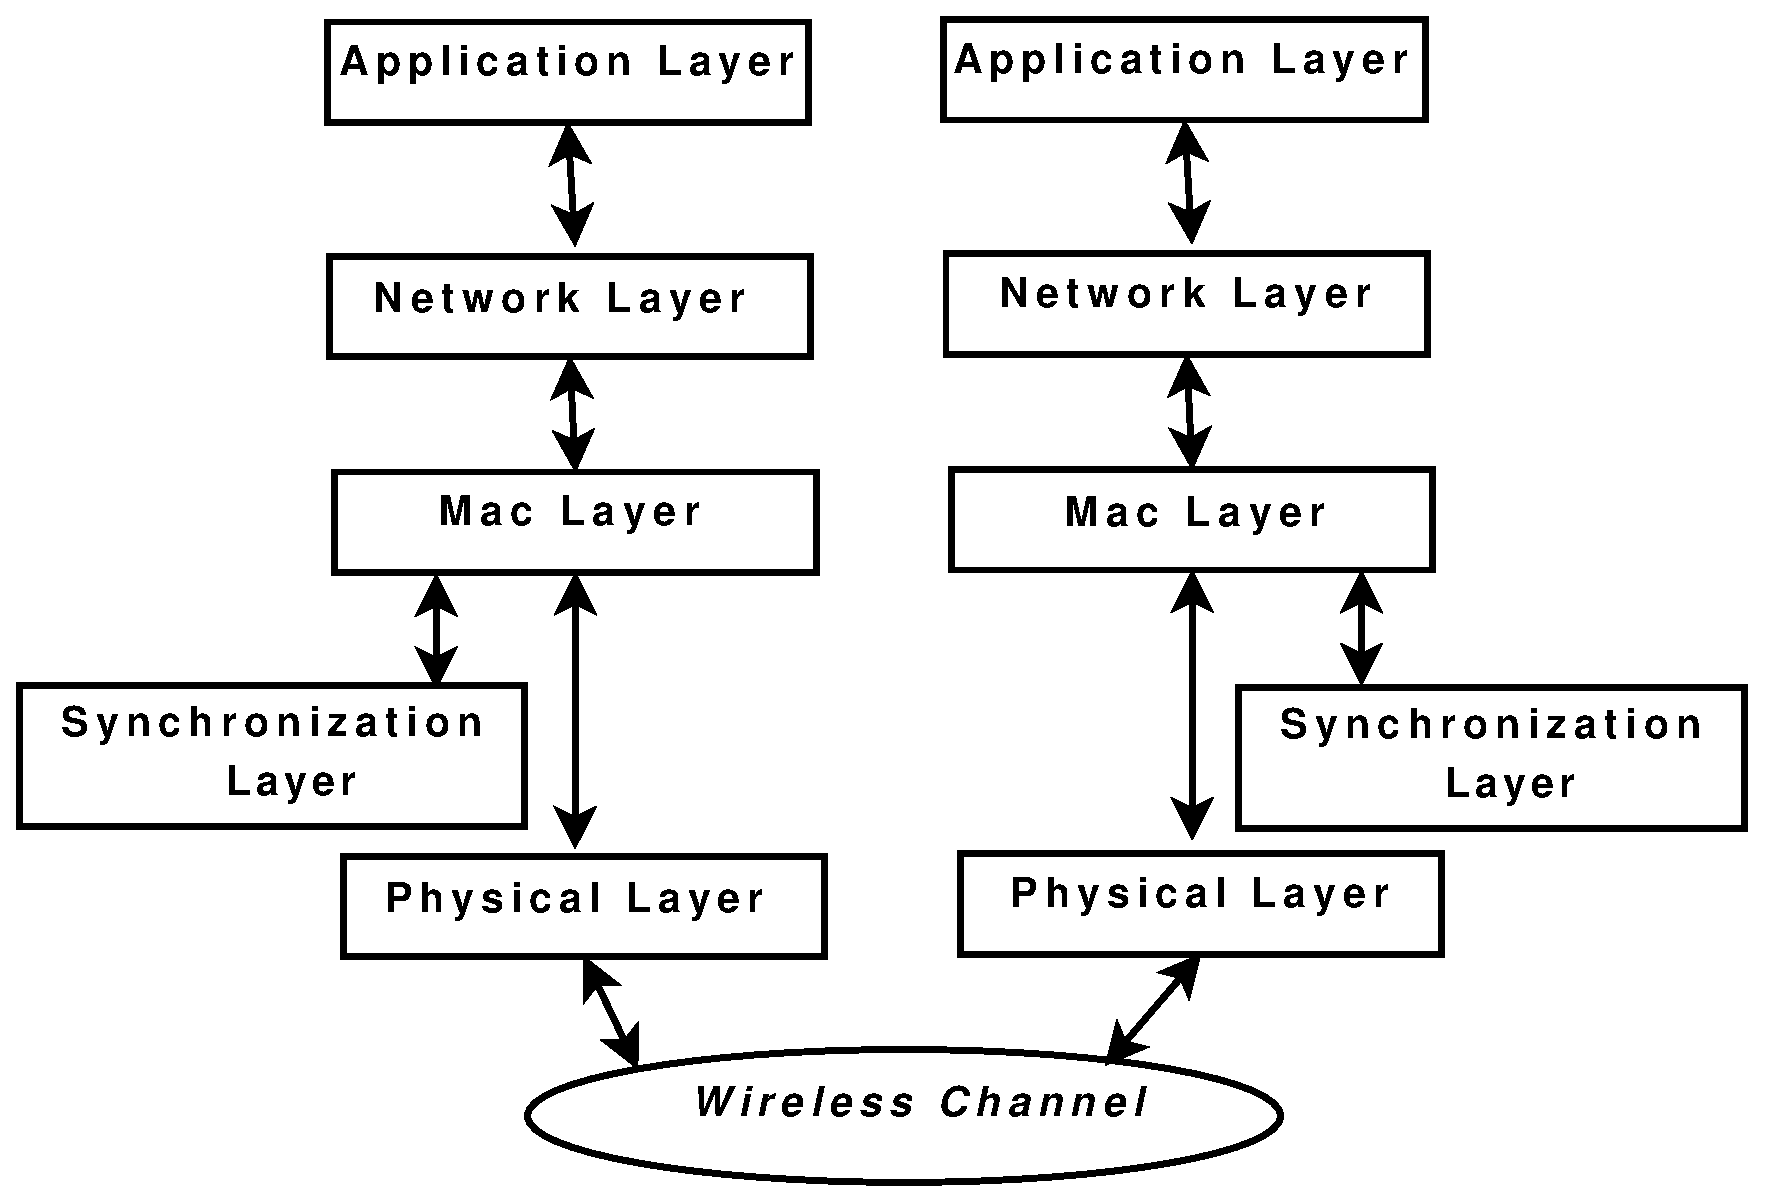
\includegraphics[width=0.5\textwidth]{osimodel}
%\caption{Abstraction model} \label{osimodel}
%\end{figure}
%As shown in Figure $\ref{osimodel}$, the synchronization is computed in a separate abstaraction layer. Each time the message is received, the time of arrival is recorded and used to calculate the next wakeup time of the node. The communication over the channels is done in a unidisc way. All nodes in range of the radio receive the data, and those that are outside are excluded. The number of nodes is varied for different scenarios. The movement of the nodes is modeled from the static to an average speed of a slowly moving object. The simulation is conducted 100 times to counter the effect of randomness introduced in the simulation.
The simulation parameters are presented in the following table.
\begin{center}
%   \caption{Simulation setup}
    \begin{tabular}{ | c | c |}
    \hline
    Duration time frame & 1s \\ \hline
    Number of slots &  10 \\ \hline
%    Attenuation constant & 2.5 \\ \hline
    Data rate &  2Mbps \\ \hline
    \end{tabular}
\end{center}
Nodes communicate by broadcasting. The start up time of the nodes is gaussian distributed random variable, $t_{io}$. The nodes are positioned uniformly across the simulation area at the start. The proposed algorithms are KF, M, WM, NLLS which represent Kalman Filter, Median, Weighted Measurments and Non Linear Least Squares respectively. A clock cycle is represented here as $clk$ which shows the resolution of the quartz crystal clock. The synchronization error is defined as the maximum difference between the wakeup time of the nodes in the neighborhood. The simulation is conducted in different scenarios and some test case results are presented here for discussion. Results with different scenarios and parameters are also included in Appendix A.
\section{\textbf{Simulation results}}
\subsubsection{\textbf{Case I}}
\begin{figure}[!h]
\centering
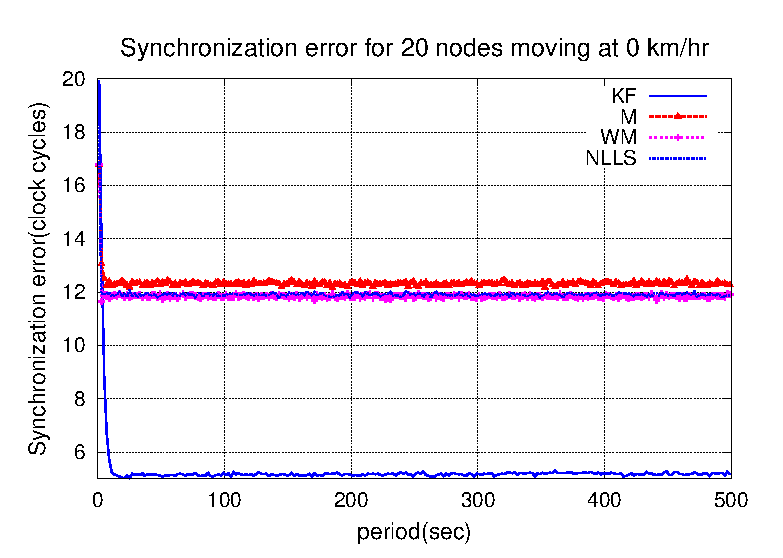
\includegraphics[width= 0.7\textwidth]{16output-s0}
\caption{Synchronization error for 20 nodes - static} \label{16output0}
\end{figure}
In the first set of simulations, the synchronization error is simulated for the nodes which are static, hence no effect of mobility. The number of nodes is taken to be $20$ and $50$ in this set of simulations.  \paragraph*{}
\begin{figure}
\centering
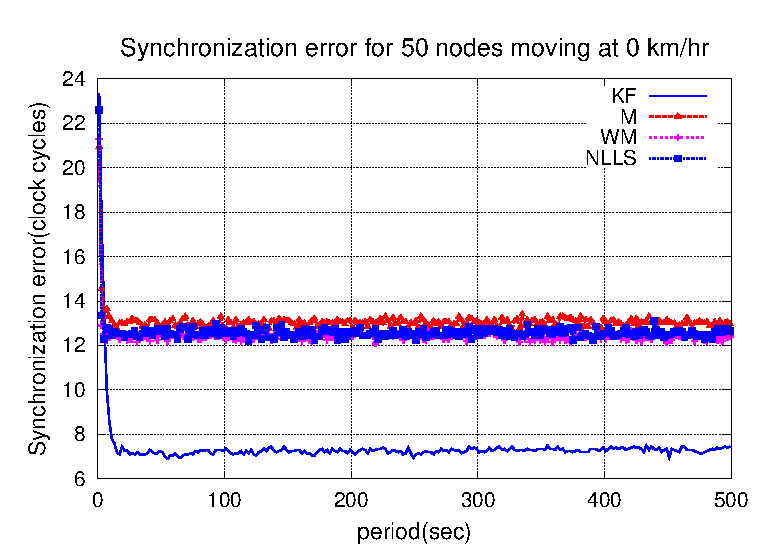
\includegraphics[width= 0.7\textwidth]{50output-s0}
\caption{Synchronization error for 50 nodes - static} \label{50output0}
\end{figure}
Figure $\ref{16output0}$ shows the synchronization error for $20$ nodes operating in a static environment. The algorithms achieve a stable synchronization. As NLLS and WM has the same effect as the Median in case of stable network, the performance of both algorithms is similar with that of Median. Without the dynamic nature of the network, both tend to equal the average of the phase errors. KF has the best performacesince correcting the phase errors involves predict and update which results in better precision. \paragraph*{}
Figure $\ref{50output0}$ is the result of a simulation for $50$ nodes. The synchronization error in general increases as the number of nodes increases. Comparing the individual algorithms, KF has a precision of $7clk$ whereas NLLS and WM have a better performance each. Median results in a lower performance on average.
\subsubsection{\textbf{Case II}}
In second set of simulations, the mobility of the nodes is taken into account. Here, the number of the nodes is taken to be $20$. The simulations are conducted for different speeds, at average speeds of $6km/hr$ and $20km/hr$. The chosen speeds emulate the speed of a walking man and an average speed of a slowly moving vehicle.
\paragraph*{}
Figure $\ref{16output6}$ shows 20 nodes with a speed which is an gaussian random variable with mean $6km/hr$ and standard
deviation of 1$km/hr$. WM and NLLS show a better tolerance to dynamic networks due to the algorthms capapbilty to synchronize towards a more stable network. NLLS has also a better tolerance with less value given for large phase errors. Hence, WM and NLLS perform
better concerning the synchronization of the frame than the Median.  Median algorithm has a disruptions which made the network out-of-synchronization, resulting in high synchronization errors at times. This occurs due to the mobility of the nodes which disrupts the stability networks as it tries to compute the median of the phase errors, as indicated in Chapter 3. KF outperforms all.
\paragraph*{}
\begin{figure}
\centering
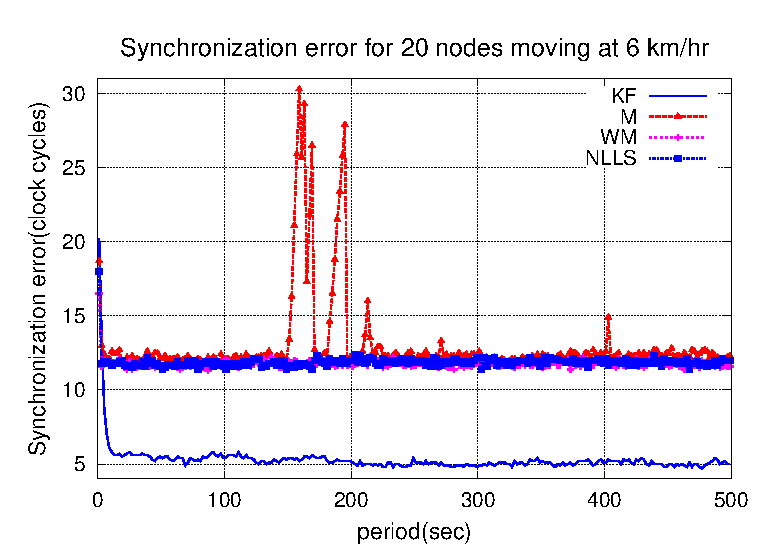
\includegraphics[width=0.7\textwidth]{16output-s6}
\caption{Synchronization error for 20 nodes - speed 6km/hr} \label{16output6}
\end{figure}
\begin{figure}
\centering
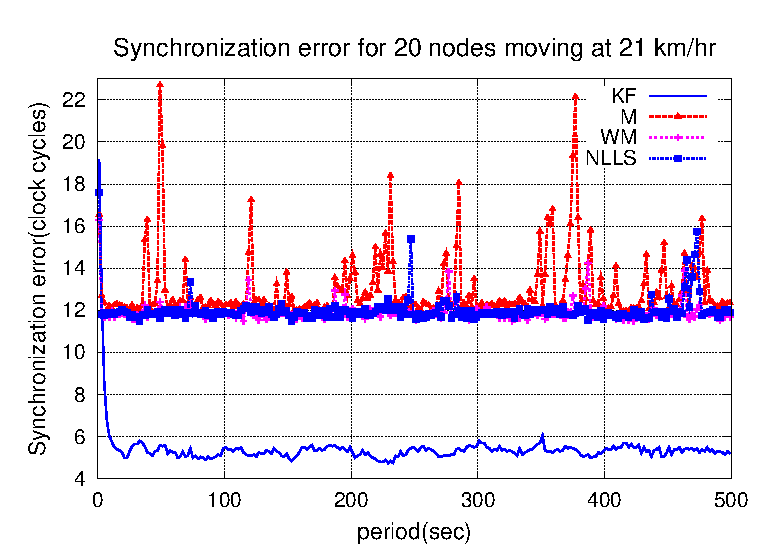
\includegraphics[width=0.7\textwidth]{16output-s20}
\caption{Synchronization error for 50 nodes - speed 20km/hr}
\label{16output20}
\end{figure}
The speed of the nodes is changed to a random variable with mean $20km/hr$ and standard deviation $1km/hr$. The simulation results are presented in Figure $\ref{16output20}$. KF performs the best showing that the algorithm is stable in dynamic networks. WM and NLLS perform good when it comes to stability. As the dynamics of the networks increases, Median becomes more unstable and exhibits large synchronization error. NLLS and WM have a stable performance when the network becomes dynamic with constantly changing connection between the nodes.
\paragraph*{}
The relative comparison of the algorithms performance improvement with the Median is shown in Figure $\ref{16output-error}$ for nodes moving at $20km/hr$. WM and NLLS perform, on average, $6-8\%$ better than Median, but with more tolerance in handling the disruptions. The best performer, KF, has on average $60\%$ better performance than the Median one.
\begin{figure}
\centering
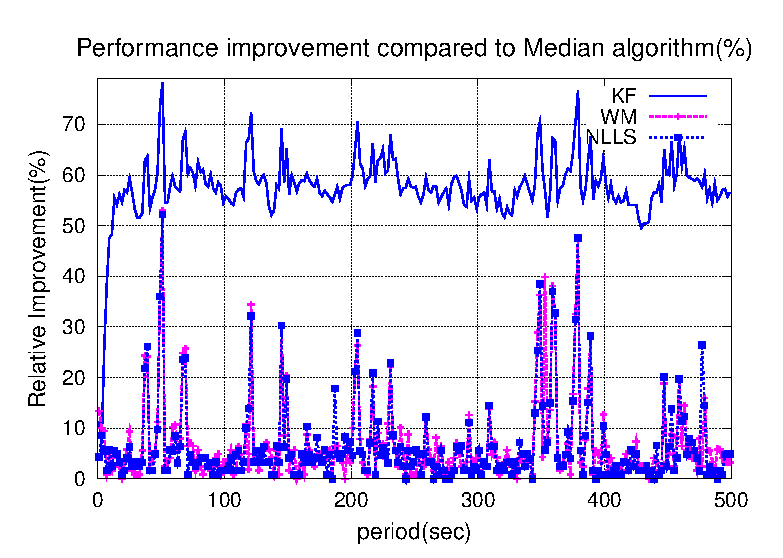
\includegraphics[width= 0.7 \textwidth]{16output-error}
\caption{Relative performance improvement of algorithms from Median - 20 nodes} \label{16output-error}
\end{figure}
\subsubsection{\textbf{Case III}}
In this set of simulations, the number of the nodes is increased, to $50$. With slowly moving nodes ($6km/hr$), the results are shown in Figure $\ref{50output6}$. Large disruptions occur when using Median due to nodes moving slowly in the surrounding (leave the network and join again after some time), resulting in a larger drift with neighbors before getting back to the network. NLLS and WM perform better when it comes to stability, as out-of-sync nodes are forced to join the stable network. KF has the best preformance, both in precision and stability. On average, KF has $7clk$ as a synchronization error.
\paragraph*{}
\begin{figure}
\centering
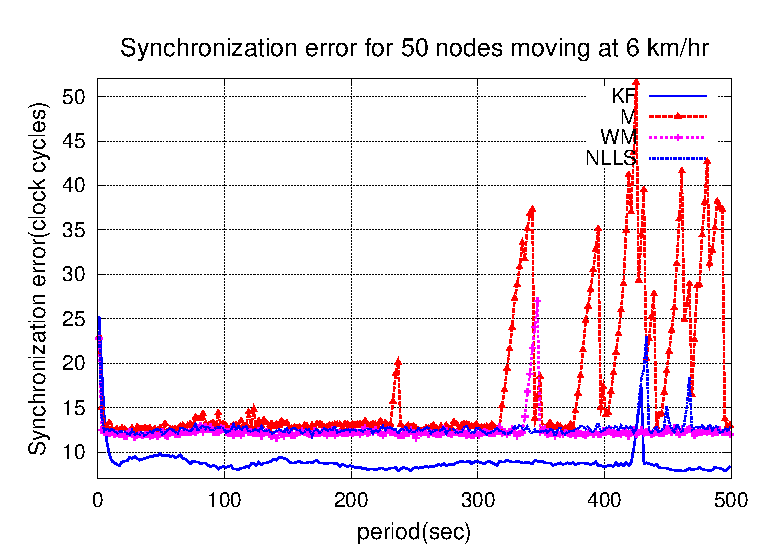
\includegraphics[width=0.7\textwidth]{50output-s6}
\caption{Synchronization error for 50 nodes - speed 6km/hr}
\label{50output6}
\end{figure}
\begin{figure}
\centering
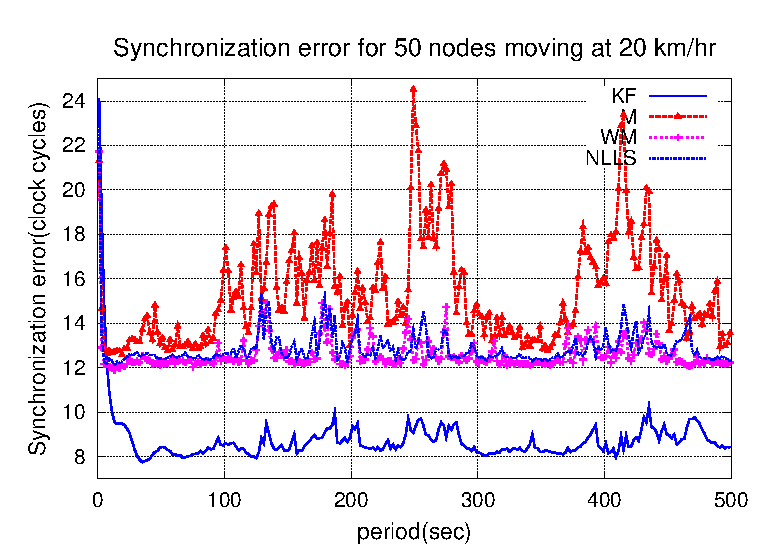
\includegraphics[width=0.7\textwidth]{50output-s20}
\caption{Synchronization error for 50 nodes - speed 20km/hr} \label{50output20}
\end{figure}
With a speed of $20km/hr$, the simulation results are presented in Figure $\ref{50output20}$. As the speed increases, the instability
on the synchronization of the nodes also increases, which makes the Median more prone to high synchronization errors. WM has better
tolerance towards mobility of the nodes, whereas the NLLS does well regarding stability. KF has the best precision, at $9clk$. As the
speed increases, the precision of the synchronization increases too since faster speed results in faster synchronization within the network.
\paragraph*{}
For the set of nodes with a higher speed , a relative comparison is made to see the performance of the nodes with the Median algorithm. The Median algorithm is shown to perform the worst in this case. There are a lot of disruptions in the network, making it more unstable whereas the other algorithms adapt to the changes faster. Figure $\ref{50output-error}$ shows that KF performs the best against Median algorithm, $45\%$. WM and NLLS perform well against Median too, $20\%$ on average. It has been shown that the median is prone to error in case of high dynamics in the network.
\begin{figure}[!h]
\centering
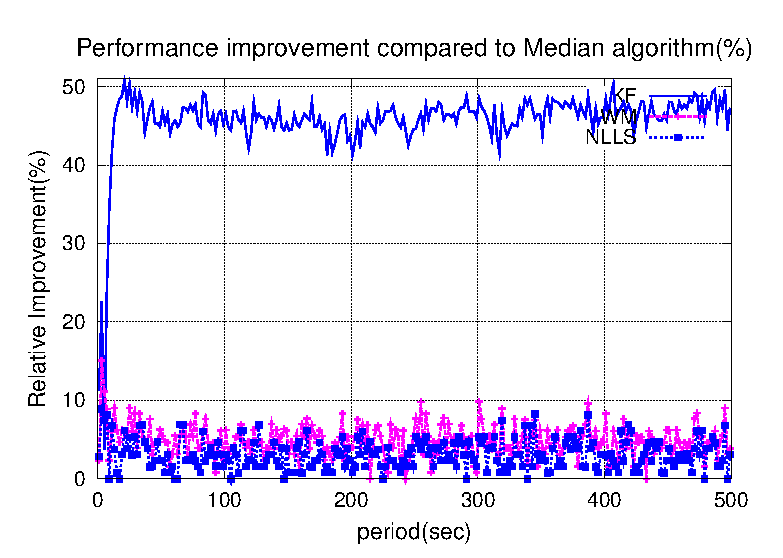
\includegraphics[width=0.7  \textwidth]{50output-error}
\caption{Relative performance improvement of algorithms from Median - 50 nodes} \label{50output-error}
\end{figure}
\paragraph*{}
Simulation is conducted using the different parameters and the results are presented in the Appendix A.
\section{\textbf{Energy consumption}}
%\begin{figure}
%\centering
%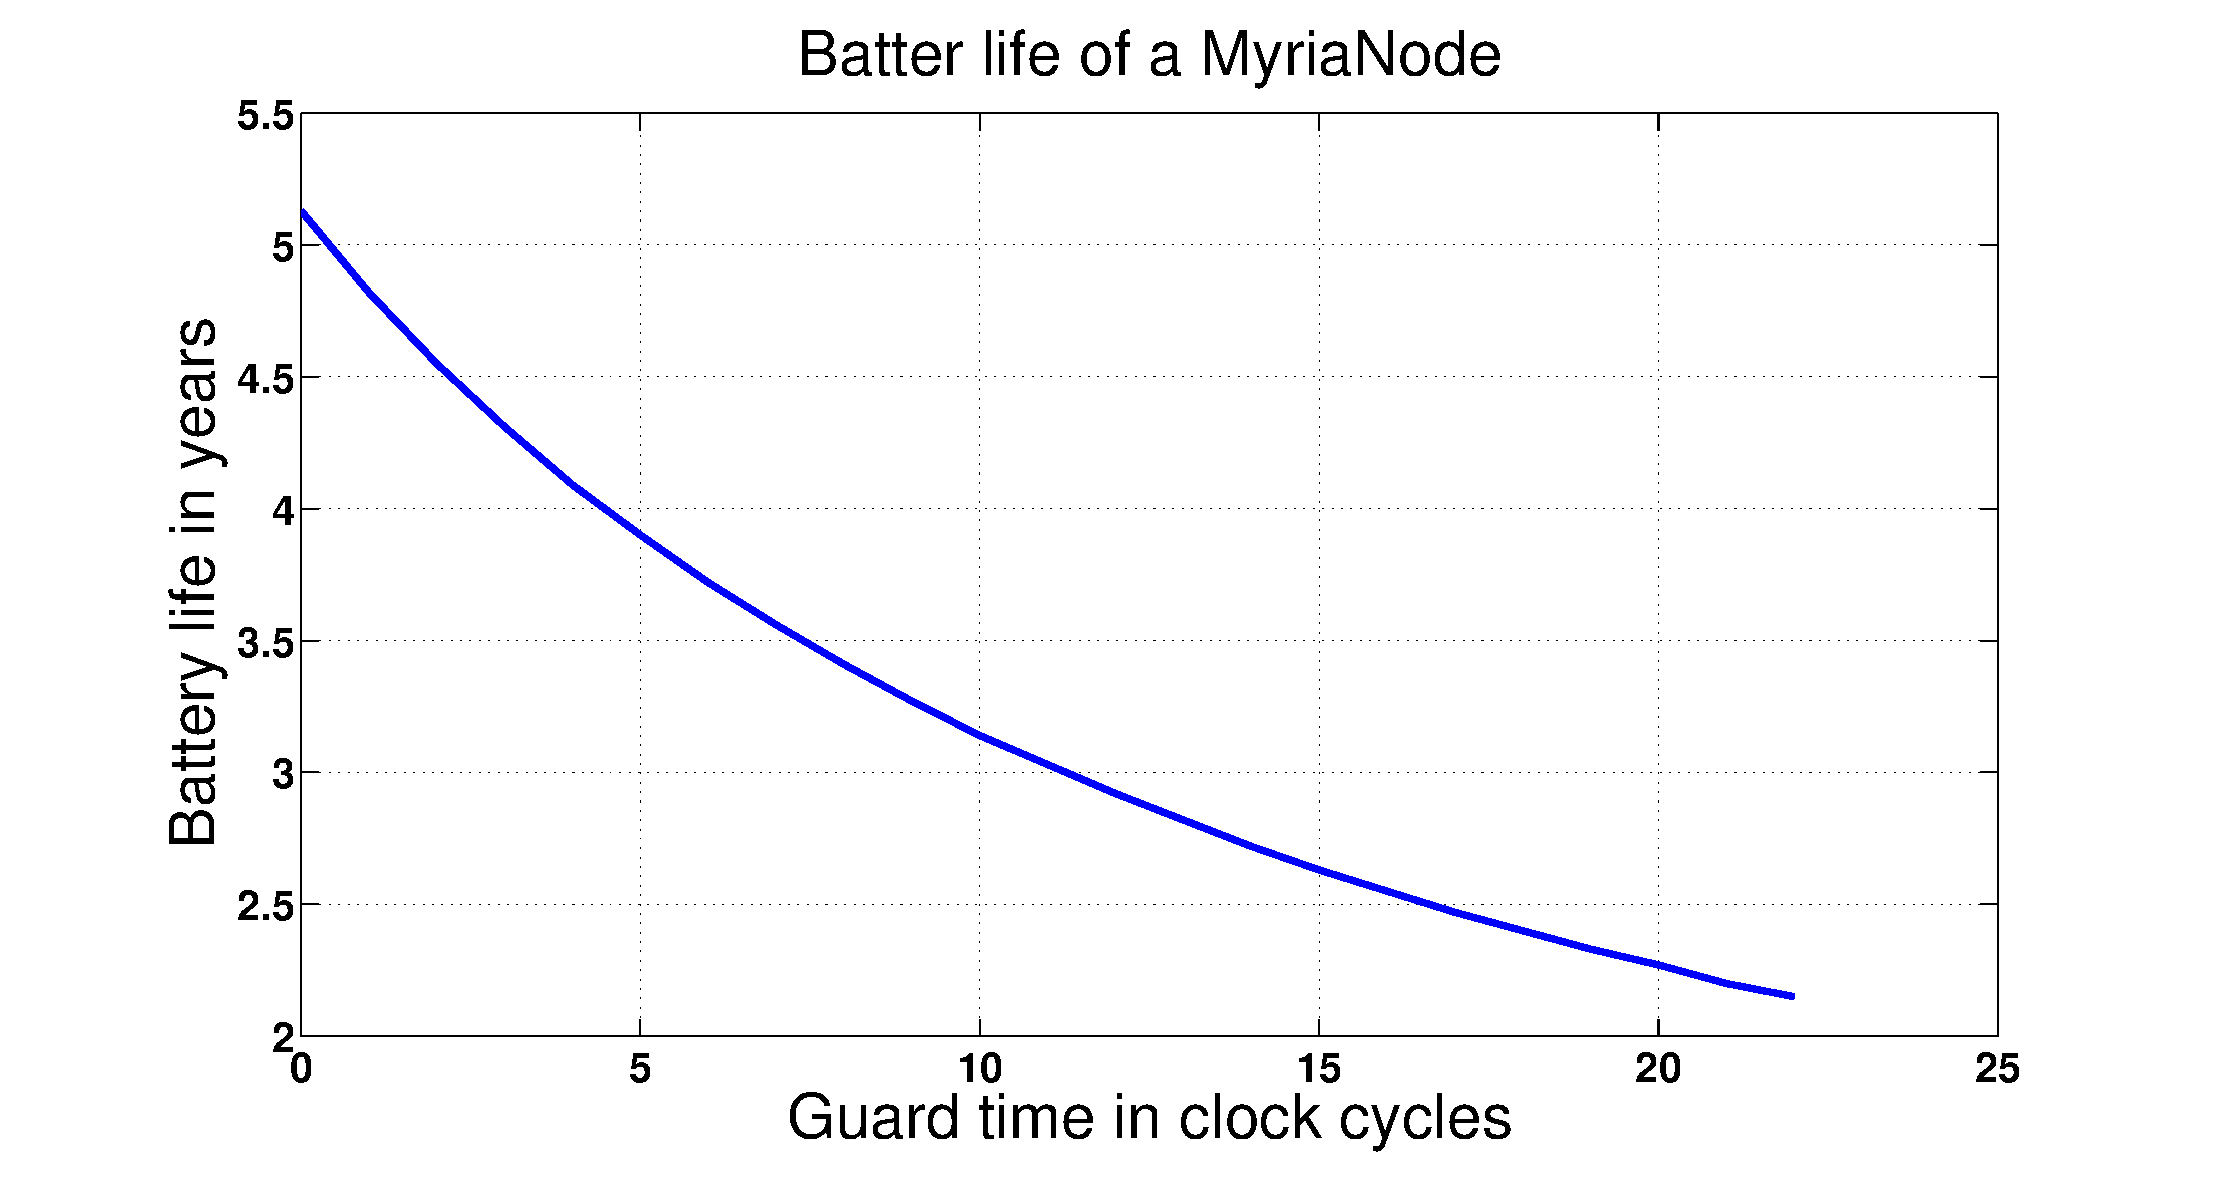
\includegraphics[width=0.7\textwidth]{guardsave}
%\caption{The energy consumption of guard time per RX slot}
%\label{guardsave}
%\end{figure}
%As the results in the previous section shows, KF algorithm performs well in all conditions, so do WM and NLLS when stability is a vital metric. The downside in implementing these algorithms, despite the performance gain that all have against the Median is the energy consumption. As the algorithms are going to be implemented on the sensor nodes, the energy consumption is a priority in the study of embedded system algorithm development in WSN. The algorithms are written in C and implemented on the test nodes to see the effect that they are going to have on the energy consumption of the nodes.
%\begin{center}
%    \begin{tabular}{ |p{2cm} | p{4.75cm} |}
%    \hline
%    Algorithm & Average Execution Time \\ \hline
%    M &  65 $\mu$s \\ \hline
%    NLLS & 82.5 $\mu$s \\ \hline
%    WM &   90 $\mu$s \\ \hline
%    KF &  195 $\mu$s  \\ \hline
%    \end{tabular}
%\label{tab}
%\end{center}
%The table $\ref{tab}$ shows the average execution time of the algorithms implemented on the test MyriaNode. This doesn't show the
%exact energy consumption of the algorithms but it can give us an approximation on the relative comparison of the algorithms about the energy consumption on the MyriaNode. It can be mapped to the energy consumption of the algorithms.
%%As the table shows, the consumption of WM is 5$\%$ higher than the median algorithms. This is also true for NLLS and KF which consume 9$\%$ and 4 $\%$ higher than the median algorithm respectively.
%\paragraph*{}
%In order to reduce the energy that is going to be spent on the algorithm with a better performance, the guard time of the slot can be reduced, due to a better performance showing by KF, WM and NLLS. The energy consumption of the guard time is shown in Figure
%$\ref{guardsave}$. The length of the guard time has a close-to-linear relation with the power being consumed in listening to the channel.
%Thus, with the performance gain obtained, the guard time of the slot can be decreased, hereby decreasing the energy consumption of the node in general. This energy save is in a per slot basis. As the number of slots increases, the energy to be saved increases.
%\paragraph*{}
%Communcation costs around 5 times more than computing, as per the measured data from Chess shows. So, by reducing the communication time and increase the computing cost of the node, a net gain in energy can be obtained.
\textbf{Additional energy expenditure}\par \noindent
As the results in the previous subsection shows, KF algorithm performs well in all conditions, so do WM and NLLS when stability is a vital metric. The downside in implementing these algorithms, despite the performance gain achieved, is the energy consumption. As the algorithms are going to be implemented on the sensor nodes, the energy consumption is a priority in embedded system algorithm development. The algorithms are written in C and implemented on the test nodes to see the effect that they are going to have on the energy consumption of the nodes and presented below.\newline
The results shown in Table $\ref{tab1}$do not reflect the exact energy consumption of the algorithms as the energy consumption is dependent on other factors besides the execution time. But it can be used to put the comparison into perspective.
\begin{table}[!h]
    \caption{Table to represent the energy expenditure of the algorithms}
    \begin{tabular}{ |c | p{3.5cm} | p{3.5cm} |c | }
    \hline
    Algorithm & Average Execution Time per frame & Increase in execution time per frame & Energy Consumed per frame \\ \hline \hline
    M &  65 $\mu$s & 0 & 0  \\ \hline
    NLLS & 82.5 $\mu$s & 7.5$\mu$s & 63 $pJ$  \\ \hline
    WM &   90 $\mu$s & 25$\mu$s & 210 $pJ$ \\ \hline
    KF &  150 $\mu$s  & 85$\mu$s &  714 $pJ$\\ \hline
    \end{tabular}
\label{tab1}
\end{table}
\newline
\textbf{Energy gain}\par \noindent
%As communication costs more than computation[datsheet MyriaNode v2.0], a tradeoff can be done.
In order to reduce the energy that is going to be spent on the algorithm with a better performance, the guard time of the slot can be reduced, due to a better performance showing by KF, WM and NLLS.
Hence, $t_{guard}$ for KF is taken to be 10$clk$ whereas the guard time for WM and NLLS is taken to be $24clk$ each from the simulation results. $t_{guard}$ for the Median is taken to be 26$clk$. The number of slots is taken to be 10, so the total guard time per frame will be 10 times $t_{guard}$. In the following table, the energy saving is calculated in comparison with the Median.
\begin{table}
        \caption{Table to show the energy saving due to the guard time reduction}
    \begin{tabular}{ |c | c |c | c |  }
    \hline
    Algorithm & Guard time per frame & Reduction in $t_{guard}$ per frame & Energy saving per frame\\ \hline \hline
    M &  792 $\mu$s x 10 & 0 & 0 \\ \hline
    NLLS & 732 $\mu$s x 10 & 600 $\mu$s & 16.27$\mu J$\\ \hline
    WM &   732 $\mu$s x 10 & 600 $\mu$s & 16.27$\mu J$ \\ \hline
    KF &  305 $\mu$s x 10 & 4870 $\mu$s & 132.07$\mu J$\\ \hline
    \end{tabular}
\label{tab2}
\end{table}
The length of the guard time has a close-to-linear relation with the power being consumed in listening to the channel. Thus, with the performance gain obtained, the guard time of the slot can be decreased, hereby decreasing the energy consumption of the node in general. Comparing the energy consumption and the energy expenditures, a large net gain can be obtained from the proposed algorithms. It can be noted here that communication costs more than computation (as listening radio consumes more energy than CPU active time). Since the length of the guard time is dependent on the number of slots, the energy to be saved increases as the number of slots increases.\newline
The comparison on energy gain and expenditure is shown in Figure $\ref{guardsave1}$. As the number of slots increases, the net gain in energy increases.
\begin{figure}[!h]
\centering
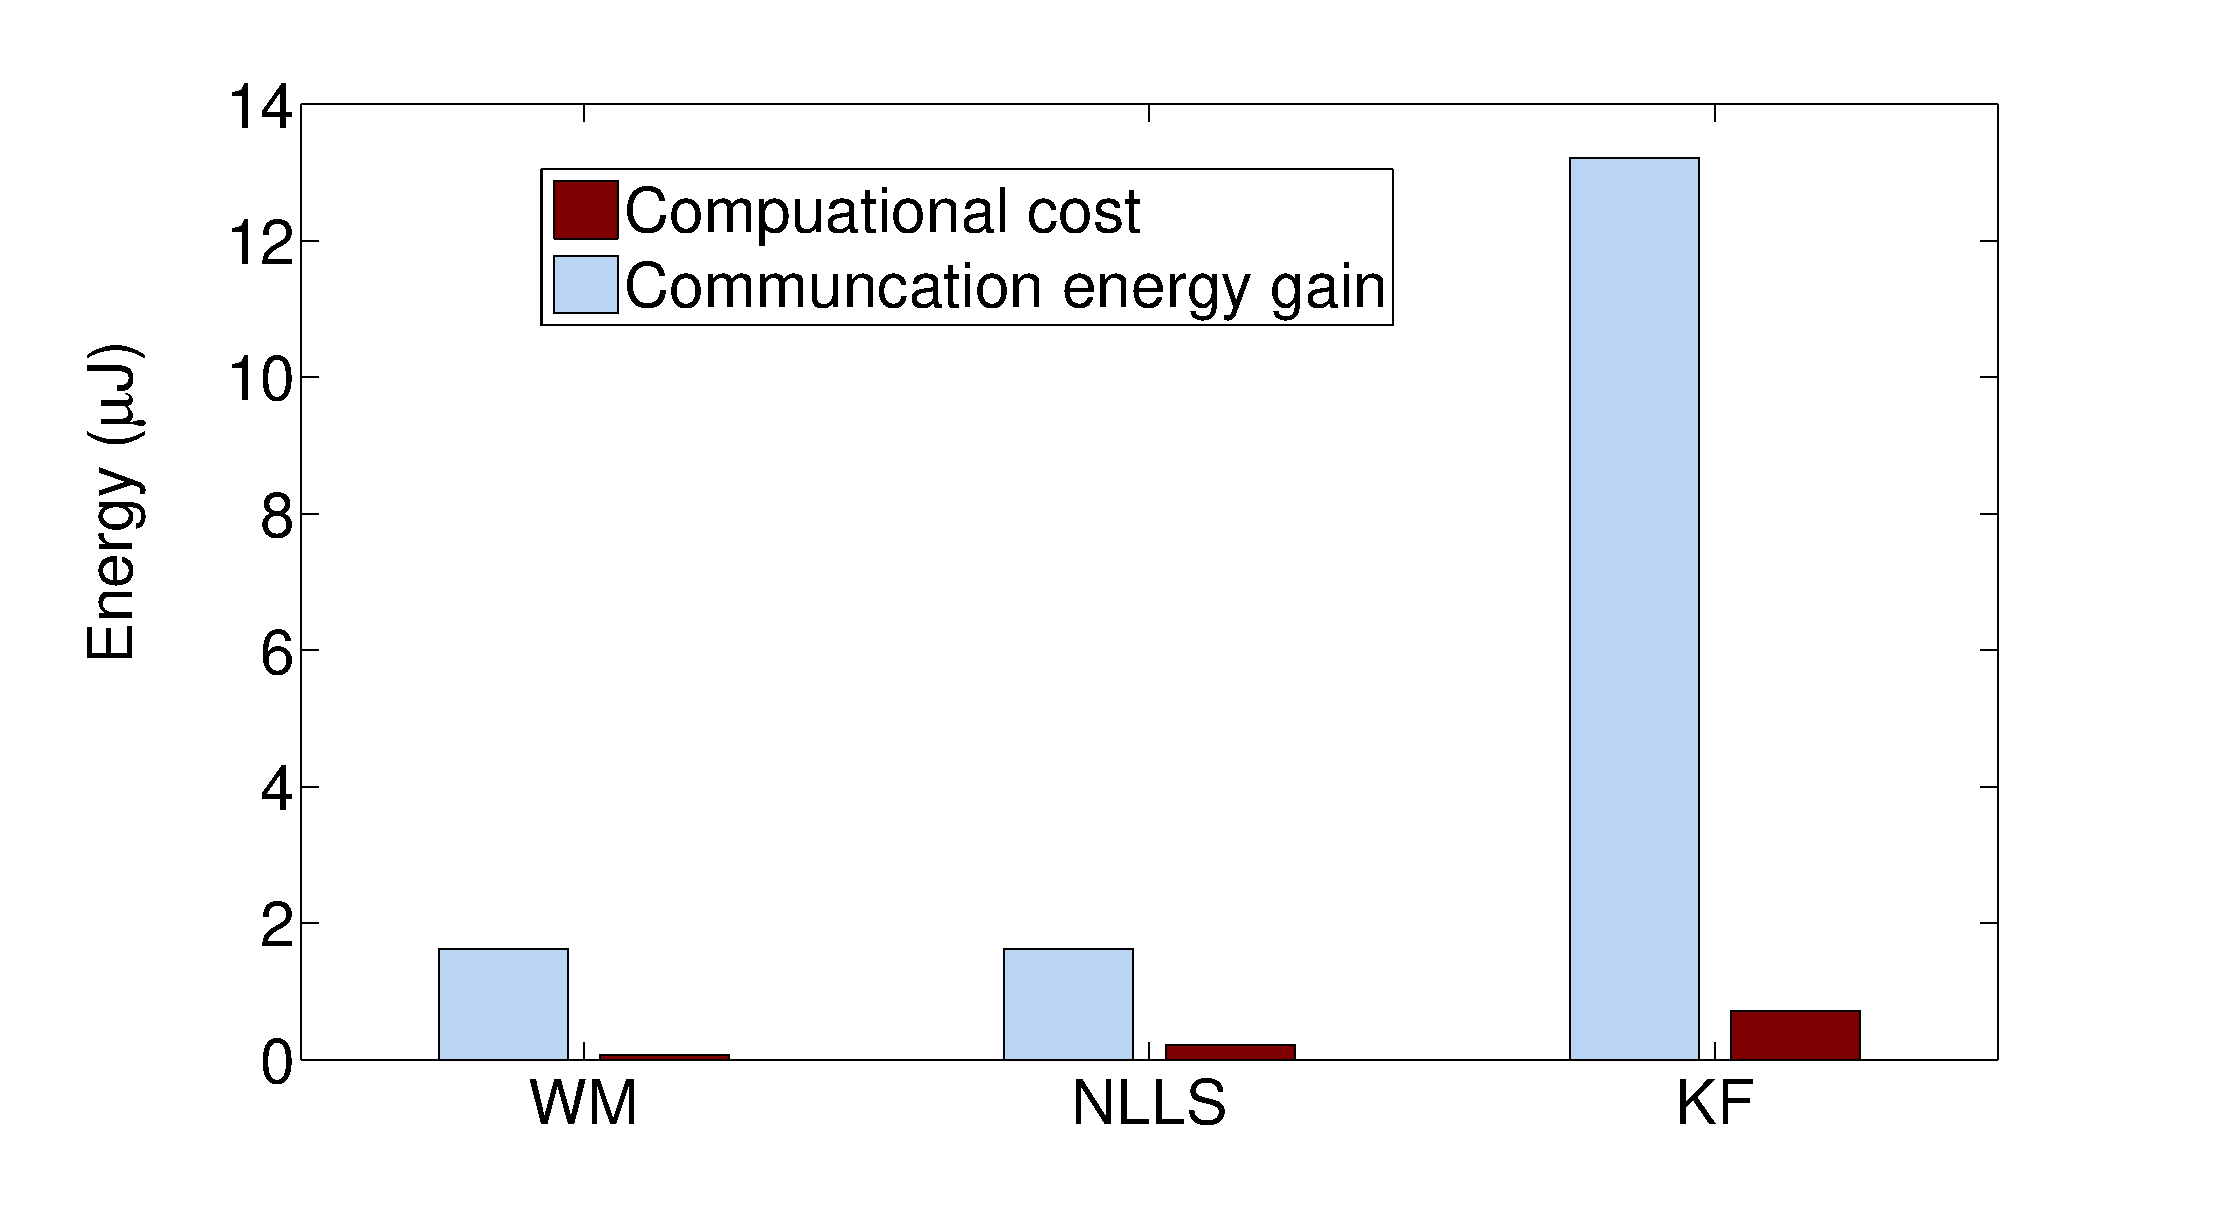
\includegraphics[width=0.7\textwidth]{commvscompute}
\caption{The energy gain of reducing the guard time compared with the compuational cost per RX slot}
\label{guardsave1}
\end{figure}
\chapter{\textbf{Conclusion and recommendation}}
\section{\textbf{Conclusion}}
Decentralized synchronization algorithms are proposed for a TDMA-based WSN using Weighted Measurements (WM), Non Linear Least Squares(NLLS) and Kalman Filter (KF) methods. Simulation is conducted with different scenarios, especially taking the effect of mobility. Comparison of the algorithms with the currently implemented Median algorithm is conducted and the results are presented.
\paragraph*{}
In a static environment where the nodes are stationary, the KF performs the best whereas the WM and NLLS have shown a similar performance since they incline to calculate the average of the phase errors. In terms of stability, all the three algorithms have shown a similar performance.
\paragraph*{}
WM and NLLS show a very good tolerance in a dynamic network. Having a
faster adaptation to the changes in the network made the algorithms
preferred ones to a network characterized with dynamic behavior. Besides, simple designs of the algorithms is an advantege in energy-constrained WSN. KF estimation of the next wakeup time is yields a very good performance with its recursive and dynamic nature. KF has also good stability making it resistant to topology changes occurring in the network.
\paragraph*{}
Using these algorithms for a TDMA-based WSN synchronization (WM, NLLS and KF), the precision of the synchronization error as well as the stability increases. This in turn has a positive impact on the energy consumption of the nodes because the synchronization period, $T_{sync}$ can be increased or the guard time of the node's frame, $t_{guard}$, can be reduced to achieve the same performance as the Median algorithm. Results are presented and discussed. But in the downside, the energy consumption of the algorithms is greater than the Median algorithm's energy consumption as the algorithms are more complex computationally. Analysis is made and presented about the energy saving made by decreasing the guard time of the slot. A net gain of battery life can thus be achieved by using the proposed algorithms.
\section{\textbf{Recommendation}}
\paragraph*{}
As is the case with new design techniques for any system of protocol, there is always room for improvement. Although the performance of all our approaches are more precise and stable,  some factors which could be considered to make it a good synchronization scheme on all aspects have been identified. Below are some suggestions on the future work.
\begin{itemize}
\item
Different software power minimization techniques can be applied to reduce the power consumption of the algorithm implementation, making them more energy efficient for implementation.
\item  As the main sources of error for the clock inaccuracies are identified, resolving these errors is one approach which can be cost effective as well as simple in implementation. This can be achieved using the available resources like the temperature sensor in the microcontroller of the MyriaNode. Constantly updating the temprature of the surrounding and correcting the drift on the node can achieve a better precision on the synchronization.
\item
Practical implementation of the algorithms and inspect the behavior is another step in pefecting the algorithms. Upon the completion of the ongoing project on developing a Software Defined Radio (SDR) for the inspection of the nodes' wakeup times, a proper evaluation and enhancements on the algorithms, being implemented on the MyriaNodes, is achievable. Real time feedbacks can be used to improve the algorithms towards perfection.
\end{itemize}
\appendix
%\chapter{\textbf{Lower bound of synchronization}}
%As in distributed synchronization, a network of nodes equipped with hardware clocks with bounded drift is considered
%here. Nodes compute logical clock values based on their hardware clocks and information that they have, and the goal is to
%synchronize the nodes' logical clocks as closely as possible, while satisfying certain validity conditions.
%%\begin{figure}[!h]
%%\centering
%%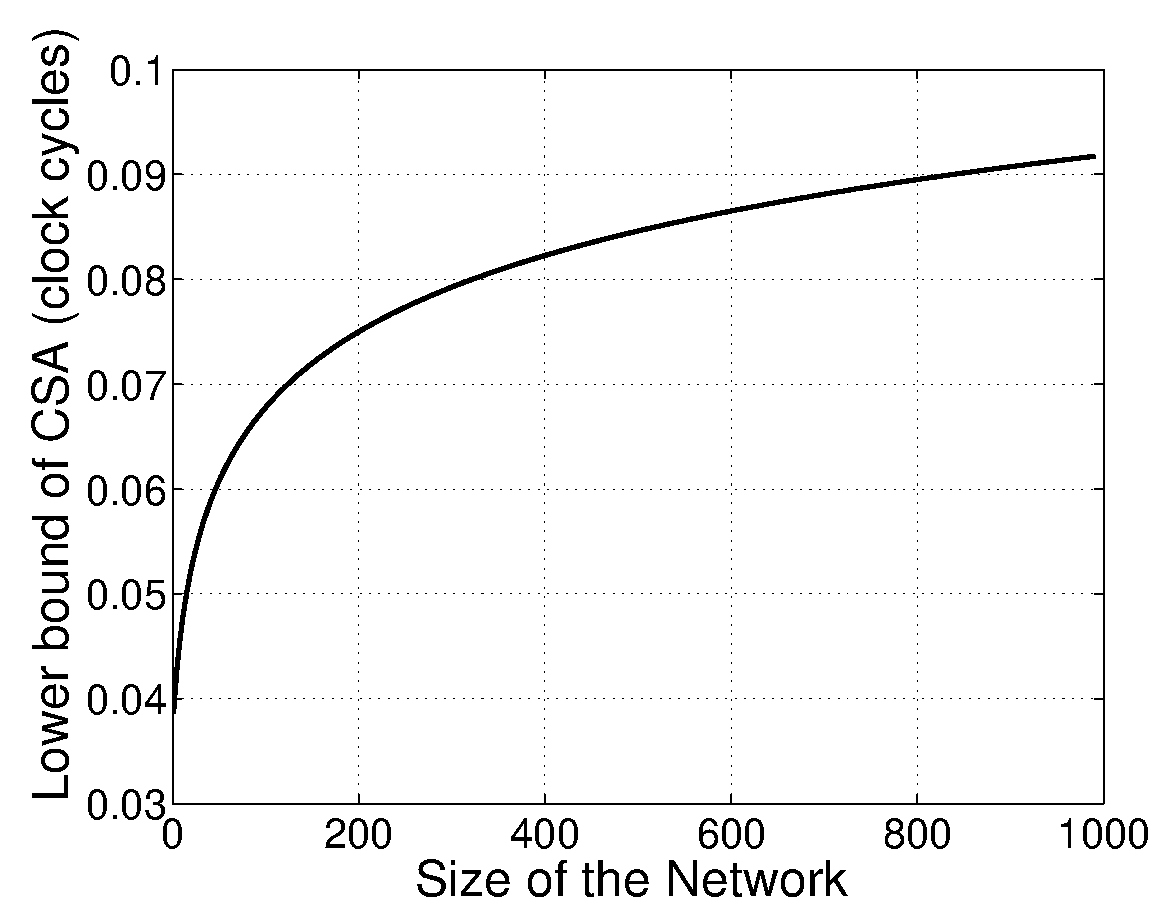
\includegraphics[width=0.5 \textwidth]{lowerbound}
%%\caption{Network size and the lower bound of synchronization}
%%\label{gradient}
%%\end{figure}
%\paragraph*{}
%There are different approaches towards the lower bound that a synchronization algorithm achieve. In $\cite{gradient}$, the clock drift is taken to be zero and the delay impact on the lower bound of the synchronization algorithm is presented. But a more realistic approach is presented in $\cite{gradient2}$. Gradient clock synchronization is shown to require that the skew between any two nodes' logical clocks be
%bounded by a nondecreasing function of the uncertainty in message delay (call this the distance) between the two nodes. Nearby nodes
%are required to be closely synchronized, and allow far away nodes to be more loosely synchronized. Hence, the result is that the worst
%case clock skew between two nodes at distance $d$ from each other is
%\begin{equation}
%\Delta L \geq \dfrac{\tilde \rho d}{8(1+\tilde \rho)}\dfrac{log(n-1)}{log(\dfrac{8(1+\tilde \rho)}{\tilde \rho}log(n-1))}.
%\end{equation}
%where $n$ is the number of nodes in the network. This means that synchronization is not only a local property, in the sense that the clock skew between two nodes depends not only on the distance between the nodes, but also on the size of the network. \paragraph*{}
%Our lower bound implies, as in the case of MyriaNed, that the TDMA protocol with a fixed slot granularity will fail as the network grows, even if the maximum degree of each node stays constant. As the network size grows, the lower bound of the synchronization also increases.
\chapter{Simulation results}
%\section{\textbf{Median as a synchronization method}}
%The performance of Median algorithm is dependent on the gain factor used in the offset calculation. Figure $\ref{gainfactor}$ shows the performance of the Median algorithm for different gain factors, and the optimum value of the gain factor is chosen for the comparison of Median algorithm with the proposed algorithms for synchronization.
%\begin{figure}[!h]
%\centering
%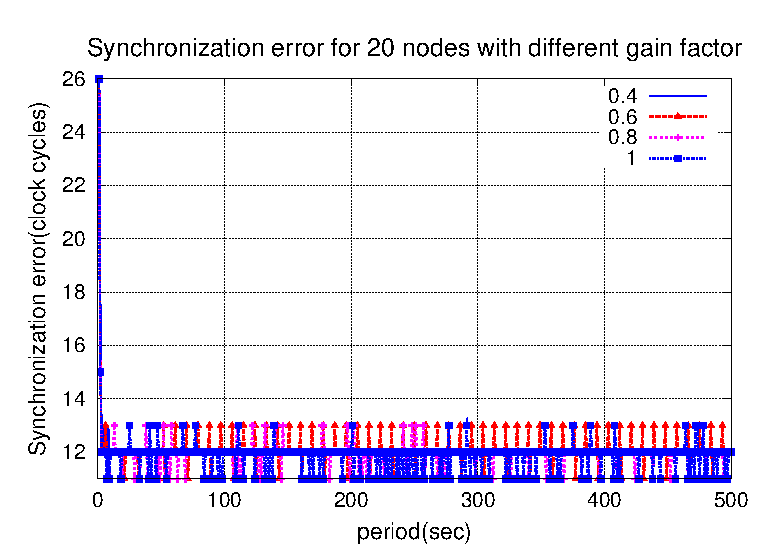
\includegraphics[width= 0.7 \textwidth]{gainfactor}
%\caption{Median algorithm with different gain factors} \label{gainfactor}
%\end{figure}
\section{\textbf{Synchronization frequency}}
Increasing the time interval in which a synchronization algorithm is executed has the advantage in
 energy conservation. On the other hand, the performance of the network decrease as the nodes are
 getting sycnrhoniazed less frequently. Simulation results of different scenrarios are conducted to see the effect of the synchronizatio frequency and are presented here.
\paragraph*{}
Simulation is conducted for different synchronization frequencies $T_{sync}$ on the KF algorithm. Figure $\ref{tsync0}$ shows the performance of KF with varying the synchronization frequency $T_{sync}$ for static nodes. As the synchronization frequency increases, the performance of the algorithm decreases, herby increasing the synchronization error. Even if this approach decreases the computational cost on the nodes, it has a negative impact by decreasing the network performance.
\begin{figure}[!h]
\centering
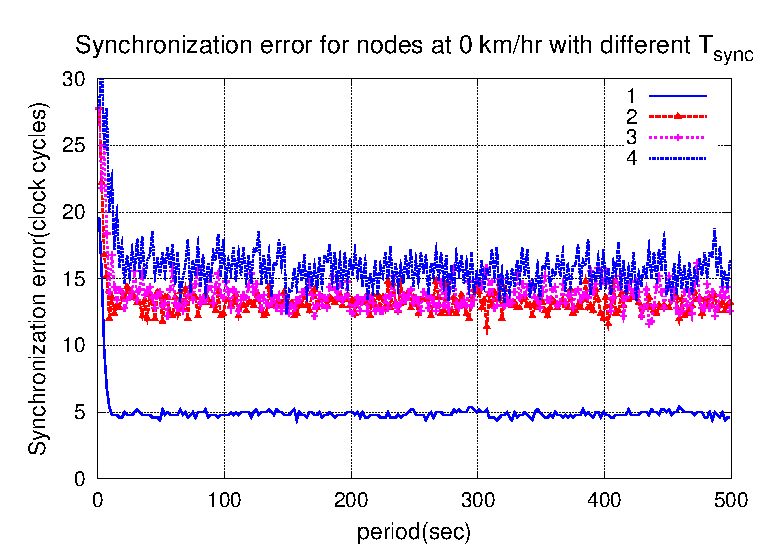
\includegraphics[width= 0.7\textwidth]{tsync0}
\caption{Synchronization error of a KF for static nodes with different $T_{sync}$} \label{tsync0}
\end{figure}
In this set of simulations, the speed of the nodes increased to see the effect of mobility on the
 synchronization frequency. Figure $\ref{tsync6}$ and Figure $\ref{tsync20}$ shows the performance of KF at different speeds, 6$km/hr$ and 20$km/hr$ respectively.
As the speed increases, the synchronization error increases. Besides the synchronization error,
 the ability of KF to adapt to changes is also affected due to the increased in the synchronization frequency. As shown in the results, there are large disruptions in the synchronization error when the nodes speed is set to an average speed of $6km/hr$. With the increased speed, the synchronization error decreases as the nodes are fast in joining the network that they left.
\begin{figure}[!h]
\centering
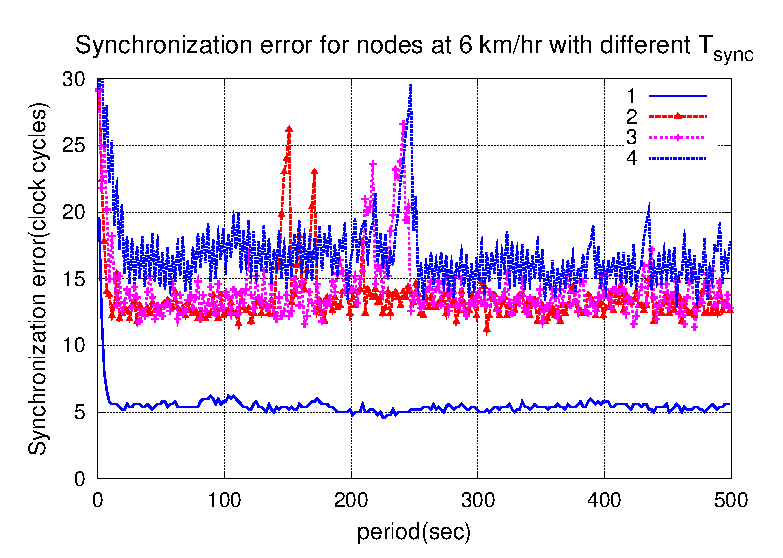
\includegraphics[width= 0.7\textwidth]{tsync6}
\caption{Synchronization error of a KF for nodes at 6$km/hr$ with different $T_{sync}$} \label{tsync6}
\end{figure}
\begin{figure}[!h]
\centering
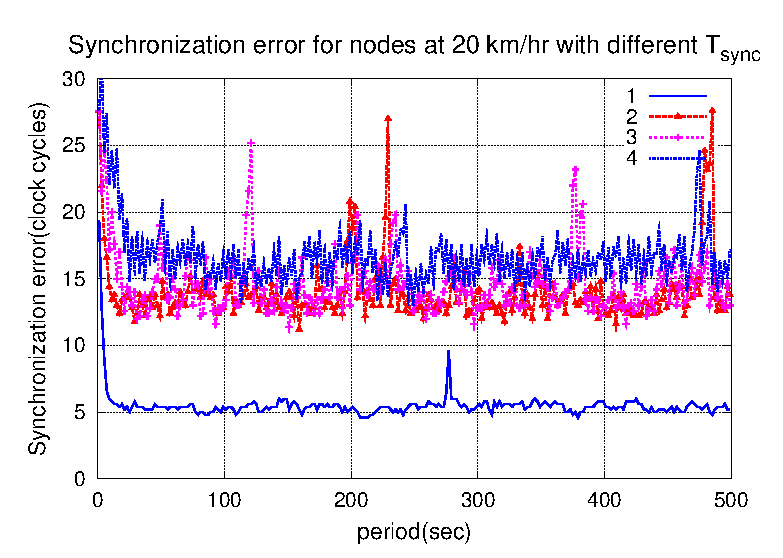
\includegraphics[width= 0.7 \textwidth]{tsync20}
\caption{Synchronization error of a KF for nodes at 20$km/hr$ with different $T_{sync}$} \label{tsync20}
\end{figure}
As the speed of the nodes increases to $20km/hr$, the effect of increasing $T_{sync}$ also increases with diversions of synchronization error. As the faster moving nodes join the network in less time, the upper bound of the synchronization error is less as the speeds increases.
\section{\textbf{Synchronization error for nodes with different speeds}}
As in a real world scenario, a simulation is conducted with nodes having different speeds. The speed of the nodes is taken to be a gaussion distributed random variable with a mean speed of $10km/hr$ and standard deviation of $5km/hr$.
\paragraph*{}
The synchronization error for nodes travelling with different speeds is given in Figure $\ref{varspeed16}$ for 20 nodes. Similar results are obtained for the networks where unstability is observed in the Median algorithm. WM and NLLS has a good tolerance towards the dynamic nature of the network. KF has the best precision, in addition to the stabililty.
\begin{figure}[!h]
 \centering
 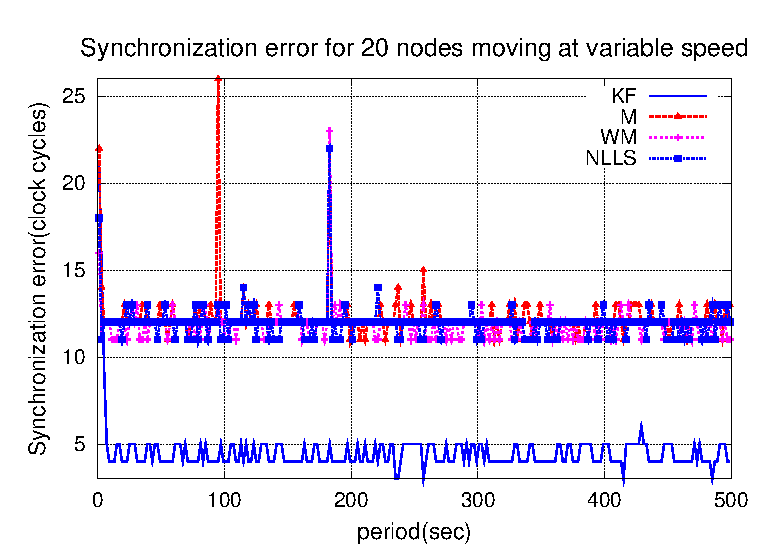
\includegraphics[width=0.7\textwidth]{varspeed20}
 \caption{Synchronization error for 20 nodes moving at different speeds}
 \label{varspeed16}
\end{figure}
\paragraph*{}
For 50 nodes, the simulation result for is shown in Figure $\ref{varspeed50}$.In both cases, KF performs the best out of all the algorithms whereas the tolerance of WM is better than Median. NLLS also performs better than Median interms of stablity.
\begin{figure}[!h]
 \centering
 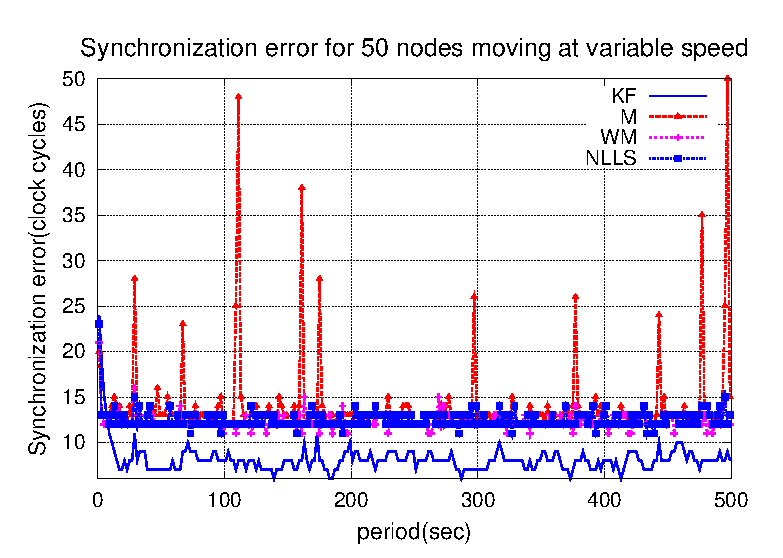
\includegraphics[width=0.7\textwidth]{varspeed50}
 \caption{Synchronization error for 50 nodes moving at different speeds}
 \label{varspeed50}
\end{figure}
\section{\textbf{The effect of number of nodes on KF}}
The synchronization error increases as the number of nodes increases, as dictated by the gradient equations in $\cite{gradient}$ and $\cite{gradient2}$. Figure $\ref{diffno}$ shows the synchronization error for KF using different number of nodes, distributed across the simulation area uniformly. The synchronization error increases besides the fact that the logical distance (timewise) between two nodes remain the same.
\begin{figure}[!h]
\centering
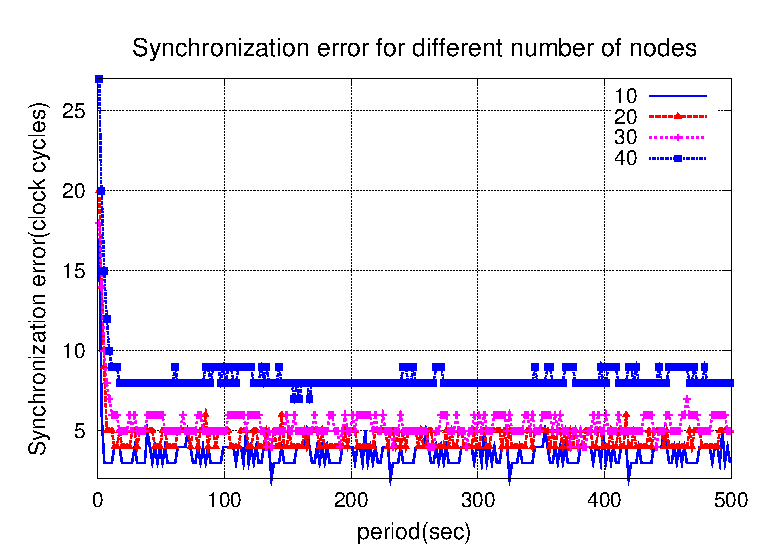
\includegraphics[width= 0.7 \textwidth]{diffno}
\caption{Synchronization error of KF for different number of static nodes}
\label{diffno}
\end{figure}
\section{\textbf{Battery life of a Myrianode versus the guard time}}
Using a 2400 mAh battery, the battery life of a MyriaNode is calculated by varying the length of the guard time. Figure $\ref{batterylife}$ shows how the battery life is affected by the increae in the guard time of the nodes frame. The model uses a TDMA frame of 10 slots.
\begin{figure}[!h]
\centering
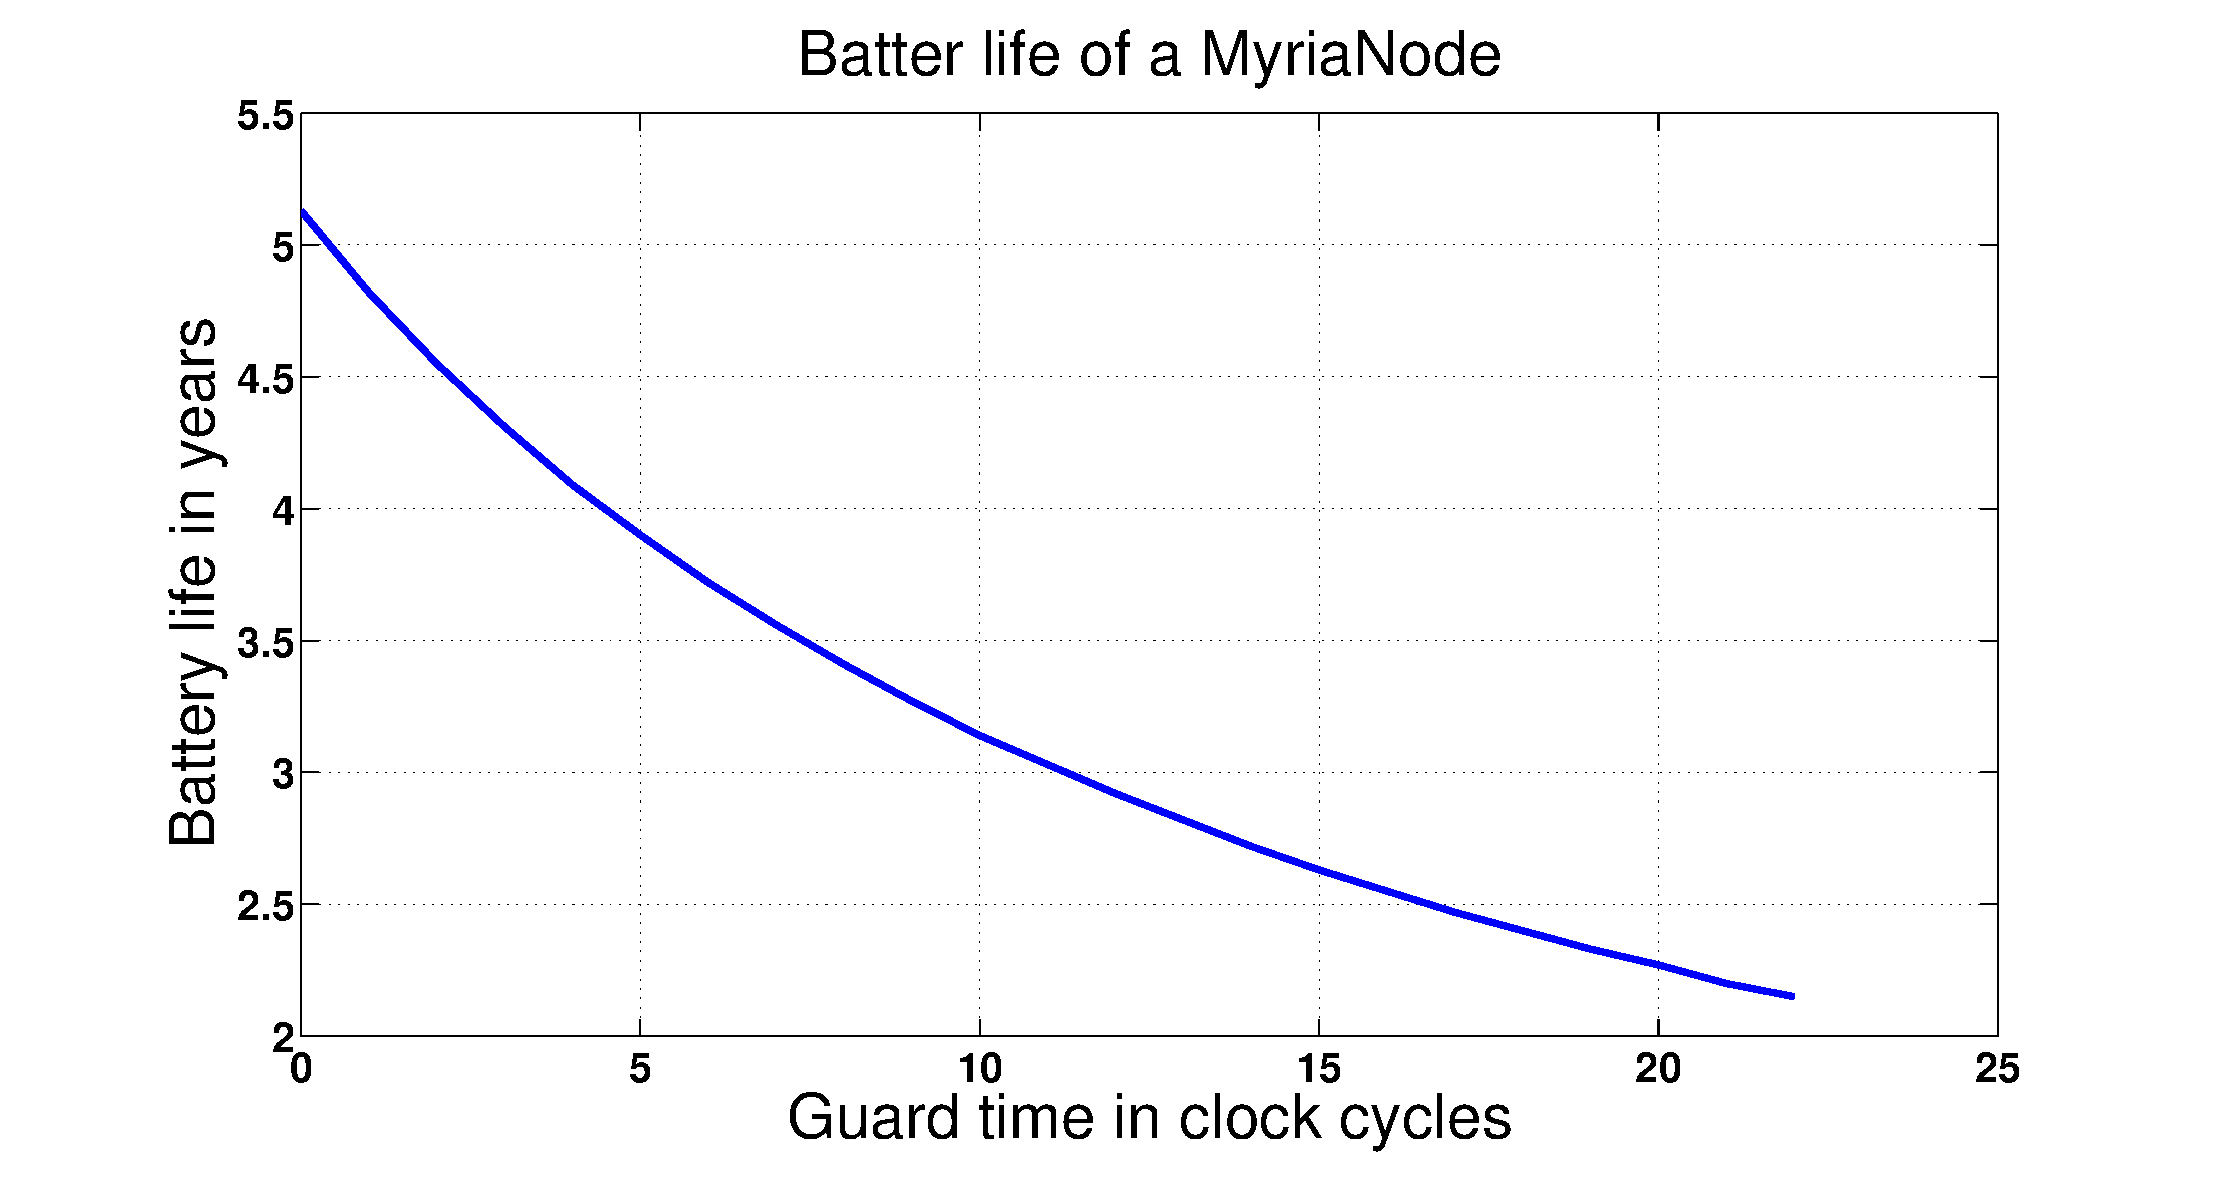
\includegraphics[width = 0.7\textwidth]{guardsave}
\caption{Battery life of a Myrianode vs the guard time}
\label{batterylife}
\end{figure}
\chapter{MyriaNode}
\begin{wrapfigure}{r}{0.4\textwidth}
  \begin{center}
    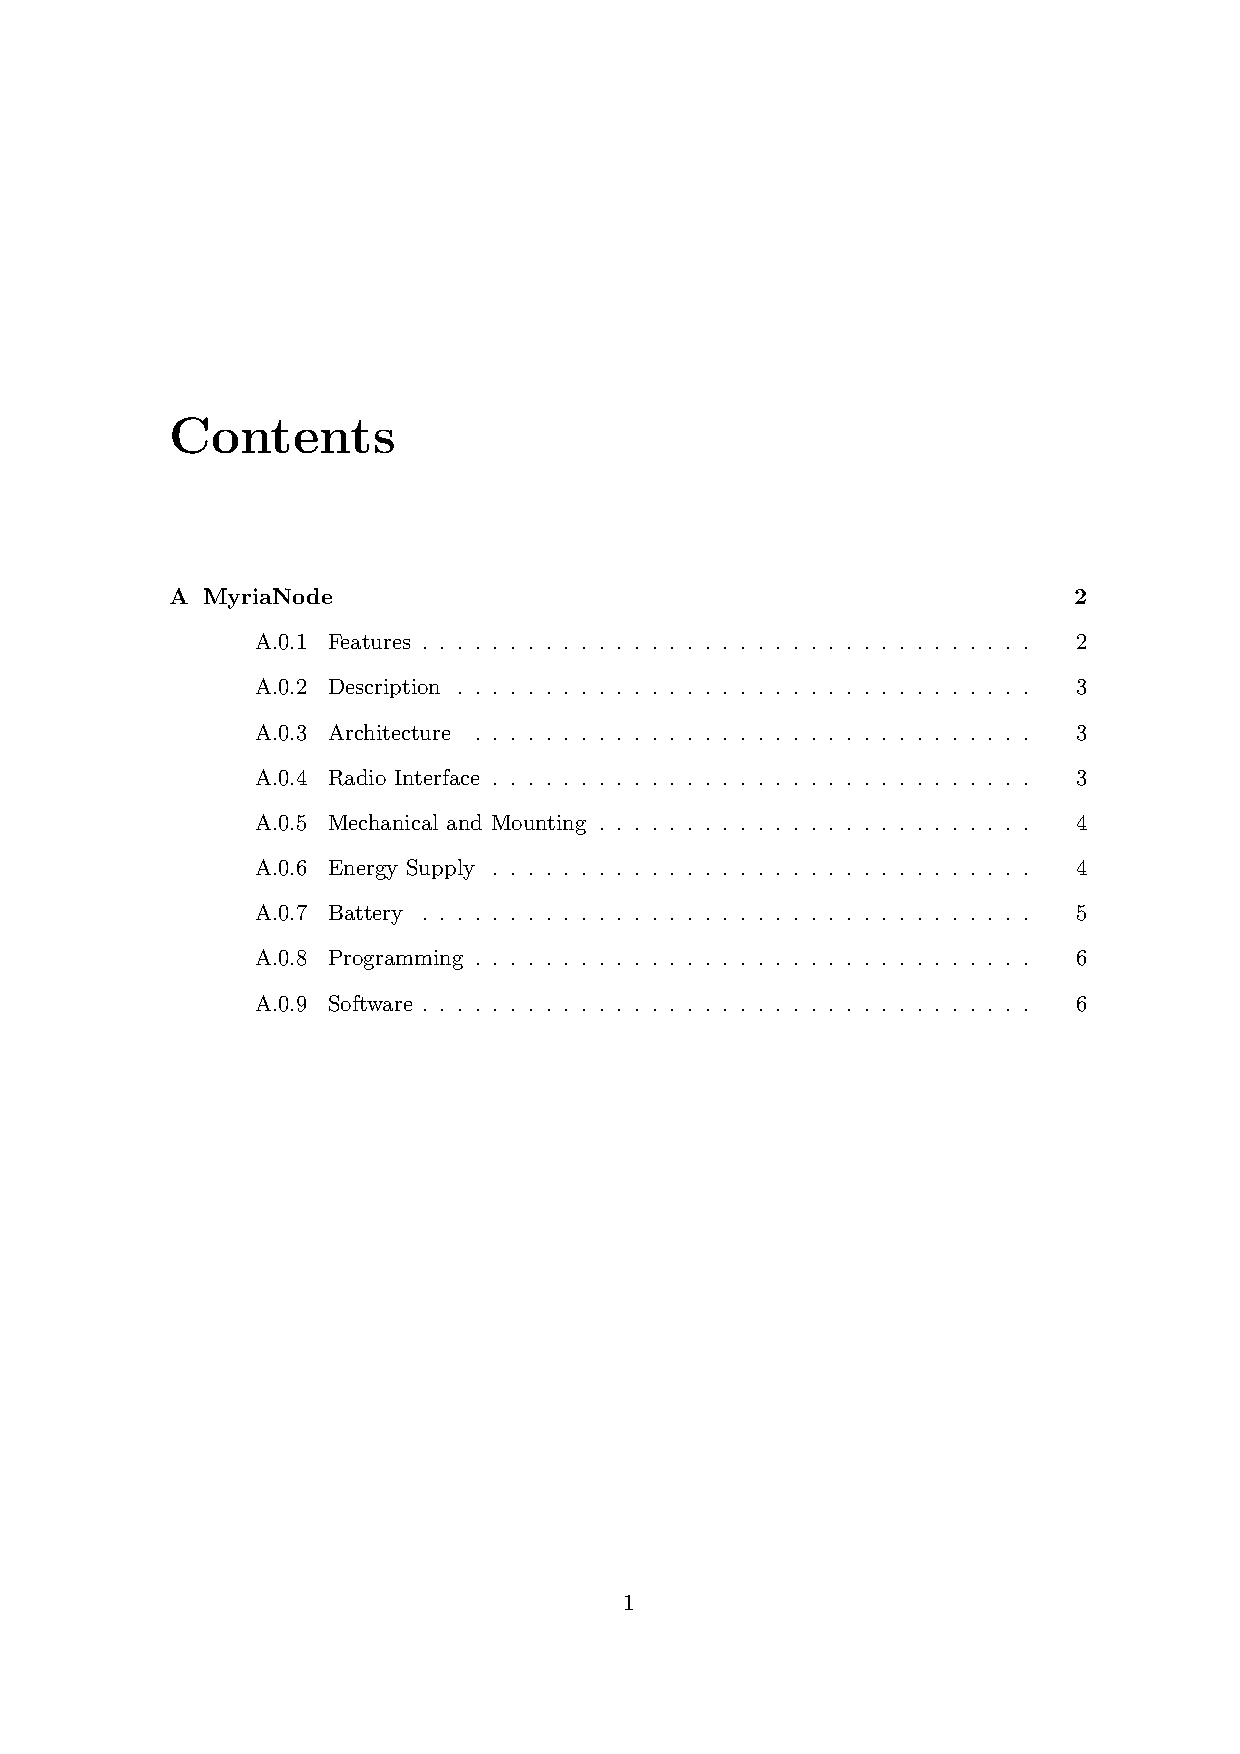
\includegraphics[width=0.38\textwidth]{myrianode}
  \end{center}
  \caption{MyriaNode v2.0}
\end{wrapfigure}
%\begin{figure}[!h]  \centering 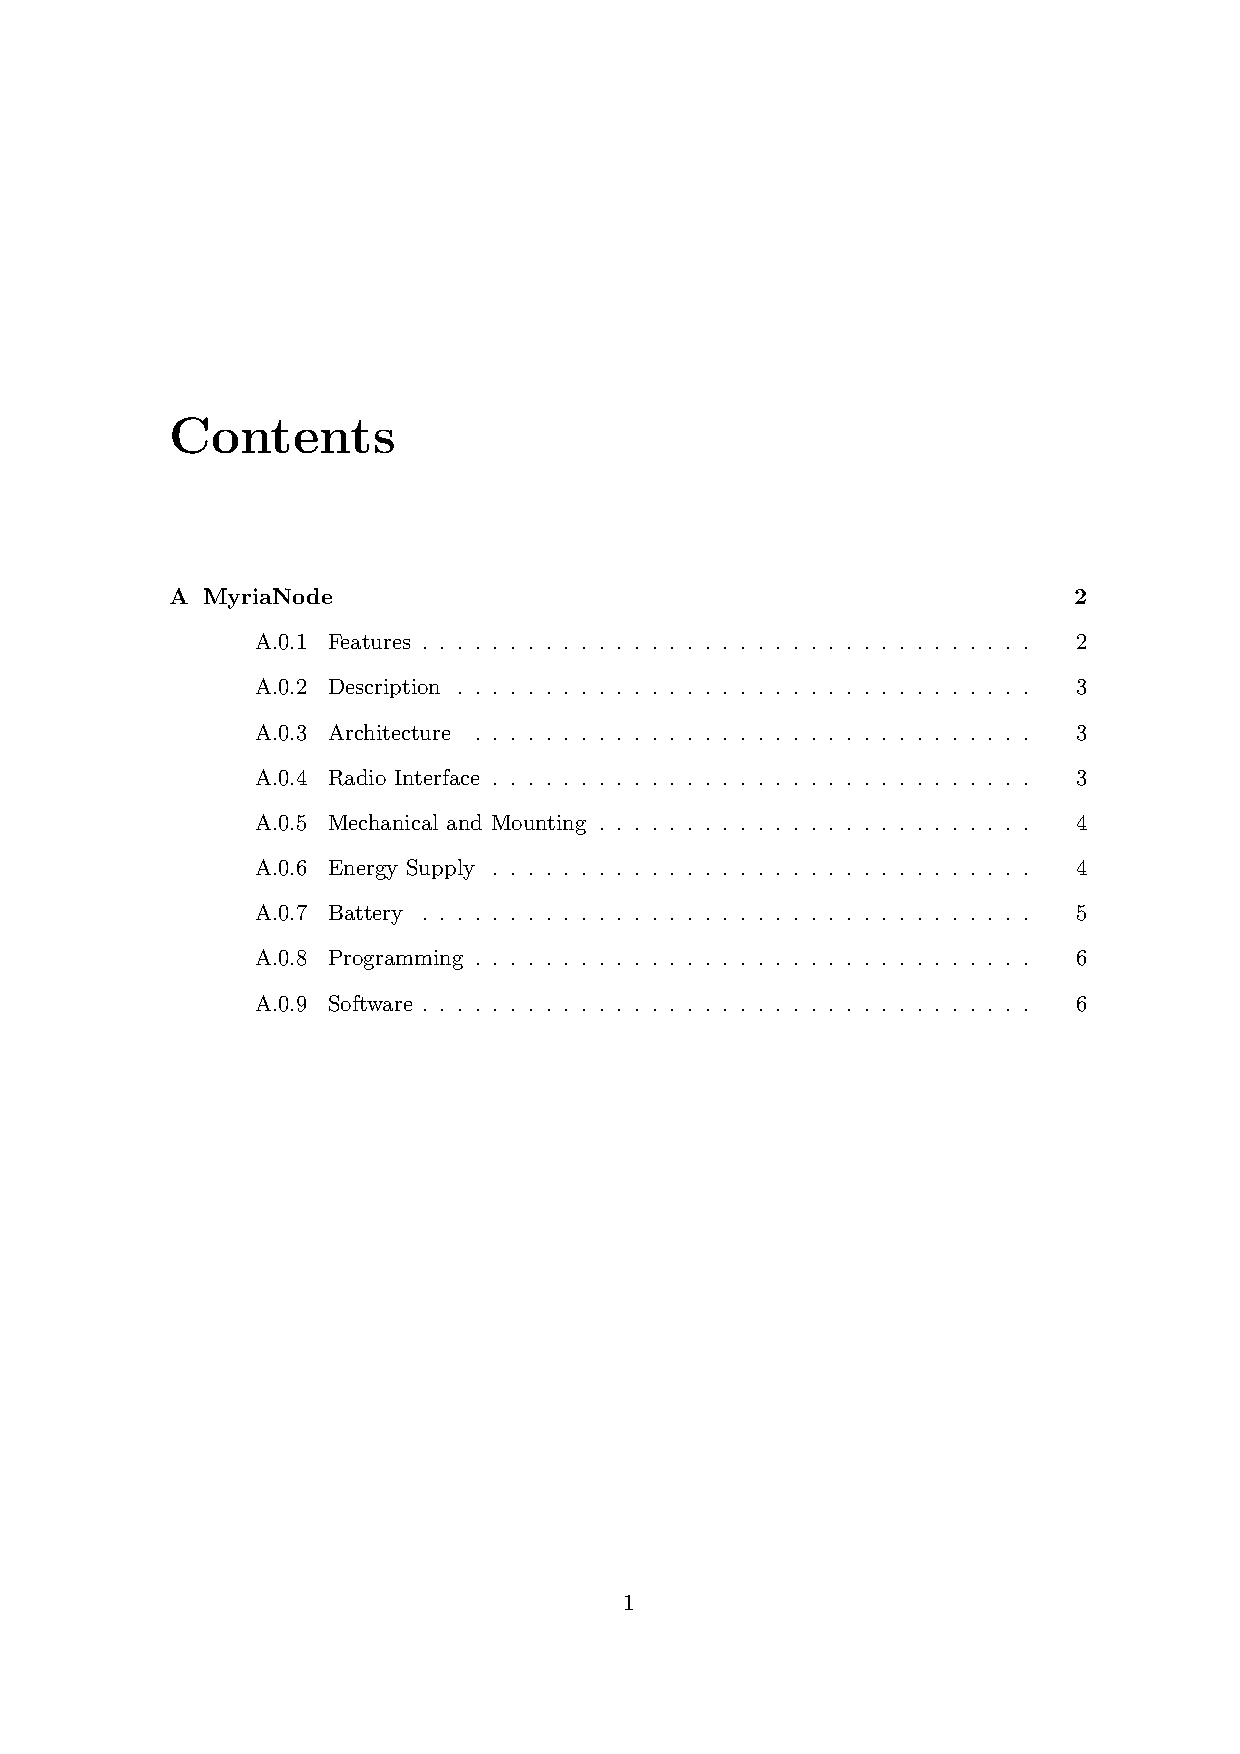
\includegraphics[width=0.5 \textwidth]{myrianode} \caption{MyriaNode v2.0} \label{myrianode} \end{figure}
\subsubsection{Features}
\begin{itemize}
 \item 2.4 GHz ISM band
 \item Nordic nRF24L01 Radio
 \item Integrated 1/4$\lambda$ PCB antenna
 \item ATMega645 processor
 \item 64kB FLASH
 \item 4kB SRAM
 \item 2kB EEPROM
 \item 32kHz Crystal clock
 \item Size: 20 X 40 mm
 \item Single supply voltage: 1.9V - 3.6V
\end{itemize}
\begin{wrapfigure}{r}{0.5\textwidth}
\vspace{-50pt}
  \begin{center}
    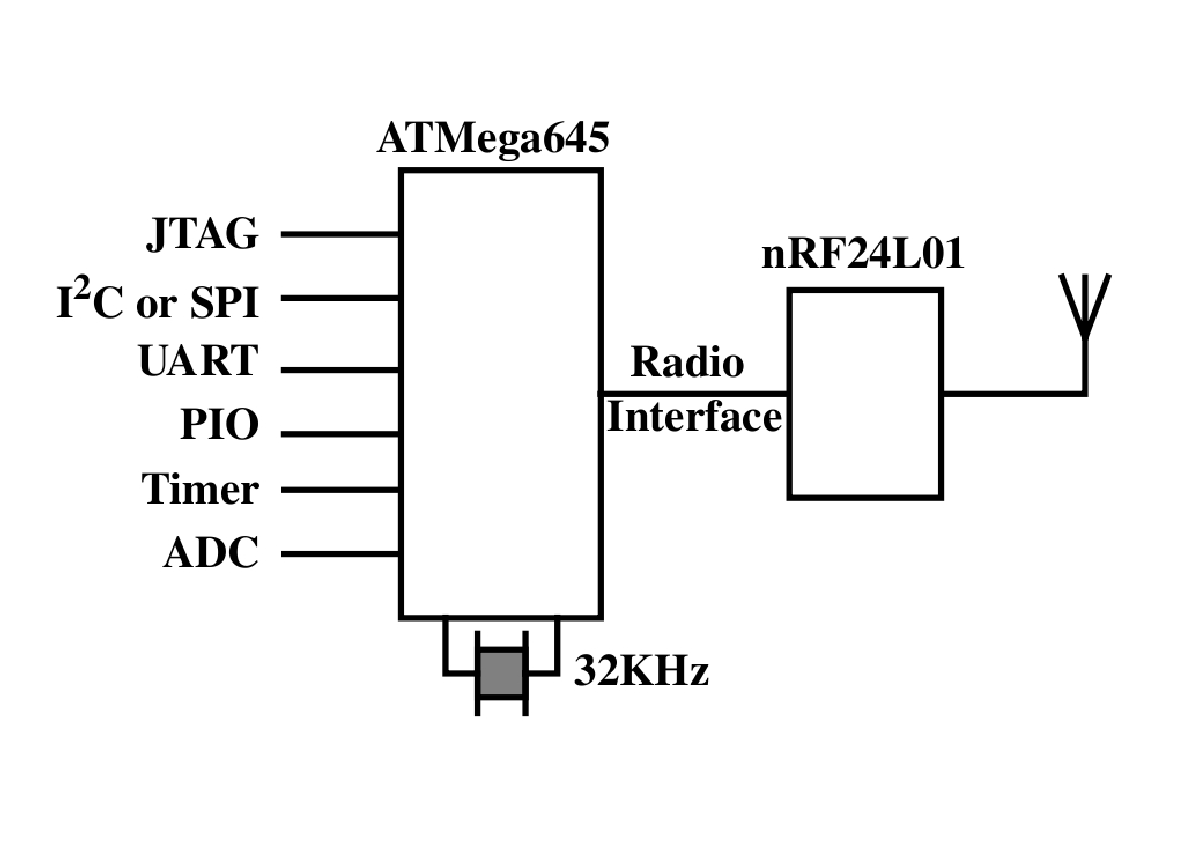
\includegraphics[width=0.48\textwidth]{myrianodearch}
  \end{center}
  \caption{MyriaNode architecture}
  \label{myrianodearch}
\end{wrapfigure}
\subsubsection{Description and architecture}
This Wireless Sensor Node is the second generation product for the MyriaNed project. It integrates a Nordic$\cite{nordic}$ radio module, antenna and embedded processor all on a PCB. The module is equipped with the software modules as they are being developed by one or more of the working groups of MyriaNed.
\subsubsection{Radio interface}
\begin{wrapfigure}{r}{0.5\textwidth}
\vspace{-30pt}
  \begin{center}
    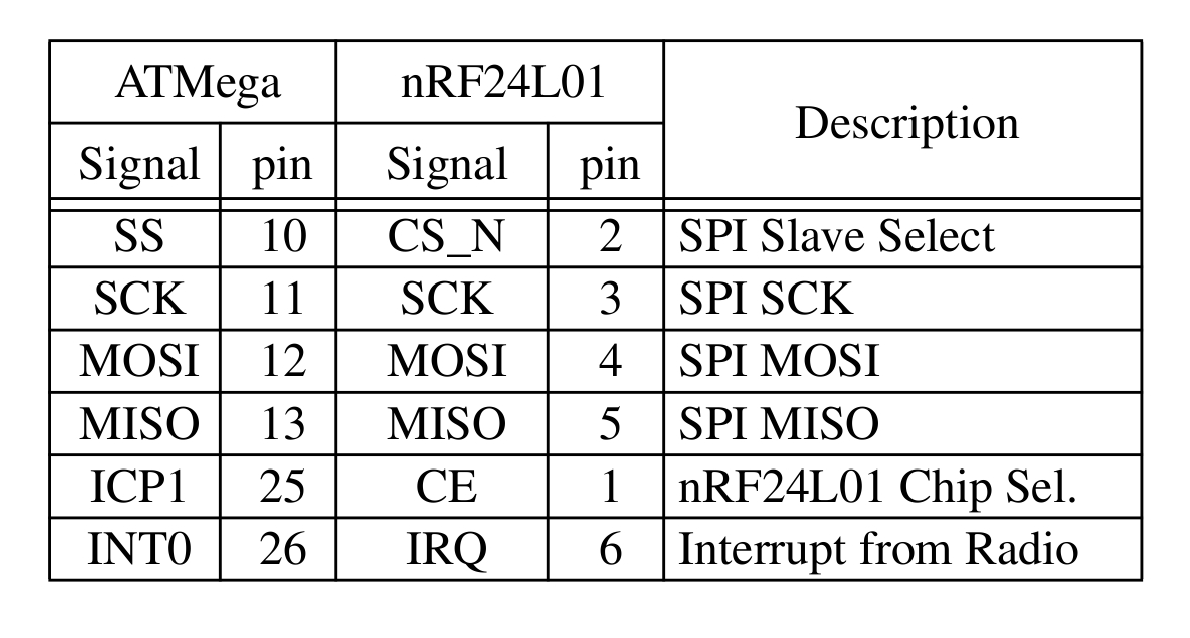
\includegraphics[width=0.48\textwidth]{table1}
  \end{center}
  \caption{Radio interfaces}
  \label{table1}
\end{wrapfigure}
SPI is used as interface between the processor and the radio, with the following interconnections:
%\begin{figure}[!h]
% \centering
%    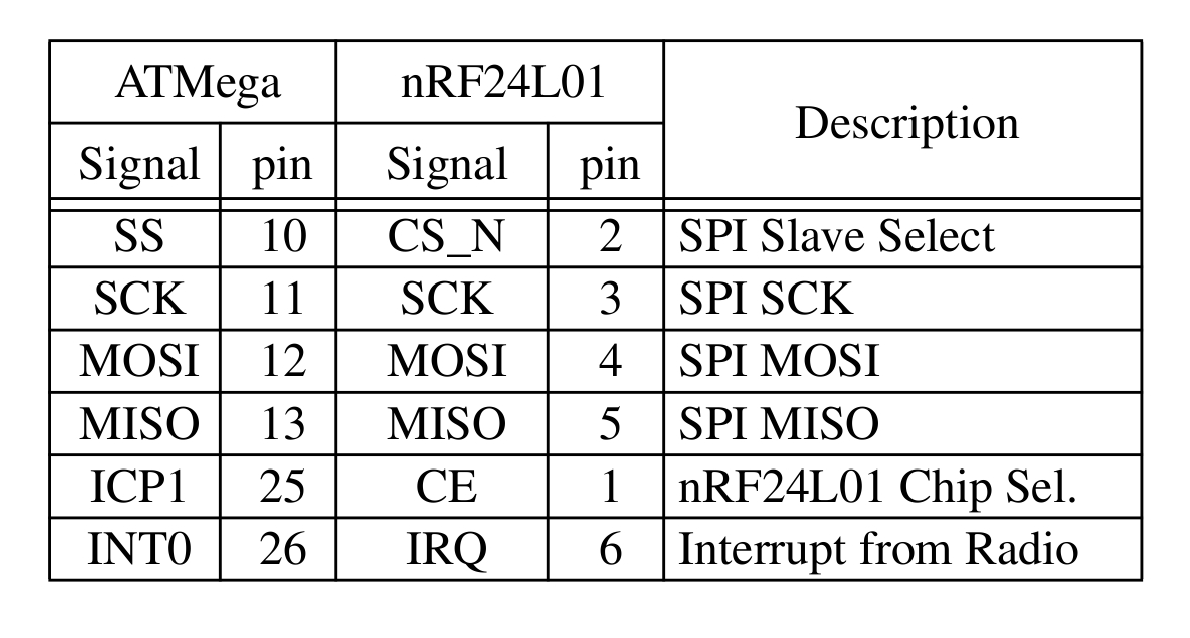
\includegraphics[width=0.6\textwidth]{table1}
%  \caption{Radio interfaces}
%  \label{table1}
%\end{figure}
\begin{figure}
 \centering
    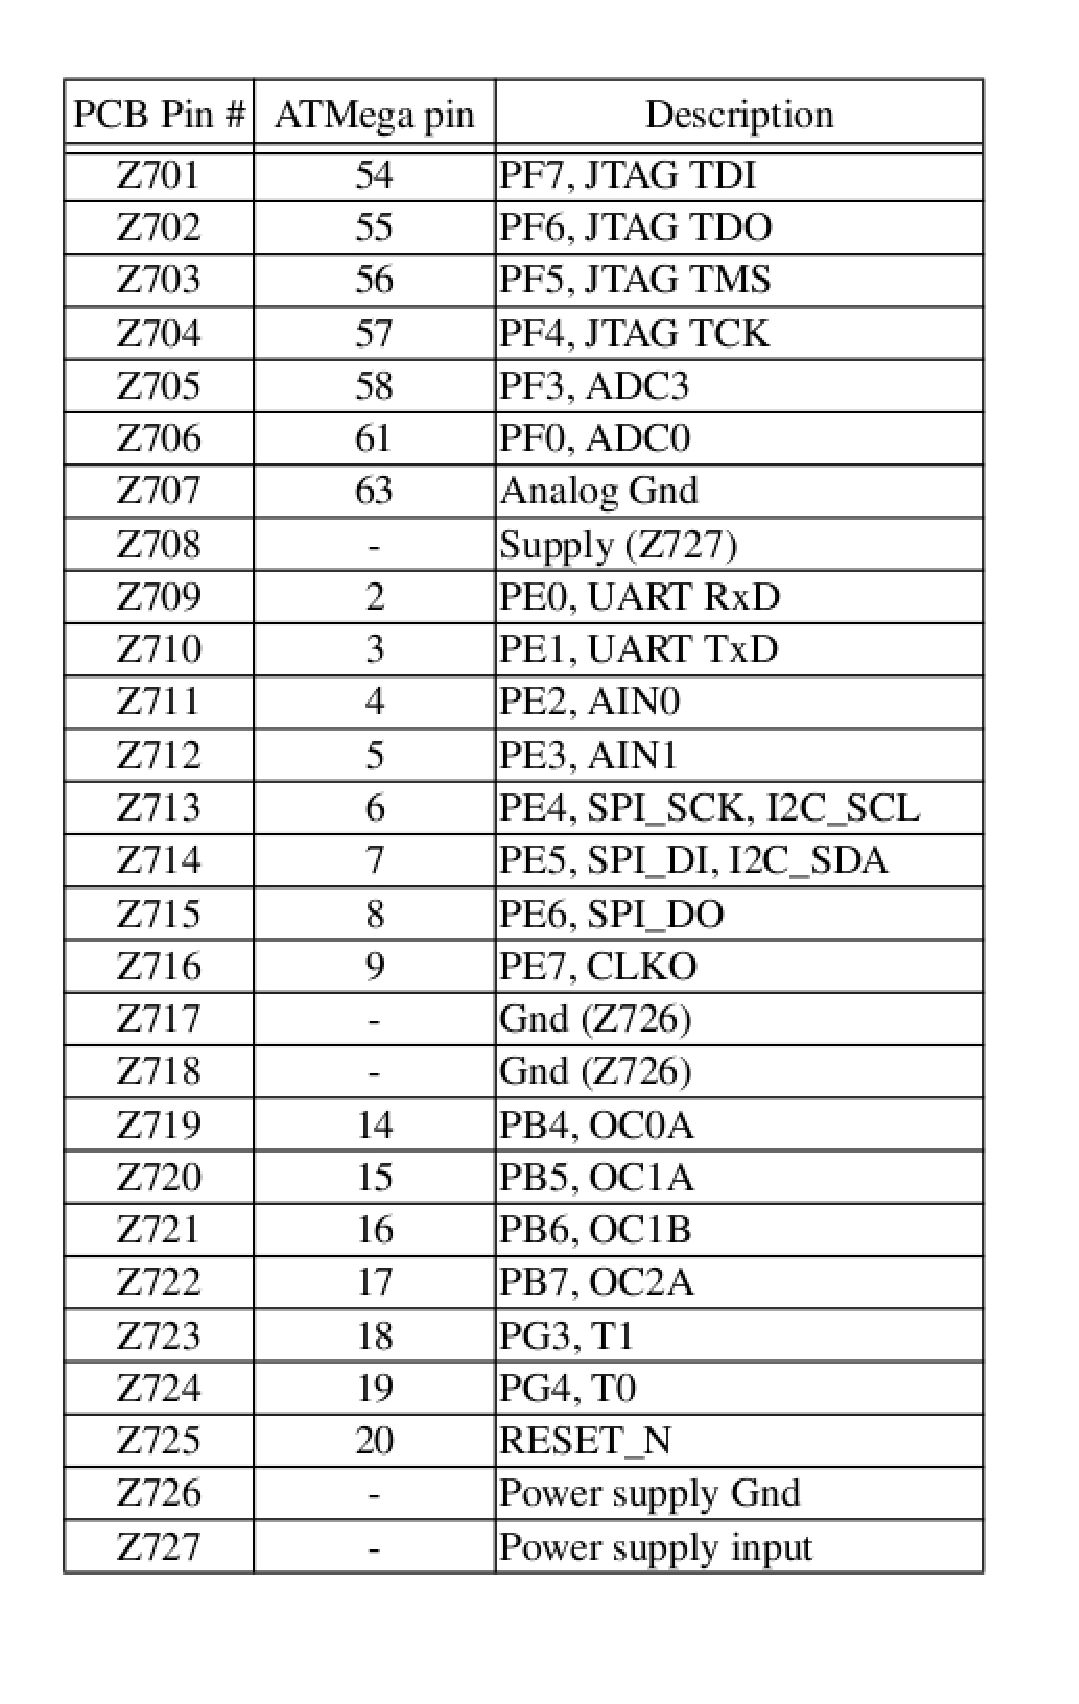
\includegraphics[width=0.6\textwidth]{table2}
  \caption{External interfaces}
  \label{table2}
\end{figure}
\subsubsection{Mechanical and Mounting}
\begin{wrapfigure}{r}{0.5\textwidth}
  \begin{center}
    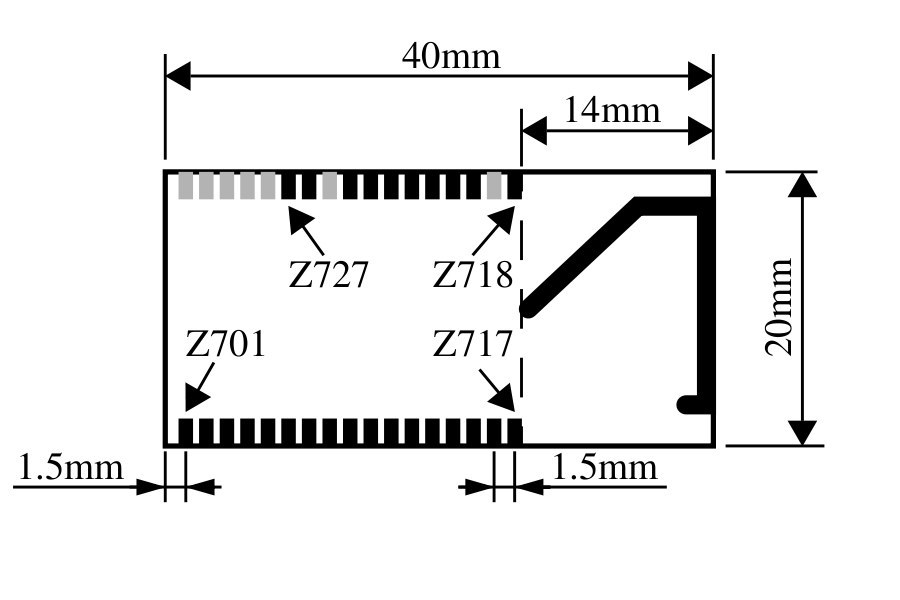
\includegraphics[width=0.48\textwidth]{myrianodephy}
  \end{center}
  \caption{MyriaNode dimentions}
  \label{myrianodephy}
\end{wrapfigure}
Figure $\ref{myrianodephy}$ shows the top (component) view of the module. It can be mounted as a Surface Mount Device (SMD) directly onto a base PCB. %The antenna area must be positioned% in free air.
\subsubsection{Energy Supply}
Both the embedded processor and the radio are connected to the same supply rail. The supply voltage must therefore remain in a range that meet the supply voltage specifications of both devices, which is: 1.9V - 3.6V. \paragraph*{}
In order to reduce conversion noise of the ADC to a minimum, the power decoupling circuit is implemented following the guidelines in the datasheet of the ATMega645$\cite{atmega}$. \paragraph*{}
\begin{wrapfigure}{r}{0.5\textwidth}
  \begin{center}
    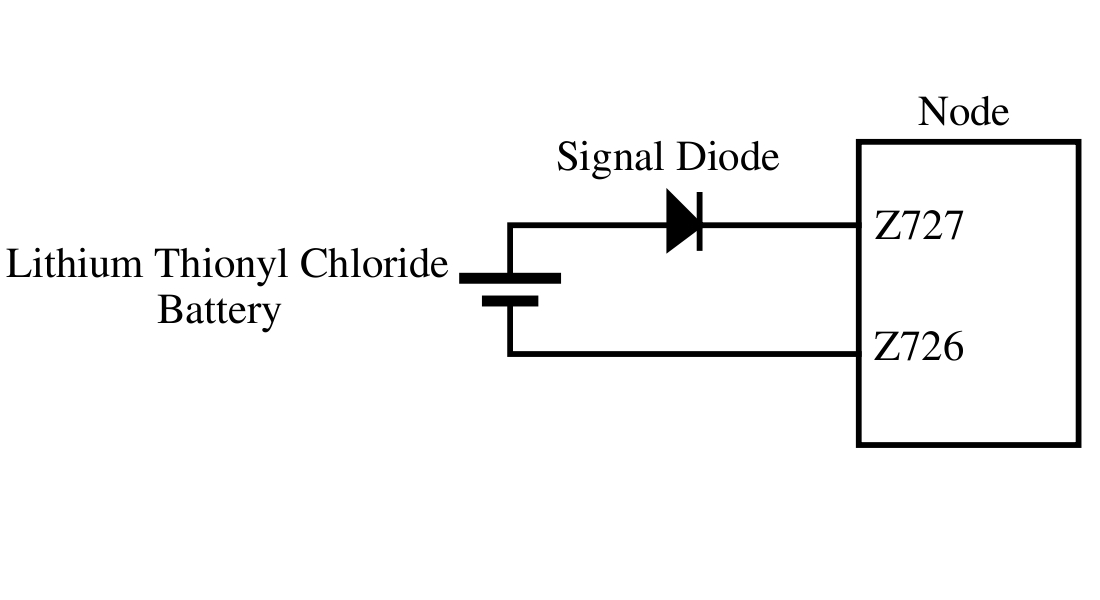
\includegraphics[width=0.48\textwidth]{battery}
  \end{center}
  \caption{Battery structure of  a MyriaNode}
  \label{battery}
\end{wrapfigure}
The energy consumption very much depends on the network parameters and application software. Under average conditions of a network cycle time of 1s, and a frame size of 32 bytes, the node can last for at least 5 years on a Lithium Thionyl Chloride battery of 900mAh.
%\paragraph*{}
%The voltage level of a new Lithium Thionyl Chloride battery is 3.67V, while the absolute maximum operating voltage of the nRF24L01 is 3.60V. This requires a voltage reduction circuit. The most simple one is to connect the node via a diode to the battery, as is shown in Figure $\ref{battery}$.
\subsubsection{Battery}
The ER14250$\cite{bat}$ from EMB is a Lithium Thionyl Chloride battery. It has a form factor of 1/2 AA size, and has a capacity of 1000mAh.
\subsubsection{Programming}
The node can be programmed and debugged via the JTAG interface. Although there are many second source suppliers of JTAG development tools, it is advised to use the AVR JTAGICE mkII from Atmel, ordering code: ATJTAGICE2$\cite{jtag}$.
\subsubsection{Software}
The software is documented by the other working groups of MyriaNed.
\addcontentsline{toc}{chapter}{References}
\begin{thebibliography}{\textbf{References}}
\bibitem{4}A.Tyrrell, and et al. "Firefly synchronization in ad hoc networks," in Proc. MiNEMA Workshop, February, 2006.
\bibitem{correlation}A.Ebner and et al. "Decentralized Slot Synchronization in Highly Dynamic Ad Hoc Networks," Wireless Personal Multimedia Communications, vol.2, pp. 494- 498, 2002.
\bibitem{11}C.Cordeiro and D.Agrawal. "Wireless sensor networks", Ad hoc and Sensor Networks Theory and applications. p.429-441. World Scientific Publishing. 2006.
\bibitem{gossip}D.Gavidia, S.Voulgaris, and M. van Steen. "A gossip-based distributed news service for wireless mesh networks,". In Proceedings 3rd IEEE Conference on Wireless On demand Network Systems and Services (WONS), Les Menuires, France, January 2006.
\bibitem{taxonomy}E.Anceaume and I.Puaut."A taxonomy of clock synchronization algorithms," IRISA Research Report No. PI1103, IRISA, 1997.
\bibitem{mutualsync}E.Souour and M.Nakagawa."Mutual decentralized synchronization for intervechicle communications," IEEE Transactions and Vehicular Technology, Vol.48, Issue 6, pp.2015-2027, 1999.
\bibitem{1}F.Zhao and  L.Guibas. "Time synchronization", Wireless Sensor Networks: an Information Processing approach. pp.107-108. Elsevier. 2004.
\bibitem{16}G.Werner-Allen and et al. "Firefly-inspired sensor network synchronicity with realistic radio effects," Proceedings of the 3rd international conference on Embedded networked sensor systems, San Diego, California. November 2005.
\bibitem{10}H.Karl and A.Willig. "Introduction" in Protocols and Architectures for Wireless Sensor Networks. pp. 3-6. Wiley. July 2006.
\bibitem{19}Dallas semiconductor."Crystal considerations with Dallas Real time clocks," Available online http:\slash \slash pdfserv.maxim-ic.com\slash en\slash an\slash AN58.pdf [Accessed on July 15,2008].
\bibitem{18}Golledge frequency products."SW Watch crystal temp mil," Available online http:\slash \slash www.golledge.co.uk\slash pdf\slash products\slash xtl$\_$sm\slash cc7v.pdf [Accessed on July 15,2008].
%\bibitem{omnet}$http://www.omnetpp.org$.
\bibitem{kalm}G.Welch and G.Bishop. "The kalman filter," University of North Carolina. Avalable online http:\slash \slash www.cs.unc.edu\slash ~welch\slash kalman\slash  [Accessed on June 10, 2008].
%\bibitem{chess}$http://www.chess.nl$.
\bibitem{myrianed}MyrianNed project. "Project description," Available online. http:\slash \slash www.chess.nl\slash en\slash home\slash Innovatie\slash Onderzoek\slash MyriaNed [Accessed on August 3, 2008].
\bibitem{nordic}Nordic semiconductor. Datasheet.Available online http:\slash \slash www.nordicsemi.no\slash files\slash Product\slash data$\_$sheet\slash Product$\_$Specification$\_$nRF24L01$\_$1.0.pdf [Accessed August 3, 2008].
\bibitem{jtag}Atmel. "AVR JTAGICE mkII," Available online. http:\slash \slash www.atmel.com\slash dyn\slash resources\slash prod$\_$documents\slash doc2489.pdf [Accessed August 3, 2008].
\bibitem{atmega}Atmel "8-bit Microcontroller with In-System Programmable Flash," Available online. http:\slash \slash www.atmel.com\slash dyn\slash resources\slash prod$\_$documents\slash doc2570.pdf. [Accessed August 3, 2008].
\bibitem{bat}Nrgeurope. Battery datasheet. Available online. http:\slash \slash www.nrgeurope.com [Accessed August 3, 2008].
\bibitem{2}J.Elson, L.Girod and D.Estrin. "Fine-grained network time synchronization using reference broadcasts," Proceedings of the 5th Symposium on Operating Systems Design and Implementation, Boston, USA, 2002.
\bibitem{7}J.Elson and D.Estrin. "Time Synchronization for Wireless Sensor Networks," In Proceedings of the 15th International Parallel and Distributed Processing Symposium. IEEE Computer Society, April 23-27. 2001.
\bibitem{9}K.Romer. "Time Synchronization in Ad Hoc Networks," In Proceedings of the Second ACM International Symposium on Mobile Ad Hoc Networking and Computing, Long Beach, California. 2001.
\bibitem{gradient2}L.Meier,and L.Thiele. "Gradient clock synchronization in sensor networks," Technical report, Computer Engineering and Networks Laboratory. Swiss Federal Institute of Technology Zurich, 2005.
\bibitem{5}"NTP Public Services Project," Available online http:\slash \slash support.ntp.org\slash bin\slash view\slash Main\slash WebHome [Accessed on June 12,2008].
%\bibitem{devlab}Project description. Available online http://www.devlab.nl [Accessed on August 6, 2008].
\bibitem{chess}Company profile. Available online http://www.chess.nl [Accessed on August 6, 2008].
\bibitem{3}Q.Yang, and et al. "A Decentralized Slot Synchronization Algorithm for TDMA-Based Ad Hoc Networks," Wireless Communications, Networking and Mobile Computing, Vol., Issue,21-25, pp. 1717 - 1721, 2007.
\bibitem{17}Q.Yang and J.Shi. "An interference elimination method for decentralized slot synchronization in TDMA-based wireless ad hoc network," Intelligent Signal Processing and Communication Systems, pp.236-239, 2007.
\bibitem{pieter}P.Anemaet. "Determining G-MAC potential with $\{$S,L,SCP$\}$-MAC," Masters thesis. Technische Universteit Delft. Delft. August 2008.
\bibitem{median}R.Tjoa and et al. "Clock drift reduction for relative time slot tdma-based sensor networks," Personal, Indoor and Mobile Radio Communications, Vol.2, 5-8 , pp.1042 - 1047. Sept. 2004.
\bibitem{6}R.John. "Introduction to Quartz Frequency Standards," Technical Report SLCET-TR-92-1, Army Research Laboratory, Electronics and Power Sources Directorate. October 1992.
\bibitem{gradient}R. Fan and N. Lynch. "Gradient clock synchronization," In Proceedings of the twenty-third annual ACM symposium on Principles of distributed computing, pp.320-327. ACM Press, 2004.
\bibitem{clockwhite}Symmetricom, Inc. "Stochastic Model Estimation of network time variance," Available online http:\slash \slash www.symmttm.com\slash pdf\slash Network$\_$Timing\slash wp$\_$Stochastic$\_$Model.pdf [Accessed August 3,2008].
\bibitem{texas}S.Raje and Q.Liang. "Time synchronization in Network-centric sensor networks," Radio and Wireless Symposium IEEE, pp.333-336. 2007.
\bibitem{14}S.PalChaudhuri and et al. "Adaptive Clock Synchronization in Sensor Networks," Information Processing in Sensor Networks, pp.340- 348, 2004.
\end{thebibliography}
\end{document}
